%
%

%
%

%
\documentclass[robotics,article,accept,pdftex,oneauthor]{Definitions/mdpi} 
%
%

%
%

%
%

%
%
%
%
%
%
%
%

%
%
%
%
%
%

%
%
%
%

%
%
%
%

%
%
%
%

%
%
\firstpage{1} 
\makeatletter 
\setcounter{page}{\@firstpage} 
\makeatother
\pubvolume{1}
\issuenum{1}
\articlenumber{0}
\pubyear{2025}
\copyrightyear{2025}
\externaleditor{ Swaminath Venkateswaran, Jong-Hyeon Park } %
\datereceived{18 January 2025} 
\daterevised{24 February 2025} %
\dateaccepted{25 February 2025} 
\datepublished{ } 
%
%
\hreflink{https://doi.org/} %
%
%
%
%

%
%
%


%
%
%
\usepackage{overpic}
\usepackage{wrapfig}
\usepackage{pgfplots} %
\usepackage{bm}
%
\usepackage{makecell} %
\usepackage[per-mode=symbol]{siunitx} %
\renewcommand{\hl}[1]{#1}

%
\newif\ifgrammarly
%

\ifgrammarly
  \usepackage[none]{hyphenat} %
  \usepackage[nomarkers,notables]{endfloat} %
  \usepackage{endnotes} %
  \renewcommand{\footnote}{\endnote}
\fi


%
%
%

%
%
\Title{Dimensional Synthesis of Parallel Robots Using Bilevel Optimization for Design Optimization and Resolution of Functional Redundancy}

%
\TitleCitation{Dimensional Synthesis of Parallel Robots Using Bilevel Optimization for Design Optimization and Redundancy Resolution}

%
\newcommand{\orcidauthorA}{0000-0001-7952-7363} %
%

%
\Author{Moritz Schappler
\orcidA{}}

%

%
\AuthorNames{Moritz Schappler}

%
%
%
%

%
%
%

%
%
\isAPAStyle{%
       \AuthorCitation{Schappler, M.}
         }{%
        \isChicagoStyle{%
        \AuthorCitation{Moritz Schappler.}
        }{
        \AuthorCitation{Schappler, M.}
        }
}

%
\address[1]{%
Institute of Mechatronic Systems, Leibniz University Hannover, 30823 Garbsen, Germany;  moritz.schappler@imes.uni-hannover.de}

%
%

%
%
%
%

%

%

%
\abstract{%
%
Parallel-kinematic machines or parallel robots have only been established in a few applications where their advantage over serial kinematics due to their high payload capacity, stiffness, or dynamics with their limited workspace-to-installation-space ratio pays out.
However, some applications still have not yet been sufficiently or satisfactorily automated in which parallel robots could be advantageous.
%
As their performance is much more dependent on their complex dimensioning, an automated design tool---not existing yet---is required to optimize the parameterization of parallel robots for applications. Combined structural and dimensional synthesis considers all principally possible kinematic structures and performs a separate dimensioning for each to obtain the best task-specific structure. However, this makes the method computationally demanding.
The proposed computationally efficient approach for dimensional synthesis extends multi-objective particle swarm optimization with hierarchical constraints.
A cascaded (bilevel) optimization includes the design optimization of components and the redundancy resolution for tasks with rotational symmetry, like milling.
%
Two case studies for different end-effector degrees of freedom demonstrate the broad applicability of the combined structural and dimensional synthesis for symmetric parallel robots with rigid links and serial-kinematic leg chains.
%
The framework produces many possible task-optimal structures despite numerous constraints and can be applied to other problems \hl{as an open-source} \textsc{Matlab} toolbox. %
%
%
}

%
\keyword{parallel robot; parallel-kinematic machine; dimensional synthesis; bilevel optimization; constraint handling; design optimization; redundancy resolution} %


%
%
%
%

%
%
%

%
%
%
%

%
%
%
%

%
%
%

%
%
%

%
%
%
%

%
%
%
%
%
%
%
%
%
%
%
%

\renewcommand{\vec}[1]{\boldsymbol{#1}}
\newcommand{\dvec}[1]{\dot{\boldsymbol{#1}}}
\newcommand{\ddvec}[1]{\ddot{\boldsymbol{#1}}}
\newcommand{\transp}{\mathrm{T}}
\newcommand{\transpose}{\transp}	
\newcommand{\ind}[1]{\mathrm{#1}}	%
\newcommand{\propername}[1]{#1} %
\DeclareMathOperator*{\argmin}{argmin}
\newcommand{\point}[1]{\mathrm{#1}}
\newcommand{\indks}[1]{\mathrm{#1}} %
\newcommand{\ks}[1]{(\ind{CS})_{#1}} %
\newcommand{\rovec}[2]{{_{(#1)}\vec{r}_{{#2}}}}
\newcommand{\rotmat}[2]{{^{#1\!}\vec{R}}_{#2}}
\newcommand{\ortvek}[4]{{ }_{(#1)}{\boldsymbol{#2}}^{#3}_{#4} }

\newcommand{\vecRes}[0]{\vec{\delta}} %
\newcommand{\vecResR}[0]{\vec{\psi}} %

%
\newcommand{\refl}[1]{\hypersetup{linkcolor=black}\ref{#1}\hypersetup{linkcolor=[RGB]{0 128 128}}} %
\newcommand{\hyperrefl}[2]{\hypersetup{linkcolor=black}\hyperref[#1]{#2}\hypersetup{linkcolor=[RGB]{0 128 128}}} %

% File created by structsynth_robot_table.m. Do not change manually!
\newcommand{\PKMTTTnumkinematics}{38}
\newcommand{\PKMTTTnumkinematicswithvalidact}{28}
\newcommand{\PKMTTTnumactuation}{118}
\newcommand{\PKMTTTnumvalid}{92}
\newcommand{\PKMTTTnuminvalid}{26}

% File created by structsynth_robot_table.m. Do not change manually!
\newcommand{\PKMTTTRnumkinematics}{30}
\newcommand{\PKMTTTRnumkinematicswithvalidact}{18}
\newcommand{\PKMTTTRnumactuation}{102}
\newcommand{\PKMTTTRnumvalid}{61}
\newcommand{\PKMTTTRnuminvalid}{41}

% File created by structsynth_robot_table.m. Do not change manually!
\newcommand{\PKMTTTRRnumkinematics}{16}
\newcommand{\PKMTTTRRnumkinematicswithvalidact}{10}
\newcommand{\PKMTTTRRnumactuation}{35}
\newcommand{\PKMTTTRRnumvalid}{21}
\newcommand{\PKMTTTRRnuminvalid}{14}

% File created by structsynth_robot_table.m. Do not change manually!
\newcommand{\PKMTTTRRRnumkinematics}{47}
\newcommand{\PKMTTTRRRnumkinematicswithvalidact}{47}
\newcommand{\PKMTTTRRRnumactuation}{234}
\newcommand{\PKMTTTRRRnumvalid}{223}
\newcommand{\PKMTTTRRRnuminvalid}{11}




%
\begin{document}

%

\section{Introduction}

%
%
%

Despite a research history of more than three decades and potential theoretical advantages~\cite{Merlet2006}, \emph{parallel robots} %
have not been successful in the market yet except for single examples~\cite{RussoZhaLiuXie2024}.
Parallel robots can, in principle, encounter some disadvantages of serial robots, especially regarding dynamics, accuracy, moving mass, and related energy consumption.
Since many problems
%
of fundamental research have already been solved \cite{BriotBur2023,ShaoZhaCar2023,RussoZhaLiuXie2024}, the still high and increasing publication activity on rigid parallel robots can be attributed to reaching broader (yet non-commercial) applications. \emph{Further research on their optimal design is required}, as optimal and task-specific design is essential for the deployment of parallel robots to provide new and improved automation of tasks.
%
%
This paper \emph{contributes} to that field by \emph{combining methods} for structural and dimensional synthesis (Section~\ref{sec:previouswork_parrob}), resolution of functional redundancy (Section~\ref{sec:previouswork_taskred}), and design optimization (Section~\ref{sec:previouswork_desopt}) in one \emph{framework} based on the concept of \emph{bilevel optimization}. There, two optimization problems are nested into each other, which holds for engineering design problems \cite{SinhaMalDeb2017}, such as robot synthesis.

\subsection{Structural and Dimensional Synthesis of Parallel Robots}
\label{sec:previouswork_parrob}

%
%
%
%
%

The systematic \emph{structural synthesis} of parallel robots (for finding the number and alignments of joints and kinematic chains called legs) was driven by mathematical formulations such as screw theory \cite{KongGos2007}, the theory of linear transformations \cite{Gogu2008}, and other concepts to take into account the higher complexity of parallel over serial robots.
The importance of the \emph{dimensional synthesis} (for determining numerical values for the parameters) was highlighted by several authors, e.g., \cite{Frindt2001} (p. 124), \cite{Krefft2006} (p. 175), and \cite{Merlet2006} (p. 25), as being at least as important for the robot performance as the structural synthesis. This distinguishes parallel from serial robots, where the dimensioning is much more intuitive. Specific further studies on dimensional synthesis have been performed for single parallel robots, e.g., \cite{Kirchner2000,StockMil2003,RaoRaoSah2005,Krefft2006,CarboneOttCec2007,KelaiaiaComZaa2012,Miller2004,LaribiRomZeg2007,LiuHuaMeiZha2012,Daake2012,JamwalHusXie2015}.
Many more references could extend the non-exhaustive list since proper dimensioning is necessary for all \hl{parallel-robot prototypes}. %
The concept of \emph{combined structural and dimensional synthesis} optimizes multiple structures simultaneously and only then selects the best structure. 
This was first realized by \cite{Krefft2006,Kirchner2000} in a basic example of a few non-redundant parallel robots. The concept was only pursued systematically by a few others, such as \cite{Prause2016} for three-DoF parallel robots, \emph{leaving aspects like functional redundancy uncovered}.

%


%

\subsection{Functional Redundancy}
\label{sec:previouswork_taskred}
%

%
%
The operational space is the physical motion space of the robot end effector, and the task space is the sub-set coordinate space to define a robot task. 
These spaces are congruent for most but not all tasks \cite{SciaviccoSicVilOri2009} (p. 88).
Many \emph{industrially relevant tasks} %
like welding, milling, or drilling only require five degrees of freedom (DoF) in their task space, while one coordinate of the six-DoF operational space can be set arbitrarily, resulting in \emph{functional redundancy}.
%
The aspect was mainly investigated for serial robots. %
For parallel robots, kinematic models are more complex and the minimal coordinates are already the operational-space coordinates; therefore, fewer publications use dedicated models \cite{SchapplerTapOrt2019c} but rather incorporate the aspect into existing models by gradient-descent \cite{AgarwalNasBan2016} or within an overlying optimization \cite{MerletPerDan2000,OenWan2007,CorinaldiAngCal2016,SantosSil2017,GaoCheGaoXia2019,Schappler2023_ICINCOLNEE}, which can become computationally expensive.

Functional redundancy has not yet been considered explicitly \emph{as part of the dimensional synthesis} of parallel robots.
In the structural synthesis, no dedicated consideration is necessary since the operational space has to be regarded there. 
Tasks or manipulators with five degrees of freedom are missing in the relevant works on \emph{combined synthesis}, e.g., in \cite{Krefft2006,Prause2016,Ramirez2018}. 
%
%
Functional (or task) redundancy may look counter-intuitive for task-specific robots at first.
Including this in the synthesis is motivated by many parallel robots having six end-effector degrees of freedom. 
In contrast, five DoFs are difficult to realize. %
Excluding functionally redundant robots from the synthesis \emph{would strongly limit the combined-synthesis approach for these most relevant tasks.}
As shown in the literature, \emph{exploiting functional redundancy is critical for the performance and feasibility of robots in these tasks.}

%
%
%
%
%
%
%
%
%
%

\subsection{Design Optimization}
\label{sec:previouswork_desopt}
%

%
Lifting the structural assumptions from the literature requires a more detailed look at those non-kinematic parameters of parallel robots subject to \emph{design optimization}.
Higher internal bending moments of multi-joint leg chains may require stronger dimensioning of limbs, which increases self-collisions. 
Required high actuator torques may lead to bulky motors that can not be integrated into the construction anymore. 
Static compensation springs may reduce the latter effect if they are well designed, eventually favored by a specific kinematic structure.
Including these aspects is \emph{necessary for a robust comparison of one kinematic structure to another} and is investigated together with the other facets.

%
\subsection{Motivation and Structure of the Paper}
\label{sec:previouswork_summmary}
%

%
  %
%
%

Methods for the \emph{combined structural and dimensional synthesis} of serial and parallel robots have been proposed and provide \emph{well-argued advantages over a classical two-stage synthesis.}
Furthermore, many methods exist for the resolution of functional redundancy.
%
%
%
However, the two concepts have yet to be combined even though \emph{tasks enabling functional redundancy are the most industrially relevant type of task.}
Moreover, design optimization is mainly covered for serial rather than parallel robots.
%
%
%
%
%
%
%
%
%
%
By missing tools for systematic optimization, the performance of parallel robots cannot be fully exploited, and \emph{industrial tasks may be realized in a sub-optimal way or not at all if no robot exists for them yet.}

%
The overall workflow of the combined robot synthesis is summarized in Figure~\ref{fig:comb_struct_dim_synth}. %
%
Next; the single aspects are elaborated in more detail in comparison to existing works in Section~\ref{sec:relatedwork}.
The materials and methods to encounter the gaps in the literature are the subject of Section~\ref{sec:materials}, followed by results in the form of two case studies in Sections~\ref{sec:eval_water} and~\ref{sec:eval_handlingfreerotation} and a discussion and conclusions in Sections~\ref{sec:discussion} and~\ref{sec:conclusions}.

%
%

%
%
%


%


%
%
%
%
%
%
%
%


\begin{figure}[H]
\begin{adjustwidth}{-\extralength}{0cm}
  \centering
  \graphicspath{{./Figures/}}
  \input{./Figures/comb_struct_dim_synth.pdf_tex}
\end{adjustwidth}
\caption{\hl{Overview} %
  %
  %
  %
  of the procedure for combined structural and dimensional synthesis, which structures the paper. Abbreviations: \hl{degree of freedom (DoF)}; optimal (opt.)} %
\label{fig:comb_struct_dim_synth}
\end{figure} 



\section{Related Work}

%
%
%
\label{sec:relatedwork}

%
%


The literature relevant to the dimensional robot synthesis is discussed in the following subsections.
First, preliminaries regarding the kinematics modeling of parallel robots are introduced in Section~\ref{sec:ds_parrob_preliminaries}.
The proposed framework of hierarchical optimization from Section~\ref{sec:materials} structures the remaining text.
%
%
It is separated into an overview of approaches for the robot-synthesis problem in general in Sections~\ref{sec:ds_soa_design}--%
\ref{sec:ds_combstructgeomsynth}, followed by the optimization of kinematic parameters (Section~\ref{sec:ds_soa_kinpar}), other design parameters (Section~\ref{sec:ds_soa_despar}), and robot motion (Section~\ref{sec:ds_soa_motionplanning}).
%
Optimization methods are discussed in Section~\ref{sec:ds_soa_optim} regarding their usability within the different optimization problems of the robot synthesis.
%
%
%
%
%

\subsection{Preliminaries on Parallel Robots: Functional Redundancy and Kinematic Constraints}
\label{sec:ds_parrob_preliminaries}



%

%

For a robot manipulator, \emph{intrinsic redundancy} exists if the joint space has a higher dimension than the operational space. %
\emph{Functional redundancy} is defined as an operational-space dimension higher than the task-space and the joint-space dimension \cite{ConkurBuc1997,SciaviccoSicVilOri2009,HuoBar2008,LegerAng2016}. %
%
%
Both forms of redundancy are combined under the term ``kinematic redundancy'' \cite{SciaviccoSicVilOri2009} (p. 88).
%



The occurrence of functional redundancy is illustrated in Table~\ref{tab:task_vs_robot_dof}, where the most relevant spatial robot operational-space degrees of freedom (in rows; ``robot DoF'') and task-space DoFs (in columns; ``task DoF'') are combined in a matrix, and the cells show the effect on the degree of functional redundancy $n_\mathrm{R}$. %
In some tasks, $n_\mathrm{C}$ additional constraints have to be defined, which implicitly corresponds to the definition of coordinates.


\begin{table}[H]
  \newcommand{\no}{{\color{red}$\boldsymbol\times$}}
  \caption[Overview of combinations of robot end-effector DoFs and task DoFs]{\hl{Overview} %
  %
   %
   %
    of combinations of robot end-effector DoFs (rows) and task DoFs (columns) with the degree of redundancy $n_\mathrm{R}$ \hl{(highlighted in blue)} and number of resulting constraints $n_\mathrm{C}$. If not given, $n_\mathrm{R}~{=}~0$ or $n_\mathrm{C}~{=}~0$ holds. Naming of tasks f.l.t.r.: rotation fixed (3T0R); {only} planar rotation {that is} arbitrary (3T0*R); only planar rotation {that is} defined (3T1R), pointing (3T2R); free motion in space (3T3R). The symbol ``\no'' marks impossibility \hl{and row and column headings use bold font}.}
  \label{tab:task_vs_robot_dof}
  %
    \begin{tabularx}{\textwidth}{lCcCCC} 
      \toprule
      \textbf{Task DoFs} $\rightarrow$ & \textbf{3T0R}  & \textbf{3T0*R} & \textbf{3T1R}  & \textbf{3T2R}  & \textbf{3T3R}  \\ 
      \midrule
      \textbf{Robot DoFs} \hl{$\downarrow$} %
      %
      & \textbf{(Rot. Fix.)}&\textbf{(Rot. Arbitr.)} & \textbf{(Rot. Def.)} & \textbf{(Pointing)} & \textbf{(Free)} \\
      \midrule
      \hl{\textbf{3T0R}} %
      %
      (3)  & $n_\mathrm{R}~{=}~0$ & $n_\mathrm{R}~{=}~0$ &  \no & \no & \no  \\
      \hl{\textbf{3T0*R}} (3)  & \no & $n_\mathrm{R}~{=}~0$ &  \no & \no & \no  \\
      \hl{\textbf{3T1R}} (4)  & $n_\mathrm{C}~{=}~1$ & \textcolor{blue}{$n_\mathrm{R}~{=}~1$} & $n_\mathrm{R}~{=}~0$ & \no & \no \\
      \hl{ \textbf{3T2R}} (5)  & $n_\mathrm{C}~{=}~2$ & $n_\mathrm{C}~{=}~2$ & $n_\mathrm{C}~{=}~1$  & $n_\mathrm{R}~{=}~0$ &  \no \\
      \hl{\textbf{3T3R}} (6)  & $n_\mathrm{C}~{=}~3$ & $n_\mathrm{C}{=}2$; \textcolor{blue}{$n_\mathrm{R}~{=}~1$} & $n_\mathrm{C}~{=}~2$  &  \textcolor{blue}{$n_\mathrm{R}~{=}~1$} & $n_\mathrm{R}~{=}~0$ \\
      \bottomrule
    \end{tabularx}
    %
\end{table}

Redundancy for \emph{parallel robots} has been extensively studied for the aspects of \emph{kinematic redundancy} (additional joints in a leg chain) or \emph{actuation redundancy} (additional actuators or actuated leg chains) \cite{LucesMilBen2017,GosselinSch2018}.
\emph{Functional redundancy} for parallel robots (more platform DoFs than required by the task) is distinguished since parallel robots are characterized by the platform DoFs as minimal coordinates, unlike serial robots, characterized by the joint DoFs.
Functional redundancy is addressed less in the literature and is not mentioned in the otherwise extensive review articles \cite{LucesMilBen2017,GosselinSch2018} on redundancy for parallel robots.
%
In the following, one degree of functional redundancy is assumed, corresponding to the tool rotation in machining tasks (3T2R). %
Some references show the possibility of improving the performance and avoiding limits by exploiting functional redundancy, such as for a planar 3-\underline{R}RR %
%
robot \cite{AlbaGomezWenPam2005,KotlarskiDoHeiOrt2010,AgarwalNasBan2016,GaoCheGaoXia2019}, for a 6-\underline{P}US \cite{OenWan2007} and 6-U\underline{P}S robot \cite{MerletPerDan2000,OenWan2007,Schappler2023_ICINCOLNEE}, and a combination of two~three-DoF parallel robots \cite{CorinaldiAngCal2016}.
The %
%
notation for parallel robots includes the number of identical leg chains and the type of their joints counted from the base: revolute (R),  prismatic (P), universal (U), and spherical (S). Underlining denotes an actuated joint.
In total, the possible improvement can be assumed to extend to all parallel robots since they are susceptible to singularities, joint limitations, and/or self-collisions. %
%


A general approach for a kinematics model of parallel robots is reported in introductory textbooks~\cite{Merlet2006,Gogu2008,BriotKha2015}. %
The considered parallel robot consists of $m$ legs with $n_i$ joint coordinates %
%
$\bm{q}_i$ each, connected at a moving platform.
Additionally to the active joints $\bm{q}_{\mathrm{a},i}$, explicitly all passive joints $\bm{q}_{\mathrm{p},i}$, including the platform-coupling joints, are part of the coordinates $\bm{q}_i$ of leg~$i$.
All $n_{\bm{q}}$ joint coordinates of the parallel robot are stacked in the vector $\bm{q}=[\bm{q}_1^\transp,\dots,\bm{q}_m^\transp]^\transp$, and all $n_{\bm{q}_\mathrm{a}}$ active joints are assembled in the vector $\bm{q}_\mathrm{a}=[q_{\mathrm{a},1},\dots,q_{\mathrm{a},m}]^\transp$. %

A sketch of the assembly of the robot's leg chains (corresponding to solving the inverse-kinematics problem) is depicted in Figure~\ref{fig:kinematic_constraints}a with the necessary coordinate systems for kinematic modeling adapted from \cite{BriotKha2015}, including a robot base frame $\ks{0}$, leg-chain base frames $\ks{\indks{A}_i}$, and cut coupling-joint frames $\ks{\indks{C}_i}$ at the end of the leg chains.
The desired pose of the moving-platform frame $\ks{\indks{D}}$ is expressed with the minimal coordinates $\bm{x}$. %

%

The relation between joint coordinates $\bm{q}$ and platform coordinates $\bm{x}$ is established with the kinematic-constraint equations, for which, most commonly, the vector loop 
\begin{equation}
  \vecRes_{\mathrm{t},i}(\bm{q}_i,\bm{x}) %
  = 
  - \ortvek{0}{r}{}{\point{A}_i\point{B}_i}(\bm{x}) + \ortvek{0}{r}{}{\point{A}_i\point{C}_i}(\bm{q}_i)
  \overset{!}{=}\vec{0}	
  \label{equ:kinconstrAB}
\end{equation}
between the position of the platform-coupling point $\point{B}_i$ relative to the base-coupling point $\point{A}_i$ is used for each leg chain $i$ \cite{Merlet2006}. If the inverse-kinematics problem is solved with $\vecRes=\bm{0}$, the differential kinematics of the parallel robot are calculated with the time derivative
\begin{equation}
  \frac{\mathrm{d}}{\mathrm{d}t} \vecRes(\bm{q}_\mathrm{a},\bm{x})
  =
  \vecRes_{\partial \bm{q}_\mathrm{a}} \dot{\bm{q}}_\mathrm{a}
  +
  \vecRes_{\partial \bm{x}} \dot{\bm{x}}
  \overset{!}{=}
  \bm{0}, \quad \quad
  \dvec{q}_\mathrm{a}=-\vecRes_{\partial \bm{q}_\mathrm{a}}^{-1} \vecRes_{\partial \bm{x}}\dot{\bm{x}} = {\bm{J}}^{-1}\dot{\bm{x}}
  \quad
  \text{with}
  \quad
  \vecRes_{\partial \bm{x}}=\frac{\partial \vecRes}{\partial \bm{x}}.
  %
  \label{equ:constr_qa_diff}
\end{equation}
The %
%
passive-joint coordinates $\bm{q}_{\mathrm{p}}$ do not occur since they were eliminated in a previous step and a minimal set of constraints $\vecRes$ is defined out of the $\vecRes_{\mathrm{t},i}$ of (\ref{equ:kinconstrAB}).

%
  %
  %
  %
  %
  %
  %

As is discussed in more detail in the author's previous work \cite{SchapplerTapOrt2019c}, the constraints (\ref{equ:kinconstrAB}) cannot be used in the case of functional redundancy and have to be replaced by the kinematic constraints $\vecResR^\transp
=
\begin{bmatrix}
  \vecResR_1^\transp &
  \vecRes_2^\transp &
  \cdots &
  \vecRes_m^\transp
\end{bmatrix}$
sketched in Figure~\ref{fig:kinematic_constraints}b.
The first leg chain is defined as the leading leg chain, and its constraints $\vecResR_1$ are defined by the position and $z$-axis of $\ks{\indks{E}}$, corresponding to the tool center point and the tool axis, not to the full end-effector rotation. %
The second and further (following) leg chains with $\vecRes_{2 \cdots m}$ are defined relative to the first chain.
Furthermore, all the legs' constraints include a rotational component expressed with Euler angles.

\vspace{-9pt}
\begin{figure}[H]
  \begin{adjustwidth}{-\extralength}{0cm}
    \centering
    \graphicspath{{Figures/}}
    \input{./Figures/PKM_kinematics.pdf_tex}
  \end{adjustwidth}
  \caption{Sketch %
    %
    %
    of the general parallel-robot kinematics for the conventional approach (\textbf{a}) and the modified model for functional redundancy with different definitions for first and following leg chains~(\textbf{b}). Constraints are denoted by $\vecRes$ for the full set or by $\vecResR$ if a component related to the redundant coordinate was removed.}
  \label{fig:kinematic_constraints}
\end{figure}


\subsection{\hl{Requirements-Oriented} Development Process} %
\label{sec:ds_soa_design}

The methods for designing a parallel\hl{-}robot manipulator to a prototype degree can be obtained from the general design process for mechatronic systems, e.g., visualized by the \emph{V-model} within the updated German standard VDI 2206:2021 \cite{VDI2206}.
The central aspect of this model is collecting lists of requirements, which can be structured in different ways, e.g., hierarchically, as summarized in \cite{MaierEzhFadSum2007}.
This \emph{\hl{requirements-oriented} development process} is explained in \cite{StechertFra2009} in the example of parallel robots.
The scheme includes many experts and departments working together within the iterations in the design process.
For providing an optimized kinematic structure of the parallel robot, the work of \cite{Krefft2006} is referenced.
Dynamics and control are named as separate fields to incorporate a functional robot design.

The use of catalogs to structure expert knowledge is further detailed in \cite{StechertFraVie2010}.
The module-based approach within \cite{Frindt2001} presents a basis for the overall structural synthesis of parallel robots.
The evaluation of constructional elements of parallel robots by \cite{Neugebauer2006} \hl{(chapter~6)} %
%
is an example of the view of \emph{design and construction} \cite{StechertFra2009}, which is necessary to realize a working prototype.



\subsection{Co-Design Formalism}
\label{sec:ds_codesign}

Another more mathematical approach for including different modular design problems into a systematic design process of any system is formalized by \propername{Censi} in \cite{Censi2015} within the \emph{theory of co-design}.
The design constraints imposed by the selection and dimensioning of subsystems are included in the overall design problem by a tuple of \emph{implementation space} (e.g., selection of the motor for a robot), \emph{functionality space} (torque and speed provided by the motor), and \emph{resource space} (mass, cost, input voltage/current of the motor).
The co-design problem can be expressed by a graph.
Its solution is given as a \propername{Pareto} front and represents the proposed implementations by the optimization algorithm.
The design of a kinematic structure of a parallel robot within this framework can be seen as a design problem where the implementation consists of structural and dimensional synthesis.
It is connected with other design problems, such as the link-dimensioning problem, the joint-construction/selection problem, and the drive-train-selection problem within the parallel\hl{-}robot co-design problem.
The single design problems are summarized in Figure~\ref{fig:codesign_modules}.

\vspace{-3pt}
\begin{figure}[H]
  \begin{adjustwidth}{-\extralength}{0cm}
    \centering
    \graphicspath{{Figures}}
    \input{Figures/codesign_modules.pdf_tex}
  \end{adjustwidth}
  \caption{Single design problems within the parallel\hl{-}robot synthesis in the notation of \cite{Censi2015}.}  %
  %
  \label{fig:codesign_modules}
\end{figure}


Without \emph{recursive co-design constraints}, the parallel\hl{-}robot design problem can be expressed hierarchically, where implementing the kinematic-structure design problem defines the actuator torque, actuator speed, passive joint range, and load bearing as required resources.
%
They correspond to the functionalities provided by the drive train, the passive joints, and the link dimensioning.
The single design problems can be connected similarly to the example in \cite{Censi2015}, as shown in Figure~\ref{fig:codesign_problem}, using \propername{Censi}'s graphical notation, which should not be confused with a signal flow diagram or flow chart.
The $\preccurlyeq$ %
%
sign for \emph{partially ordered sets} means that, e.g., a kinematic structure requires \emph{at least} a given actuator torque to provide the functionality of the platform payload.
The recursive constraint is included by considering that the implementation of the robot's components influences the moving mass. %

\begin{figure}[H]
  \begin{adjustwidth}{-\extralength}{0cm}
    \centering
    \graphicspath{{Figures}}
    \input{Figures/codesign_problem.pdf_tex}
  \end{adjustwidth}
  \caption{\hl{Parallel-robot synthesis} as a simplified co-design problem in the notation of~\cite{Censi2015}.}
  \label{fig:codesign_problem}
\end{figure}

%
Other quantities could also be added to the diagram, such as the functionality of platform stiffness, which would also be affected by joint and link dimensioning.
%
If considered, the functionality of position accuracy would be influenced mainly by the structure implementation.
In a subsequent optimization, the problem graph is solved by a specific solver, and a \propername{Pareto} diagram of the overall design problem is created from its functionalities (e.g., platform velocity and extra payload) and resources (e.g., mass).


The simplified visualization gives a good overview of the problem structure but obscures some dependencies within the problem, e.g., by summing up the payload and various masses. %
%
%
The kinematic structure influences the computation of the full inverse kinematics, inverse dynamics, and cut forces, {which are all} required to solve the single design problems.
Due to the further \emph{high number of optimization variables} within the kinematic-structure design problem, the concrete applicability of \propername{Censi}'s approach to the parallel\hl{-}robot design problem {has not been} investigated further.
The monotony of the relation between function and resource space would need to be shown to solve the recursive co-design problem with the solvers proposed by \propername{Censi}.
Instead, a more hierarchical approach is pursued, where the structure-design problem is the starting point, as discussed next.



\subsection{Combined Structural and Dimensional Synthesis}
\label{sec:ds_combstructgeomsynth}

The kinematic-structure design problem can be separated into the discrete problem of selecting the structure (\emph{structural synthesis}) and the continuous problem of dimensioning the structure (\emph{dimensional synthesis}).
As elaborated above, other design problems can only be addressed if an implementation for the structure-design problem is chosen.
In the \emph{combined synthesis} proposed by \cite{Krefft2006}, a kinematic structure is only selected after all principally suited structures have undergone a dimensional synthesis to evaluate their performance in the specific task requirements.
For parallel robots, one difficulty lies in a useful pre-selection of structures with general design assumptions, %
e.g., discussed by \cite{Frindt2001,Krefft2006,Prause2016}.
The restrictions must be broad enough to ensure that structures with good properties are not excluded too early within the process and narrow enough to reduce the computational effort.

In \cite{Krefft2006}, only the linear and classical Delta robots are compared for illustration in the combined synthesis, and the focus is on methods for the comparison of structures with different actuation, especially the application of \propername{Pareto} optimization.
In \cite{Prause2016}, the combined synthesis of parallel robots with three translational and no rotational degrees of freedom (3T0R DoFs) uses a filtered list of possible structures focusing on the number of joints and feasibility for construction.
The optimization uses a single criterion with a weighted sum for multiple objectives and additional kinematics-oriented penalties for violating boundary conditions.
%
Therefore, only one solution emerges for each robot in three tasks: handling, positioning, and guidance. 
The combined synthesis of serial robots in~\cite{Ramirez2018} uses a hierarchical approach for including constraints such as self-collisions within the objective function of the single-objective optimization.
Similarly, \cite{BaumgaertnerKanFle2023} define their ``kinematic-structure design problem'' as a loop of the ``continuous design problem'' over all (serial) structures.

To summarize, the general idea of a combined synthesis is straightforward but may not be pursued by many robot designers due to the \emph{lack of suitable tools}, as stated \mbox{by \cite{Prause2016} (p. 14)} in 2016.
The lack of generalized optimization strategies within companies specialized in parallel robots, even for the dimensional synthesis of single architectures, such as the hexapod, was remarked on in 2012 by \cite{Daake2012} (p. 69).
To the author's best knowledge, this has not changed up to 2024---partly due to the lack of open-source culture within the academic community of robot modeling and design, partly due to the lack of commercial and industrial interest in such a software framework.
Some publications refer to a specific self-developed software and document its results, but the software remains proprietary.
Examples are the parallel\hl{-}robot database in \cite{DingCaoCaiKec2015}, the parallel\hl{-}robot design catalog in \cite{StechertFraVie2010}, or the \textsc{Matlab} kinematics analysis tool \textsc{Maps} from \cite{Frindt2001} (p. 105), referenced in \cite{StechertFraVie2010}.
%
Some activities were recently started, e.g., a benchmark database for \hl{(serial-) robot} %
%
synthesis \cite{MayerKueAlt2022} and published code for optimizing a given parallel-kinematic mechanism \cite{SalunkheMicKumSan2022}.
%

Many references in the literature handle the optimization of single robot structures, as shown in the next section.
To perform the combined synthesis based on the underlying ideas, the computational efficiency of the respective tools has to be improved, and steps performed manually have to be carried out automatically since the computational and human capacities are otherwise exceeded.
Therefore, a fast evaluation of a parameter set is necessary to solve the high-dimensional optimization problems in adequate time.

The \emph{combined structural and dimensional synthesis} proposed in the conclusions of the theses of Frindt \cite{Frindt2001} (p. 123 ff.) %
%
and Krefft \cite{Krefft2006} (p. 175 ff.) included several limiting assumptions regarding the robot structure to reduce the complexity.
Some of these assumptions can now be lifted, facing the increased computational capabilities twenty years after their research.
Thereby, more unexpected solutions can be found within the synthesis.
Furthermore, the previous (implicit) limitation of the synthesis to non-redundant robots is a restriction that can be abolished; therefore, functionally redundant structures are considered together with non-redundant structures.

\subsection{Dimensional Synthesis of Kinematic Parameters}
\label{sec:ds_soa_kinpar}

As stated by \cite{Merlet2006} and other authors, the performance of a \emph{parallel robot} is strongly influenced by its dimensional parameters, which underlines the importance of \emph{dimensional synthesis}.
It can be interpreted in {a} stricter sense as the optimization of parameters influencing the robot's kinematics and, thereby, only indirectly the robot's dynamics.
For a parallel robot, the dimensional parameters are the link lengths, base and platform diameters, and tilting angles of the joints \cite{SuDuaZhe2001,Krefft2006,CarboneOttCec2007,Zhang2009,KelaiaiaComZaa2012,Daake2012,Prause2016,BenHamidaLarMliRom2021}.
Parameters solely influencing the dynamics (like link strength) are excluded from this strict definition.
Within the leg chains, a perpendicular connection between two joints without skew alignments is assumed in the literature (e.g., \cite{Krefft2006,Prause2016}), which reduces the number of optimization parameters compared to the general serial leg chains, based on \cite{Gogu2008,Ramirez2018}, used in this work.

%
%
%
%
%


Parametric CAD models were used to optimize the link dimensions of \emph{serial} \mbox{\emph{robots}~\cite{TarkianPerOelFen2011,ZhouBai2015,TanLiaFanZha2019}.}
The approach mixes the optimization of kinematic parameters like link lengths and other design parameters such as material strength and link geometry.
Furthermore, using CAD models and co-simulations or multidisciplinary design optimization \cite{TarkianPerOelFen2011} is too slow and too detailed for early design steps, which should be rather conceptual, cf.~\cite{VDI2221}.
%
The design problem for open-loop structures does not include kinematic constraints that have to be met, and most of the tested parameters lead to valid solutions, which improves the convergence of the optimization.
%

More efficient implementations are possible with analytic models used in \cite{CarboneOttCec2007} to design serial and \emph{parallel robots}.
In \cite{Krefft2006}, the kinematic parameters of a Hexa (6-\underline{R}US) parallel robot and other structures are optimized based on analytic models and already existing drives. Similarly, \cite{Kirchner2000} optimizes and compares the hexapod (6-U\underline{P}S), HexaGlide (parallel-rail 6-\underline{P}US), and Linapod (vertical 6-\underline{P}US) by \propername{Jacobian}-based criteria.
The results show improved workspace performance characteristics relative to the original design.
In a combined ``task-based'' synthesis, the link lengths and other geometric parameters are optimized for several 3T0R parallel robots in \cite{Prause2016} together with the link strength.
In \cite{BenHamidaLarMliRom2021}, four different 3T0R robots are optimized and compared.
Several parallel robots were able to fulfill the reference tasks with no clear dominating solution for all tasks, which leads to the conclusion that optimization has to be performed for each reference task to obtain an optimal robot.
Other authors perform their dimensional synthesis, e.g., on the linear Delta \cite{StockMil2003,KelaiaiaComZaa2012}, the revolute (conventional) Delta \cite{Miller2004,LaribiRomZeg2007}, a 4-S\underline{P}S \cite{JamwalHusXie2015}, a Par4 structure (parallel-hybrid 3T1R Delta) \cite{LiuHuaMeiZha2012}, the hexapod (6-U\underline{P}S) \cite{SuDuaZhe2001,Daake2012}, or the HexaSlide (6-\underline{P}US)~\cite{RaoRaoSah2005}.%

%

%
%
%
%


%
%


%
%
%
%
%
%
%
%
%
%
%
%
%
%
%
%
%
%
%
%
%
%
%
%
%
%
%
%
%
%
%
%
%
%
%
%
%
%
%

The \emph{robot's positioning relative to the task} primarily influences the performance of serial robots, which are usually placed beside it.
Therefore, their dimensional synthesis often includes optimizing the base position \cite{SinglaTriRakDas2010,KivelaeMatPuu2017,Ramirez2018,RomitiIacRuzKas2023,BaumgaertnerKanFle2023}.
The continuous base-position variables may be discretized for the synthesis of modular robots to adapt to the otherwise purely discrete optimization problem \cite{RomitiIacRuzKas2023}.
Depending on the problem formulation, the base position may be modeled and optimized as a ``design joint'' with zero motion \cite{BaumgaertnerKanFle2023}.
For parallel robots, the base positioning is of less relevance due to the centered alignment of the robot above {(or sometimes below)} the task.
If a synthesis for a given task is performed, only optimization of the vertical base position is performed \cite{Prause2016}.
If the performance is evaluated for the robot's workspace \cite{Kirchner2000,Krefft2006,Daake2012}, the base position does not have to be considered.

\subsection{Design Optimization: Drive Trains, Link Geometry, and Static Balance}
\label{sec:ds_soa_despar}
%

The optimization of design parameters that only influence the dynamics and not the kinematics can be summarized within the \emph{design optimization}.
%
The single design problems are referenced in Figure~\ref{fig:codesign_modules}.

For the \emph{optimal selection of drive-train components} (see Figure~\ref{fig:codesign_modules}a) separate from the kinematics parameters, these can be regarded as given. %
Optimizing the drive train first and then the link lengths like in \cite{ShillerSun1991} is only feasible if the link mass is ignored.
%
Common objective functions are the drive-train mass \cite{ChedmailGau1990,PetterssonOel2009,ZhouBaiHan2011}, the trajectory cycle time \cite{TarkianPerOelFen2011}, the predicted gear lifetime \cite{PetterssonAndKru2005}, or monetary costs \cite{PetterssonAndKru2005}.
%
Constraints are at least the speed and torque limits of the components \cite {ChedmailGau1990,PetterssonOel2009,ZhouBaiHan2011}.
It is usually sufficient to regard the inverse rigid-body dynamics without considering electric, thermal, or control effects.
The extension of the robot simulation within the optimization has been carried out for thermal dynamics in \cite{ChedmailGau1990} and electrical and controller dynamics in \cite{Padilla-GarciaCruRod2015}.
In contrast to the other design problems, the selection of motors and gears is a discrete optimization problem since a selection from a drive-train catalog is made \cite{PetterssonAndKru2005}.

The \emph{optimization of the parameters of the robot links} (see Figure~\ref{fig:codesign_modules}b), like the engineering design, can be achieved with parameterized CAD models prepared by a designer for the specific robot \cite{TarkianPerOelFen2011,ZhouBai2015} or by using geometric primitives like hollow cylinders \cite{Prause2016,Ramirez2018,WangZhaCheHua2017} for approximations.
%
In the latter case, the parameters are, e.g., the diameter and strength of the hollow cylinders.
Rounded links or links based on Hermite splines require additional parameters, which is disadvantageous for convergence of the optimization compared to straight links  \cite{PastorBobHucGru2021}.
For CAD optimization, further parameters can, e.g., be the dimensioning and placement of slot holes \cite{ZhouBai2015} and the material strength \cite{TarkianPerOelFen2011}.

The \emph{selection and design of passive joints} for parallel robots (see Figure~\ref{fig:codesign_modules}c) are driven mainly by the kinematics requirement of the kinematic structure.
Selection from catalogs, as described in \cite{Neugebauer2006} (p. 162 ff.), has no substantial effect on the overall design problem since the joint mass is low relative to the rest of the structure.
The individual development of joints for specific applications is possible \cite{Otremba2005,SterneckFetSch2023}, but general limits of the design alternatives can already be included as a filter into the joint-design problem.
Then, a manual joint design can be made after the dimensional synthesis.

%
%
%
%
%
%
%
%
%
%
%
%
%
%
  %
  %
  %
%
%
%
%
%
%
%
%
%
%

%


%
%
%
%
%
%
%

%
%
%
%

%

%
%

%
%
%
%

Some authors optimize kinematic and design parameters within the same optimization, e.g., \cite{ZhouBai2015,Prause2016,WangZhaCheHua2017}.
Other references only cover design optimization with given kinematic parameters \cite{PetterssonOel2009,TarkianPerOelFen2011}.
Design parameters are often chosen after the dimensional synthesis is performed or within an iterative but non-automated process, e.g., in \cite{VulliezZegKha2018}.
A comparison of a single-level and a superior multi-level strategy is investigated, e.g., in \cite{TarkianPerOelFen2011}, where the actuator type is optimized in an outer (global) optimization, and the link strength is optimized in an inner (local) optimization.
However, the study only covers design and not dimensional variables.
Hierarchical structuring of a dimensional and then a design optimization in an automated framework is mostly beneficial within a combined synthesis and has not been observed within the references listed here.


%



\subsection{Optimizing Robot Motion Within the Dimensional Synthesis} %
\label{sec:ds_soa_motionplanning}

If the dimensional synthesis is performed based on a simulated robot motion, optimizing this motion influences the performance evaluation and, thereby, the synthesis result.
Motion optimization is possible if {a} redundant \hl{DoF is} %
available (i.e., intrinsic or functional redundancy), if multiple solutions to the inverse-kinematics problem exist (e.g.,~to discard those leading to collisions), or if the motion is subject to parameterization (e.g.,~for point-to-point motion with freedom for the intermediate motion), cf.~\cite{Brandstoetter2016} (p. 54 ff.).
Many of the references for parallel robots above perform a sampling-based performance evaluation for the complete workspace without a dedicated motion, which is more precise regarding some criteria but time-consuming.
Therefore, handling robot motion is explicitly addressed in the following.

Some works exploiting \emph{intrinsic redundancy} within the synthesis exist for \emph{serial robots}.
%
%
In \cite{SinglaTriRakDas2010}, intrinsically redundant serial robots with up to ten joints are optimized for cluttered environments using a conjugate-gradient method with a problem formulation based on a \propername{Lagrangian} function.
As only the end-effector position {with} arbitrary orientation is considered, the cases are also functionally redundant.
The focus is only on feasible, especially collision-free, solutions, which is ensured by a \emph{point-to-point path planning} based on the %
probabilistic-roadmap method for a few reference positions.

A \emph{concurrent optimization} of the inverse kinematics for several reference points and the design parameters of a kinematically redundant seven-DoF {serial} manipulator was investigated in \cite{KivelaeMatPuu2017}, methodologically similar to kinematic calibration.
%
Constraints from joint or workspace limitations were included by nullspace projection of one redundant DoF, not considering the additional functional redundancy of the investigated drilling task.
A five-DoF arm was optimized similarly for a 3T2R task by \cite{WhitmanCho2018}, where collisions and pose errors were used as optimization constraints.
In \cite{BaumgaertnerKanFle2023}, the polynomial parameters of a collocated trajectory are optimized together with the design variables for a serial milling robot with three to six DoFs.
The seven design variables modeled as virtual joints and the joint configuration of a 21-DoF hyper-redundant robot are optimized by sampling the design variables along the reference trajectories by a task-priority IK algorithm in~\cite{GinnanteSimCarLeb2023}, extending the similar approach without redundancy from \cite{MaaroofDedAyd2022}.
The second step is to validate the candidate designs for the reference tasks.
The deduction of design optimality by averaging locally optimal parameters seems questionable, at least for a transfer to parallel robots.
The position and orientation error of the 3T0R task with arbitrary rotation is used as a scalar weighted-sum objective.
The inability of the concurrent approach, discussed in this paragraph, to incorporate multiple IK solutions is admitted in the summary of \cite{WhitmanCho2018}.

The {concurrent} optimization is explicitly rejected {due to the high number of variables} in \cite{RussoRaiDonAxi2021} for their \emph{two-level optimization} of the design parameters and the poses of a four-DoF robot.
The pose error for 16 reference points is taken as a {common} objective in both levels, which is necessary due to the 3T2R task definition with a scalar inequality constraint on the tilting orientation.
The IK with joint constraints in a non-redundant case is solved in~\cite{PatelSob2015a} by a lower-level particle swarm optimization to find all IK solutions.
For {the synthesis of} modular serial robots with five and six DoFs, \cite{RomitiIacRuzKas2023} use %
%
a \emph{two-stage approach} with a lower-level optimization of a quasi-static objective for independent robot postures for each sampled reference point of a 3T2R task.
In \cite{WanDinYaoWu2018}, multiple circle trajectories were used within the dimensional synthesis of a seven-DoF serial manipulator, {taking} a {\underline{c}}losed-{\underline{l}}oop clamping weighted least-norm approach for the {\underline{i}}nverse {\underline{k}}inematics as a variant of CLIK. %
The redundant \hl{DoF is} %
only {utilized} for avoiding joint limits, and due to the pseudoinverse damping for stability near singularities (without avoiding them), the resulting trajectory tracking error has to be considered as an objective for the upper-level particle swarm optimization for the synthesis.
Allowing tracking errors in this and other references complicates comparing multiple structures as {fewer} performance-oriented objectives can be optimized.

Some references cover a more general case of optimizing robot \emph{trajectory motion} within a dimensional synthesis.
In \cite{Dinev2023}, this is regarded as a co-design problem using the mathematical description from the field of \emph{bilevel optimization} \cite{SinhaMalDeb2017}.
The co-design formulation in \cite{Dinev2023} relates to the robot design and its motion, which are solved by a gradient-based optimization approach applied to an optimal-control dynamic motion planner.
The problem strongly arises in the synthesis of legged robots handled and referenced there since gait trajectories are dependent on the leg kinematics, whereas, for the design of fixed-base manipulators, a reference task-space trajectory or pose can be assumed as given.
Similarly, in \cite{SpielbergAraSunTed2017}, the states (joint positions, velocities, contact forces) of different legged robots are optimized at discretized knot points for dynamics integration together with the design parameters using analytic derivatives of objective and constraints.

To summarize, although some of the synthesis examples from the literature are for functionally redundant parallel robots (e.g., parallel\hl{-}robot machine tools \cite{Zhang2009} (p. 147 ff.)), the author is not aware of any explicit exploitation of \emph{functional redundancy} within the \emph{parallel}\hl{-}robot synthesis.

%
\subsection{Methods for Optimization}
\label{sec:ds_soa_optim}
%


The comparison of multiple parallel robots (whether two different structures or two sets of parameters for one structure) should be performed using \emph{multiple criteria} \cite{Merlet2006}, representing all robot requirements.
Using a single objective (SO) poses the problem of selecting a compromise solution \cite{Krefft2006} (p. 112) and \cite{JamwalHusXie2015}.
Combining multiple criteria within a weighted sum suitable for SO optimization raises the question of defining the weights \cite{VulliezZegKha2018}.
A multi-objective (MO) border solution may be obtained by SO optimization when limit values for secondary objectives are known and are taken as constraints. SO optimization leads to feasible results for the dimensional synthesis of parallel robots in some cases, as shown by \cite{SuDuaZhe2001}, \cite{Zhang2009} (p. 139 ff.) and \cite{Prause2016} %
%
with a genetic algorithm (GA), and by \cite{XuLi2009,YunLi2011,WangZhaCheHua2017} with the particle swarm optimization (PSO). %
In \cite{JamwalHusXie2015}, SO results were found to be infeasible, and an MO optimization was performed for the design problem of a parallel\hl{-}robot platform for ankle rehabilitation.
Mainly, genetic algorithms were employed for \emph{multi-objective optimization}, such as the strength \propername{Pareto} evolutionary algorithm \cite{Krefft2006,KelaiaiaComZaa2012} or the nondominated sorting genetic algorithm \cite{LaraMolinaRosDum2010,JamwalHusXie2015}.
Some authors do not specify their MO-GA variant, such as \cite{VulliezZegKha2018}, only describe it \cite{Kirchner2000} (p. 85 ff.) or refer to the \textsc{Matlab} implementation \cite{MatlabGOT}, like \cite{BenHamidaLarMliRom2021}.
\emph{MO-PSO} has only been used more recently \cite{WangZha2017,SunLia2018,QiSunSon2018,LianWanWan2019}. %
%


If (one of) the initial guess(es) for the kinematic parameters already leads to a valid solution, \emph{gradient-based optimization methods} like SQP can also lead to good solutions \cite{LouZhaHuaChe2013}, as reported by \cite{CeccarelliLan2004} for seven parameters of a serial robot, by \cite{CarboneOttCec2007} for optimization of a parallel robot with six parameters, or by \cite{RaoRaoSah2005} for seven parameters of a HexaSlide.
In \cite{Daake2012} (p. 78 ff.), the optimization of a hexapod with a steepest-ascent hill-climbing algorithm was performed based on a single workspace criterion.
%
%
%
%
%
%
%
%
%
%
For \emph{problems of higher dimension and without manually provided initial solutions}, like in the combined synthesis of parallel robots, these approaches are not likely to be functional in generality, especially for finding optima far away from the initial value \cite{LouZhaHuaChe2013}.
Therefore, \emph{evolutionary algorithms} such as the GA \emph{are more feasible for the dimensional-synthesis problem} \cite{Krefft2006} (pp. 112 f., 141).
%
%
Another argument for population-based methods like the GA is their ability to support multiple objectives~\cite{KivelaeMatPuu2017}, in contrast to gradient-based methods, designed mainly for SO problems.
%
Other methods used in the context of parallel robots are ant colony optimization, the artificial bee colony algorithm, and differential evolution \cite{YangYeLi2022}, {or a combination of local (gradient-free \propername{Nelder--Mead} simplex) and global search \cite{SalunkheMicKumSan2022}.}
%

%
%

\emph{Particle swarm optimization} is reported to have better results than genetic algorithms for constrained nonlinear optimization problems \cite{HassanCohDeVen2005}, such as dimensional synthesis.
A general introduction and comparison of PSO and GA is given by \cite{HassanCohDeVen2005}---and by \cite{YangYeLi2022} {in} the context of parallel\hl{-}robot dimensional synthesis.
Both algorithms are population-based and perform an optimization of a variable by evaluating a fitness function, which may be subject to constraints.
The optimization variable is called particle (PSO) or gene (GA) and is usually multi-dimensional.
So is the fitness function if an MO (\propername{Pareto}) optimization is performed.
An improvement of PSO over GA for parallel\hl{-}robot dimensional synthesis was, e.g., recognized by \cite{YunLi2011,LouZhaHuaChe2013}.
%
%
%
%
%
One reason for better results of PSO is that not only do the parameters of the current iteration carry information but past iterations are also taken into account to generate a new set of parameters \cite{CoelloPulLec2004}.
Furthermore, {PSO} is easier to implement and parameterize \cite{SunLia2018}.
Avoiding the GA's selection step allows for gradually improving all particles \cite{WangZhaCheHua2017}.

Constraint handling \cite{Mezura-MontesCoe2011,Jordehi2015} is central to the validity of the robot synthesis and the convergence of the PSO.
From the existing constraint-handling strategies, the static-penalty approach is the simplest one. 
It adds a \emph{constraint-violation penalty} term to the \emph{objective function}, producing the \emph{fitness function}.
The penalty is static w.r.t. iteration number but can vary by the degree of violation or kind of constraint violated.
This approach is already feasible for the dimensional synthesis.
Other strategies not pursued in this work are, e.g., the exterior penalty, which continues the computation of constraint-violating particles, or the dynamic penalty, which varies with the iteration number.



%
%
%
%
%
%
%

%
%
%
%
%
%
%
%
%
%
%
%
%
Only for parallel robots of low complexity does a (partly) \emph{manual optimization} of the robot parameters by a user seem promising to provide feasible results.
The general requirement for an assistive design tool is an 
``interactive speed'' with a reaction time of at most a minute, better seconds \cite{Dinev2023}.
For instance, the graphical \hl{mechanism-analysis} tool of \cite{PetuyaMacAltPin2014} supports manual iterations of parallel\hl{-}robot parameters by a pre- and postprocessor, which is sufficient for educational purposes of creating academic examples.
The complexity of the optimization problem requires, in most cases, a more time-consuming, non-interactive optimization, as discussed above.
A gradient-based optimization has the potential to be sufficiently fast as a basis for an interactive tool, as shown by \cite{Dinev2023} for mobile robots.
Applying an approach with \emph{symbolic} gradients, e.g., via CasADi \cite{AnderssonGilHorRaw2019}, is hindered by the many discontinuous or complex objectives, cf.~\cite{SalunkheMicKumSan2022}, due to the maximum function that needs numeric evaluation.
%
%
%
This leaves only numeric derivatives, which can be expensive and inaccurate \cite{SpielbergAraSunTed2017}.
Moreover, due to the much stronger influence of constraints on the parallel\hl{-}robot synthesis and the associated tendency of local optima \cite{Kirchner2000} (p. 83), the gradient-based approach is not further pursued in favor of particle swarm optimization.


\subsection{Summary of Existing Works {and Contributions}}


The examples from the state of the art on parallel\hl{-}robot dimensional synthesis \mbox{(Section~\ref{sec:ds_soa_kinpar})} show that good solutions can be found despite the optimization problem's high complexity.
However, all authors except \cite{Prause2016,BenHamidaLarMliRom2021} perform an optimization of only one pre-selected structure (Section~\ref{sec:ds_combstructgeomsynth}).
For \hl{single-robot} optimization, manual preparation is performed by carefully selecting initial values, parameter limits, and kinematic, dynamic, and stiffness models.
A combination of dimensional synthesis and design optimization (Sections~\ref{sec:ds_codesign} and~\ref{sec:ds_soa_despar}) for parallel robots is performed by \cite{Prause2016,WangZhaCheHua2017} for one design sub-problem.
Otherwise, only a few authors followed this approach and only for serial robots.
The optimization of the robot's motion (Section~\ref{sec:ds_soa_motionplanning}) is only occasionally performed, not for parallel robots, and mainly for avoiding constraints or without systematic evaluation of the interplay of objectives.
Paramount for the success of the optimization is a feasible structuring of the problem and a selection and configuration of the optimization algorithm (Section~\ref{sec:ds_soa_optim}). %

The research gap is addressed by the \emph{contributions} of this paper: a framework for the combined structural and dimensional synthesis of parallel robots.

\begin{enumerate}
  \item {It includes design optimization---for the first time in parallel\hl{-}robot synthesis in a bilevel (cascaded) optimization of two nested evolutionary algorithms.} %
  \item {For the first time, the resolution of functional redundancy is included in the synthesis of parallel robots---likewise by bilevel optimization but also using a classical algorithm.}
  \item {The complete implementation using \textsc{Matlab} is provided as open \hl{source} %
    %
    \cite{GitHub_StructDimSynth}.}
  \item {Two case studies show the applicability to specific robot tasks with different degrees of freedom, next to three other case studies that were already published: \cite{SchapplerJahRaaOrt2022,SterneckFetSch2023,MohammadSeeSch2024}.}
  \item {The framework is validated against simulative results from the literature.}
\end{enumerate}


%
\section{Materials and Methods}

%
%
%

\label{sec:materials}
%
%


The algorithm structure developed in the following considers the high computational requirements within the combined robot synthesis, which arise from the repetition of the synthesis for many different architectures.
It is necessary to perform a design optimization to compare different implementations of different architectures.
%
As a general assumption, in a cascaded (bilevel) optimization, the inner optimization loop needs to converge to its optimum before evaluating the outer loop.
%
The single cascaded optimization loops are the combined synthesis for \emph{all} robots {from a previously performed structural synthesis,} the dimensional synthesis {of \emph{one} robot} detailed next, the design optimization (Section~\ref{sec:dimsynth_desopt}), and the nullspace optimization of redundant degrees of freedom (Sections~\ref{sec:dimsynth_assemblymode}--\ref{sec:dimsynth_taskred}).
A decoupling of the single optimization problems is attempted to reduce the complexity and computational effort of the co-design problem introduced in Section~\ref{sec:relatedwork}, Figure~\ref{fig:codesign_problem}. %
In the following sections, the dimensional-synthesis optimization problem is elaborated in detail regarding the overall scheme in Section~\ref{sec:ds_optscheme} and the definition of constraints, objectives, and optimization variable{s} in Section~\ref{sec:ds_constraints_objectives_variables}, {summarized in Figure~\ref{fig:optimization_flowchart_summary}.}
%
\begin{figure}[H]
  \begin{adjustwidth}{-\extralength}{0cm}
    \centering
    \graphicspath{{Figures}}
    \input{./Figures/optimization_flowchart_summary.pdf_tex}
  \end{adjustwidth}
  \caption{\hl{Flowchart} %
    %
    diagram summarizing the dimensional-synthesis optimization problem.}%
\label{fig:optimization_flowchart_summary}
\end{figure}

Parts of the concept have been previously published in preliminary form in the conference articles \cite{SchapplerOrt2020} (Sections~\ref{sec:ds_optscheme} and~\ref{sec:ds_constraints_objectives_variables}), \cite{SchapplerJahRaaOrt2022} (Sections~\ref{sec:dimsynth_desopt} and~\ref{sec:dimsynth_assemblymode}), \cite{SchapplerTapOrt2019b} (Section~\ref{sec:dyn_reg_dimsynth}), and~\cite{Schappler2022_ARK3T1R} (Section~\ref{sec:dimsynth_taskred}).
Concepts regarding the kinematics model and methods for redundancy resolution from \cite{SchapplerTapOrt2019c} (summarized in Section~\ref{sec:ds_parrob_preliminaries}) and \cite{Schappler2023_ICINCOLNEE} are used within the algorithm on a lower level and referred to but are not necessary for comprehension.


%

\subsection{Optimization Problem, Hierarchical Constraints, and Optimization Scheme}
\label{sec:ds_optscheme}

%
Within the dimensional synthesis, a set of robot kinematic parameters $\bm{p}$ is optimized to obtain an optimal solution $\bm{p}_{\mathrm{opt}}$ in a single-objective optimization (SOO) or a set of \propername{Pareto}\hl{-}optimal solutions %
$\{\bm{p}_{\mathrm{opt},1},\dots,\bm{p}_{\mathrm{opt},n_\mathrm{Pareto}}\}$ in a multi-objective optimization (MOO).

Both SO and MO optimizations were implemented and tested using either the \textsc{Matlab} global optimization toolbox \cite{MatlabGOT} or the MO particle swarm optimization (PSO) algorithm from \cite{Martinez2019}.
The term ``particle'' is used synonymously for the parameter vector $\bm{p}$ and ``fitness'' for the optimization function $f$ since the PSO proved {better results than the genetic algorithm (see Figure~\ref{fig:lufipkm_ga_vs_pso} in Appendix~\ref{sec:app_lufipkm})} and is used throughout this paper.

\subsubsection{{Optimization Problem}}

The optimization is written as a minimization, following the standard convention for the SO problem
\begin{equation}
\bm{p}_{\mathrm{opt}} = \argmin_{\bm{p} \in P} f(\bm{p}),
\end{equation}
where $P$ is the set of permissible parameter values.
The set of MO solutions $P_{\mathrm{opt}}$ for $n_\mathrm{obj}$ objectives is defined by
\begin{equation} 
%
f_i (\bm{p}) \geq f_i(\bm{p}_{\mathrm{opt},j})
\quad \forall \enskip i \in \{1,\dots,n_\mathrm{obj}\}
\enskip \text{and}\enskip 
\forall \enskip \bm{p} \in P \setminus P_{\mathrm{opt}} 
\quad \text{with} \quad
\bm{p}_{\mathrm{opt},j} \in P_{\mathrm{opt}} \subset P.
%
\end{equation}



\subsubsection{{Hierarchical Constraints}}

Many parameter combinations do not present a valid solution since they violate some of the several constraints that have to be met to obtain a feasible parallel robot.
As the computation time is the bottleneck in the optimization process, the chosen way of \emph{handling the constraints} is to abort the processing of a particle once one of the constraints is not met.
This procedure is already sketched in \cite{TarkianPerOelFen2011} in the example of one constraint and in \cite{Ramirez2018} regarding several constraints with constant penalties regardless of their degree of violation.
Following \cite{Ramirez2018}, the penalty terms $v_i$ are defined hierarchically according to the infeasibility of the solution with
%
\begin{equation}
v_1(\bm{p})>v_2(\bm{p})>\dots>z(\bm{p}),
\end{equation}
%
where $z$ represents the objective function, and $v_i$ is the penalty term for the constraint $i$, checked in the order of ascending index $i$.
For example, geometric infeasibility (leg chains are too short to connect to the moving platform) is more severe than a joint-limit violation, which leads to $v_\mathrm{leglength} > v_\mathrm{jointrange}$.
%
The {SO} \emph{fitness function} {implements the abortion upon constraint violation by piece-wise definition in an if-else manner,} extending the concept of ``expanded objective function'' of \cite{Jordehi2015} as
%
\begin{equation}
f(\bm{p})
=
\begin{cases} 
  v_1(\bm{p}) & \text{if constraint 1 is violated} \\
  v_2(\bm{p}) & \text{(else) if constraint 2 is violated and constraint 1 is not} \\
  \vdots & \vdots \\
  z(\bm{p}) & \text{(else) if no constraint is violated}.
\end{cases}
\end{equation}

The %
%
approach adapts the \emph{static-penalty approach} \cite{Jordehi2015}, which is termed ``\emph{hierarchical constraints}'' here due to the constraints' ordered values.
The terms ``fitness function'' $f$ and ``objective function'' $z$ are distinguished since the former also includes the constraints' penalties $v_i$ in the chosen approach.




As an extension to \cite{Ramirez2018}, the \emph{degree of violation of the constraint} increases the \emph{penalty}, which requires each constraint to have a dedicated interval $v_{i,\mathrm{min}} \leq v_i < v_{i,\mathrm{max}}$ without intersection with the penalties of other constraints.
For example, if for one particle $\bm{p}_1$, the legs are shorter than for another particle $\bm{p}_2$ and, in both cases, the platform cannot be reached, $v_\mathrm{leglength}(\bm{p}_1) > v_\mathrm{leglength}(\bm{p}_2)$ holds to have a higher penalty for the first case.
The degree of violation $\rho>0$ in this case is $\rho(\bm{p}_1)>\rho(\bm{p}_2)$.
It is normalized to obtain the constraint penalties $v_i$ with the function
%
\begin{equation}
v_i(\rho) = v_{i,\mathrm{min}} + f_\mathrm{norm}(\rho) \cdot (v_{i,\mathrm{max}}-v_{i,\mathrm{min}})
\quad \text{with} \quad
f_\mathrm{norm}(\rho) = \frac{2}{\pi} \mathrm{arctan}\left(\frac{\rho}{ \rho_{\mathrm{scale}}}\right).
%
%
\label{equ:fnorm}
\end{equation}

Since
it is not always possible to determine the upper limit of $\rho$ for any parameter value~$\bm{p}$, the saturation of (\ref{equ:fnorm}) ensures that each constraint penalty $v_i$ stays within the dedicated range. %
The scaling $\rho_{\mathrm{scale}}$ adjusts the range of the values of $\rho$, which lie in the saturation of $f_\mathrm{norm} \approx 1$.
If the upper limit of $\rho$ is known, e.g., $\rho_\mathrm{max}=1$ for 100\% of points failed, linear scaling is used instead in (\ref{equ:fnorm}) with $f_\mathrm{norm,lin}(\rho)=\rho/\rho_\mathrm{max}$.
The performance criteria $c$ within the objective function $z$ undergo a similar normalization $z=f_\mathrm{norm}(c)$ to ensure they stay within the interval $0 \leq z < z_{\mathrm{max}}$.


\subsubsection{{Optimization Scheme}}

The overall flow chart of the optimization is  depicted in Figure~\ref{fig:optimization_flowchart_basic}, with examples of some constraints for parallel robots.
%
\begin{figure}[H]
\begin{adjustwidth}{-\extralength}{0cm}
  \centering
  \graphicspath{{Figures}}
  \input{./Figures/optimization_flowchart_basic.pdf_tex}
\end{adjustwidth}
\caption[Flowchart of PSO and structure of the fitness function with hierarchical constraints]{Flowchart diagram of the particle swarm optimization and the structure of the fitness function with hierarchical constraints. Mod. from \cite{SchapplerOrt2020}.}
\label{fig:optimization_flowchart_basic}
\end{figure}
%
The constraints are computed for reference points and a reference trajectory in the robot workspace, and the objectives are also based on the reference trajectory.
Therefore, the inverse kinematics (IK) need to be solved after the geometric plausibility check.
An investigation of the complete robot workspace by geometric derivation (like in \cite{Daake2012}) or discretization is out of scope due to the high computational effort in the general case. This aligns with the argumentation of \cite{Kirchner2000} (p. 151) that disadvantageous positions (regarding achievable tilting angles) are located at the border of the workspace, and assessing them is sufficient for synthesis. The task, including reference points and trajectory, is expressed in the world frame $\ks{\indks{W}}$. Since the robot base position can be optimized, {the task} has to be transformed to the robot base frame $\ks{0}$ for every particle %
as part of the block ``model update''. %
Additionally, dynamics parameters (e.g., link mass) are set based on the updated kinematic parameters (e.g., link length) and a simplified geometric model using hollow cylinders for the links. The constraints and the objective function are explained in more detail in the following sections.

In the case of an MOO with $n_\mathrm{obj}$ objectives, the procedure stays the same, and since only one violated constraint $i$ is computed, ${\bm{f}=[v_i,\dots,v_i]^\transp}$ is set for constraint violation, and ${\bm{f}=[z_1,z_2,...,z_{n_\mathrm{obj}}]^\transp}$ in case of no violation.
In most cases, $n_\mathrm{obj}=2$ or $n_\mathrm{obj}=3$ is used to obtain two- or three-dimensional \propername{Pareto} fronts, which can still be inspected manually and visualized.
To be able to change the criteria after the optimization, all possible criteria have to be used in the optimization (i.e., $n_\mathrm{obj}>3$), and then multiple 2D or 3D diagrams are created from the \propername{Pareto}\hl{-}dominant particles regarding the selected criteria. %
%

\subsection{Constraints, Objectives, and Optimization Variables}
\label{sec:ds_constraints_objectives_variables}
%
%
%
Constraints are checked in a hierarchical order from severe violations of plausibility to violations of more detailed limits regarding a possible practical implementation.
The enumeration of constraints is {given in Section~\ref{sec:ds_constraints} for later reference.}
%
%
%
%
Once all constraints are met, the objective function is computed.
Several performance criteria are available from the state of the art on parallel robots \cite{Merlet2006} and parallel\hl{-}robot synthesis~\cite{Krefft2006}. %
The objective function should be chosen based on physical criteria independent of the specific robot structure.
Otherwise, comparing different structures is not feasible, cf.~\cite{Krefft2006} (p. 175 ff).
A list of possible objective functions is given in Section~\ref{sec:ds_objective}.
%
%
%
%
To reduce the nonlinearity of the fitness function $f$ with respect to the optimization parameters $\bm{p}$, a conversion between optimization parameters and physical kinematic parameters $\bm{p}_\mathrm{kin}$ of the robot is performed.
The concept primarily aims to reduce the coupling between parameters, which allows changing one parameter without losing the validity of the structure.
The kinematic parameters subject to optimization {are discussed in detail in the following Subsection~\ref{sec:dimsynth_optvars}.}


%
%
%


\subsubsection{Optimization Variables}
\label{sec:dimsynth_optvars}


The optimization variables in the dimensional synthesis affect the geometry of the parallel robot, shown exemplarily in Figure~\ref{fig:def_structural_entities}. Only parallel robots with identical leg chains are considered with coupling joints on the fixed base and moving platform that are set symmetrically on a circle circumference with radius $r_\mathrm{b}$.
The parameters for the base-coupling joints are summarized in Table~\ref{tab:basejointparams}.
The platform-coupling joints follow the same order with parameters using the index ``p'' instead of ``b.''
%
%
%
The direction of the coupling joint's axis of rotation or translation is selected according to geometric principles, which are also commonly found in existing robot structures in the literature.
The main principles are shown in Figure~\ref{fig:coupling_base_fig1} as vertical (v), tangential (t), radial (r), or conical (c) with respect to the base plane.
%
%
\nocite{FrindtKreHes2010} %
\nocite{SchuetzBudRaaHes2011} %
\nocite{HuangLiDin2012} %
\nocite{StechertFra2007} %


\begin{figure}[H] %
  \graphicspath{{./Figures/}}
  \input{./Figures/def_structural_entities.pdf_tex}
  \caption{Parallel robot with annotation of geometric structural entities. Mod. from \cite{FrindtKreHes2010}.}
  \label{fig:def_structural_entities}
\end{figure} 

%
%
%
%

\vspace{-9pt}
\begin{table}[H] %
  \centering
  %
  \caption{Dimensional parameters for the base-joint alignments in this paper.}
  \label{tab:basejointparams}
  \begin{tabularx}{\textwidth}{cCCCC|CCCC} %
    %
    %
    \toprule
    {\textbf{Position}} & \multicolumn{4}{c|}{\textbf{Symmetric on Circle Circumference}} & \multicolumn{4}{c}{\textbf{Pairwise}} \\
    \midrule
    \hl{\textbf{Direction}} %
    %
    & v & t & r & c & V & T & R & C \\
    \midrule
    \textbf{Parameters} & $r_{\mathrm{b}}$ & $r_{\mathrm{b}}$ & $r_{\mathrm{b}}$ & $r_{\mathrm{b}}$, $\gamma_{\mathrm{b}}$ & $r_{\mathrm{b}}$, $d_{\mathrm{b}}$ & $r_{\mathrm{b}}$, $d_{\mathrm{b}}$ & $r_{\mathrm{b}}$, $d_{\mathrm{b}}$ & $r_{\mathrm{b}}$, $d_{\mathrm{b}}$, $\gamma_{\mathrm{b}}$  \\
    \midrule
    \textbf{Figure} %
    %
    & \ref{fig:coupling_base_fig1}a & \ref{fig:coupling_base_fig1}b & \ref{fig:coupling_base_fig1}c & \ref{fig:coupling_base_fig1}d & \ref{fig:coupling_base_fig2}a & \ref{fig:coupling_base_fig2}b & \ref{fig:coupling_base_fig2}c & \ref{fig:coupling_base_fig2}d \\
    \bottomrule
  \end{tabularx}
\end{table}%

Six-DoF robots are usually built with a \emph{pairwise alignment} of the base-coupling joint, as shown in Figure~\ref{fig:coupling_base_fig2}.
%
In this case, the coupling\hl{-}joint pair centers are aligned on a regular triangle, and the joint pairs are set around the angle bisector with a given distance $d_\mathrm{b}$.
Likewise, a circle with a radius $r_\mathrm{b}$ can be used for the joint center definition \cite{SchuetzBudRaaHes2011},
cf. \mbox{Figure~\ref{fig:coupling_base_fig2}c.}
Alternatively, a geometric description with two parameters by the joint positions' radius and an angle offset is possible, cf.~\cite{SuDuaZhe2001} and \cite{Daake2012} %
%
(p.\,70).
A distinction of a pairwise alignment to the previous modes is noted by capital letters, i.e., V for vertical, R for radial, T for tangential, and C for conical.
The axes of the joint pairs are parallel (oriented at the regular triangle).
Therefore, the conical alignment ``C'' geometrically corresponds to a pyramid.
%

\vspace{-6pt}
\begin{figure}[H]
  %
  \begin{adjustwidth}{-\extralength}{0cm}
    \centering
    \graphicspath{{Figures/}}
    \input{./Figures/coupling_base_fig1.pdf_tex}
  \end{adjustwidth}
  \caption{Geometric principles for circular alignments of the base-coupling joint with given coupling joint frame (the blue $z$-axis corresponds to first joint axis): (\textbf{a}) \underline{v}ertical %
    %
    (mod. from [Figure 9.10g] in~\cite{KongGos2007}), (\textbf{b}) \underline{t}angential (mod. from [Figure 9.14] in~\cite{HuangLiDin2012}), (\textbf{c}) \underline{r}adial (mod. from \cite{StechertFra2007}), (\textbf{d}) \underline{c}onical ([Figure~9.10f] in~\cite{KongGos2007}).} %
\label{fig:coupling_base_fig1}
\end{figure}

\vspace{-9pt}
\begin{figure}[H]
\begin{adjustwidth}{-\extralength}{0cm}
  \centering
  \graphicspath{{Figures/}}
  \input{./Figures/coupling_base_fig2.pdf_tex}
\end{adjustwidth}
\caption{Geometric principles for pairwise circular alignments of the base-coupling joint with given coupling joint frames: (\textbf{a}) \underline{V}ertical (mod. from [Figure 2f] in \cite{FrindtKreHes2010}), (\textbf{b}) \underline{T}angential (mod. from [Figure~2a] in  \cite{FrindtKreHes2010}), (\textbf{c}) \underline{R}adial (top view on base), (\textbf{d}) \underline{C}onical/pyramidal (source: Daniel Ramirez, LUH;~mod).}%
\label{fig:coupling_base_fig2}
\end{figure}


%
The parameter in the optimization parameters $\bm{p}$ without direct correspondence in the physical kinematic parameters $\bm{p}_\mathrm{kin}$ is
\begin{enumerate}
\item \label{itm:param_scale}  the scaling parameter $p_\mathrm{scale}$, which increases the size of the whole robot (platform and legs) without changing its overall kinematics characteristics.%
\end{enumerate}
%
%

The %
%
optimization parameters corresponding to the \emph{base and platform} are
\begin{enumerate}
\setcounter{enumi}{1}
\item \label{itm:param_basescale} the base scaling parameter $p_\mathrm{b}$, giving the base radius by $r_\mathrm{b}=p_\mathrm{scale} p_\mathrm{b}$,
\item \label{itm:param_plfscale} the platform scaling parameter $p_\mathrm{plfscale}$ that sets the moving-platform radius relative to the base by $r_\mathrm{p}=p_\mathrm{plfscale} r_\mathrm{b}$,
\item \label{itm:param_basepairdist} the base-coupling\hl{-}joint pair-distance scaling parameter $p_\mathrm{bpdscale}$, giving the distance\\ $d_\mathrm{b}=p_\mathrm{bpdscale} r_\mathrm{b}$ of the joint pairs, in case of the alignments V, T, R, or C, %
\item \label{itm:param_platformpairdist} the similar pair-distance scaling parameter $p_\mathrm{ppdscale}$ with $d_\mathrm{p}=r_\mathrm{p} p_\mathrm{ppdscale}$ for the moving platform for platform-coupling\hl{-}joint alignments V, T, and R,
\item \label{itm:param_baseangle} the elevation $\gamma_\mathrm{b}$ of the base-coupling joint, in case of a conical or pyramidal alignment of the first joint axis of the leg chains (alignments c and C), and
\item \label{itm:param_platformangle} the angle inclination $\gamma_\mathrm{p}$ for platform-coupling\hl{-}joint alignment c. %
\end{enumerate}
%
The %
%
angular parameters \ref*{itm:param_baseangle} and \ref*{itm:param_platformangle} %
%
are optimized without scaling since their range of values is limited within \SI{\pm 90}{\degree}.
If limits are given for the base or platform radius, the scaling of parameters \ref*{itm:param_basescale} or \ref*{itm:param_plfscale} is omitted, and the physical values are optimized directly as $r_\mathrm{b}=p_\mathrm{b}$ or $r_\mathrm{p}=p_\mathrm{p}$ with a new parameter $p_\mathrm{p}$ instead of $p_\mathrm{plfscale}$.

For the \emph{leg chains}, the \emph{kinematic parameters} to optimize are $a_{i,\mathrm{DH}}$, $d_{i,\mathrm{DH}}$, $\alpha_{i,\mathrm{DH}}$, and $\theta_{i,\mathrm{DH}}$, in the modified \propername{Denavit}--\propername{Hartenberg} (DH) notation from Khalil \cite{KhalilDom2002}. %
Regarding optimization holds:
\begin{enumerate}
\setcounter{enumi}{7}
\item \label{itm:param_leglength} The leg-length parameters are scaled  by $a_{i,\mathrm{DH}}=p_\mathrm{scale} p_{a_i}$ and $d_{i,\mathrm{DH}}=p_\mathrm{scale} p_{d_i}$, and  %
\item \label{itm:param_legangle} the leg-angle parameters are optimized directly by $\alpha_{i,\mathrm{DH}}=p_{\alpha_i}$ and $\theta_{i,\mathrm{DH}}=p_{\theta_i}$.
\end{enumerate}
%
The %
%
number of kinematic parameters $\bm{p}_\mathrm{DH}=[p_{a_1},p_{d_1},p_{\alpha_1},p_{\theta_1},\dots,p_{a_n},p_{d_n},p_{\alpha_n},p_{\theta_n}]^\transp$ varies depending on the leg chain (with $n$ joints). %
%
The parameters $a_{1,\mathrm{DH}}$ and $d_{1,\mathrm{DH}}$ are removed from the optimization and set to zero since they are redundant with the base size or base $z$ position $r_{\mathrm{b},z}$, depending on the joint alignment.
This also holds for the $a_{2,\mathrm{DH}}$ and $d_{2,\mathrm{DH}}$ parameters if the first joint is prismatic.
If a prismatic joint $i$ is within the leg chain, a lift cylinder is assumed for technical realization (see constraint~\ref*{itm:constr_prismaticcylinder}) with a direct connection between the previous and the next joint, without a lever arm, resulting in $a_{i-1,\mathrm{DH}}=a_{i+1,\mathrm{DH}}=d_{i+1,\mathrm{DH}}=0$. %
%
For some parameters $\alpha_{i,\mathrm{DH}}$ or $\theta_{i,\mathrm{DH}}$, only constant values of \SI{0}{\degree} or \SI{90}{\degree} can be set as a result of the structural synthesis. %
Otherwise, angles are optimized continuously from \SI{-90}{\degree} to \SI{+90}{\degree}.
To be able to reproduce results with the parameter models from the literature, perpendicular connections between the joints (by $d_{i,\mathrm{DH}}=0$) and without skew joint-ax\hl{e}s alignments (by rounding $p_{\alpha_i}$ to  $\alpha_{i,\mathrm{DH}} \in \{0, \pm{}\SI{90}{\degree}\}$) can be enforced. %

The \emph{relative position and orientation of robot} (base frame $\ks{\indks{0}}$) and task within the world frame $\ks{\indks{W}}$ are optimized by
\begin{enumerate}
\setcounter{enumi}{9}
\item \label{itm:param_basepos} the base position $\rovec{\indks{W}}{0}{=}[r_{\mathrm{b},x},r_{\mathrm{b},y},r_{\mathrm{b},z}]^\transp$ and
\item \label{itm:param_baseori} the base orientation, expressed as $\rotmat{\indks{W}}{0}{=}\bm{R}([\varphi_{\mathrm{b},x},\varphi_{\mathrm{b},y},\varphi_{\mathrm{b},z}]^\transp)$ using a rotation matrix $\bm{R}$ obtained from intrinsic $X$-$Y'$-$Z''$ \propername{Euler} angles.
\end{enumerate}
Depending on the robot's DoFs and the settings, some parameters remain constant, e.g., the base tilting angles $\varphi_{\mathrm{b},y}$ and $\varphi_{\mathrm{b},z}$ in the case of a translational 3T0R parallel robot.
Similarly, an \emph{additional end-effector transformation} between the platform frame $\ks{\indks{P}}$ (located in the middle of the moving platform) and the end-effector frame  $\ks{\indks{E}}$ with the tool center point as origin is optimized by
\begin{enumerate}
\setcounter{enumi}{11}
\item \label{itm:param_eepos} the end-effector position $\rovec{\indks{P}}{\indks{E}}{=}[r_{\mathrm{p},x},r_{\mathrm{p},y},r_{\mathrm{p},z}]^\transp$ relative to the platform frame and
\item \label{itm:param_eeori} the end-effector orientation expressed as $\rotmat{\indks{P}}{\indks{E}}{=}\bm{R}([\varphi_{\mathrm{p},x},\varphi_{\mathrm{p},y},\varphi_{\mathrm{p},z}]^\transp)$.
\end{enumerate}
%
Again, %
%
some of these parameters can remain constant or can be omitted. %
%
If an existing commercially available robot is optimized for a given task, only parameters \ref*{itm:param_basepos}--\ref*{itm:param_eeori} have to be optimized.
The optimization of a complex kinematic structure leads to a high number of more than ten parameters.
The total vector of (possible) optimization parameters is
\begin{equation}
\bm{p}=[p_\mathrm{scale}, p_\mathrm{b}, p_\mathrm{plfscale}, p_\mathrm{bpdscale}, p_\mathrm{ppdscale}, \gamma_\mathrm{b}, \gamma_\mathrm{p}, \bm{p}_\mathrm{DH}^\transp, r_{\mathrm{b},x}, \dots, \varphi_{\mathrm{b},z}, r_{\mathrm{p},x}, \dots, \varphi_{\mathrm{p},z}]^\transp.
\end{equation}


%
%
%


\subsubsection{Constraints}
\label{sec:ds_constraints}

The constraints are implemented based on the degree of violation $\rho$ of physical values and the saturation and scaling of (\ref{equ:fnorm}). The penalties $v_i$ are ordered from severe to minor violations of the robots' plausibility by spanning a wide (arbitrary) range of orders of magnitudes from 0 (perfect) over $10^3$ (worst still feasible value) to $10^{14}$ (already the parameters are infeasible).

In implementing the optimization algorithm, limits on the optimization variables $\bm{p}$ can only be set directly on the variable and not on the values derived from them.
Therefore, more complex parameter limits are manually included as a first stage of constraints:
\begin{enumerate}
  \item \label{itm:constr_param_inclination} The inclination angle $\gamma_\mathrm{b}$ and $\gamma_\mathrm{p}$ in a conical (c) alignment of base or platform joints should differ about a minimal value of, e.g., \SI{5}{\degree} from the radial (r, \SI{0}{\degree}) or vertical alignment (v, $\pm{}$\SI{90}{\degree}). %
  \item \label{itm:constr_param_radius} Since the joint position in the pairwise alignment of coupling joints is dependent on two parameters $r_\mathrm{b}$ and $d_\mathrm{b}$, %
  the effective radius (as the distance of the coupling joints $A_i$ to the center) of the base or platform has to be computed from both.
  \item \label{itm:constr_param_jointdist} The \propername{Denavit}--\propername{Hartenberg} parameters $a_i$ and $d_i$ express the distance between two joints. A minimal joint distance can be required to take the mechanical designs into account.
  \item \label{itm:constr_param_chainlength} The length of the leg chain is determined from the $a_{i,\text{DH}}$ and $d_{i,\text{DH}}$ parameters and the elongation of prismatic joints within the chain. A maximum length can be demanded to ensure the feasibility of the design.
\end{enumerate}

After %
%
handling the above indirect parameter limits, the geometric plausibility is~checked
\begin{enumerate}
  \setcounter{enumi}{4}
  \item \label{itm:constr_geom1} by leg lengths $l_\text{leg}$ matching the base and platform {radii} and
  \item \label{itm:constr_geom2} by checking if all platform-coupling points $\vec{r}_{\point{B}_i}$ can be reached by all the leg chains for all reference points $\bm{x}_{\mathrm{ref},j}$.
\end{enumerate}
%
\hl{The} %
%
required leg length for constraint~\ref*{itm:constr_geom1} is $l_{\text{req}}{=}|r_\mathrm{p} {-} r_\mathrm{b}|$.
The missing leg length results in $l_\text{tooshort} {=} l_{\text{req}} {-} l_\text{leg}$. 
If positive, the constraint is violated and normalized to $\rho{=}l_\text{tooshort}/l_\text{leg}$, which is then scaled and saturated via $f_\mathrm{norm}$ to obtain the penalty $v_\mathrm{leglength}$.
For constraint~\ref*{itm:constr_geom2}, the required minimum length of the leg chains is $l_{\text{req}}{=}\mathrm{max}_{i,j}||\vec{r}_{\point{B}_i}(\bm{x}_{\mathrm{ref},j}){-}\vec{r}_{\point{A}_i}||$ for connecting base and platform (see Figure~\ref{fig:kinematic_constraints}) with the same way of obtaining the penalty $v_\mathrm{leglength2}$. 
%
The example shows that computing constraint~\ref*{itm:constr_geom1} requires less computational effort than constraint~\ref*{itm:constr_geom2}, as the latter includes coordinate transformation from the rotational component of the mobile platform's pose variable $\bm{x}_{\mathrm{ref},j}$.


%
Then, the reference points are checked to ensure the prescribed workspace can be reached.
This avoids completely discretizing the workspace volume, which is too \mbox{time-consuming}. %
%
\begin{enumerate}
  \setcounter{enumi}{6}
  \item \label{itm:constr_ik_succ} The inverse-kinematics problem is solved for all reference points $\bm{x}_{\mathrm{ref},j}$ using the methods from \cite{SchapplerTapOrt2019c}. {Failure leads to a constraint violation according to the index of the failing point. This is carried out by assigning $\vecRes=10^6$ to the kinematic constraints of failed or not computed points, which is far above the threshold of $10^{-8}$ for the success of the inverse kinematics implemented via Newton Raphson. {In} this way, penalizing IK results depending on their violation of the kinematic constraints is possible. The violation term then is $\rho=\mathrm{avg}_j |\vecRes_j|$, applied component-wise.}
  \item \label{itm:constr_ik_sing} If the resulting IK solution is a singular configuration, this is counted as a constraint violation. First, leg\hl{-}chain singularities (type I) and then parallel singularities (type II) are considered.
  \item \label{itm:constr_ik_jac} Next, a constraint on the \propername{Jacobian} condition number is checked for all points.
  \item \label{itm:constr_jointrange} The range of revolute and prismatic joint coordinates is tested against technical limits, which can be obtained as upper limits for plausible values from data sheets, e.g.,~for universal or spherical joints. For rotatory joint DoFs, the $2\pi$-periodicity has to be regarded using tools from directional statistics (of non-Euclidean spaces) and circular distributions for calculating the range of angles.
  \item \label{itm:constr_jointlim} If absolute values for joint coordinates are already known, e.g., when optimizing the base position of an existing robot, the joint coordinates are checked against these~limits.
  \item \label{itm:constr_prismaticbase} If base-mounted prismatic joints are aligned within the base plane, the robot's allowed base diameter is checked against the necessary length and position of the guide rails of these joints, obtained from the range of prismatic-joint coordinates and assuming leg\hl{-}chain symmetry.
  \item \label{itm:constr_prismaticcylinder} If a prismatic joint exists within the structure, a lift cylinder consisting of an outer cylinder and a push rod is assumed for technical realization. The joint\hl{-}coordinate limits define the length of the rod and outer cylinder. If the outer cylinder needs to start beyond the previous joint, this is infeasible for technical realization and penalized. The check is performed for each leg separately and for a symmetric design based on all legs' prismatic-joint coordinates.
  \item \label{itm:constr_selfcoll} A self-collision of the robot structure leads to a constraint violation with a penalty obtained from the collision bodies' penetration depth, using a simplified geometric model with spheres and capsules. %
  \item \label{itm:constr_installspace} A violation of the allowed installation space is counted as a less severe constraint violation since the robot works if regarded solely. The maximal distance of any part of the robot to the allowed volume is taken for the penalty. %
  \item \label{itm:constr_workspacecoll} A collision with an obstacle object within the workspace is counted as another constraint since this is less severe than the self-collision by the same argumentation.
\end{enumerate}
%
Not %
%
all of these constraints must be checked for all tasks, such as \ref*{itm:constr_jointlim}, \ref*{itm:constr_installspace}, or \ref*{itm:constr_workspacecoll}.
The limits for constraint~\ref*{itm:constr_jointrange} or thresholds for constraints~\ref*{itm:constr_ik_jac} and \ref*{itm:constr_prismaticbase} can be set relatively high to obtain a more extensive set of results in the first iterations of the synthesis and can then be~tightened.

%
The reference trajectory is evaluated in the next step using the differential inverse kinematics and the initial joint configuration(s) from the previous step.
%
\begin{enumerate}
  \setcounter{enumi}{16}
  \item \label{itm:constr_iktraj} The failure of the differential IK creates a penalty resulting from the progress achieved.
  \item \label{itm:constr_sing_traj} Singularities of types I and II are checked, similar to constraint \ref*{itm:constr_ik_sing}.
  \item \label{itm:constr_inconsistent_traj} An inconsistency within the acceleration, velocity, or position between the leg chains can result from errors in the robot models or the check of infeasible kinematic structures within the structural synthesis (performed with the dimensional-synthesis framework) and produces a penalty.
  \item \label{itm:constr_parasitic} A parasitic motion is an end-effector velocity component in an undesired degree of freedom for a robot with reduced mobility, which leads to a penalty.
  \item \label{itm:constr_jointrange_traj} The range of joint coordinates from constraint~\ref*{itm:constr_jointrange} is checked for each leg chain and for symmetric robots for all leg chains together, assuming a symmetric construction.
  \item \label{itm:constr_prismaticcylinder_traj} The feasibility of the lift cylinders for the prismatic joints from constraint~\ref*{itm:constr_prismaticcylinder} is rechecked for the joint configurations within the trajectory.
  \item \label{itm:constr_velo} Limits on the velocity and the accelerations of active joints are checked. The limits result from plausibility considerations or may be obtained from data sheets.
  \item \label{itm:constr_jump} If the differential IK algorithm leads to a flipping configuration, this is detected by using correlations---if it is not already discovered by the consistency check of constraint~\ref*{itm:constr_inconsistent_traj}.
  \item \label{itm:constr_collinstspc_traj} Finally, self-collisions, installation space violations, and workspace collisions are checked, similar to constraints~\ref*{itm:constr_selfcoll}--\ref*{itm:constr_workspacecoll}.
\end{enumerate}
%
Some %
%
constraints above, like \ref*{itm:constr_inconsistent_traj} or \ref*{itm:constr_parasitic}, are only relevant within a \emph{structural synthesis}, which can also be performed numerically with the dimensional synthesis. %
%
In the structural synthesis, many of the constraints that are designed to lead to more feasible solutions (such as joint limits and self-collisions) can be omitted, and only constraints regarding the mathematical solution of the inverse kinematics have to be regarded, such as \ref*{itm:constr_ik_succ}, \ref*{itm:constr_ik_sing}, \ref*{itm:constr_iktraj}, and~\ref*{itm:constr_sing_traj}.

\textls[-15]{If all the constraints above for the trajectory are met, further constraints are investigated:}
\begin{enumerate}
  \setcounter{enumi}{25}
  \item \label{itm:constr_jac_traj} The threshold for the condition number is checked, similar to constraint~\ref*{itm:constr_ik_jac}.
  \item \label{itm:constr_desopt} A design optimization is performed after success in the constraints above, elaborated in Section~\ref{sec:dimsynth_desopt}. A penalty is given if no valid solution can be found within the design optimization. %
  \newpage %
  \item \label{itm:constr_materialstress} After computation of the inverse dynamics, the internal forces (see \cite{SchapplerOrt2020}), and the eventual design optimization, exceeding the material's yield strength with a given safety factor results in a penalty depending on the material-stress violation.
  \item \label{itm:constr_obj} Limits on the physical values of the performance criteria, such as stiffness (objective~\ref{itm:obj_stiffness} of the next section), precision (objective~\ref{itm:obj_poserr}), or actuator force (objective~\ref{itm:obj_maxactforce}), are checked and lead to a penalty corresponding to the relative degree of limit violation.
\end{enumerate}


Further details on the specific implementation of the constraints are omitted for brevity. 
They can be obtained from the open-source implementation \cite{GitHub_StructDimSynth} within the files \texttt{cds\_constraints.m}, \texttt{cds\_constraints\_traj.m} and \texttt{cds\_fitness.m}.
{A validation of the concept of hierarchical constraints  by means of computation time is given in Figure~\ref{fig:computation_time} in Appendix~\ref{sec:app_lufipkm} for the case study from Section~\ref{sec:eval_water}.}

%
%
%



\subsubsection{Objective Function}
\label{sec:ds_objective}



The objectives investigated primarily are
\begin{enumerate}
  \item \label{itm:obj_poserr} maximum position error (precision) of the tool center point, cf.~\cite{Merlet2006a},
  \item \label{itm:obj_maxactforce} maximum actuator force (in the case of the same type of actuators),
  \item \label{itm:obj_maxactvelo} maximum actuator velocity (similar to number~\ref*{itm:obj_maxactforce}),
  \item \label{itm:obj_power} maximum actuators' rated power as a product of maximum motor torque and speed,
  \item \label{itm:obj_energy} energy consumption during the reference trajectory (cf.~\cite{SchapplerOrt2020}),
  \item \label{itm:obj_stiffness} stiffness of the end-effector platform,
  \item \label{itm:obj_mass} mass of the structure assuming hollow cylinders and a solid platform plate. %
\end{enumerate}

Criteria %
%
\ref*{itm:obj_maxactforce} and \ref*{itm:obj_maxactvelo} can be used directly for dimensioning drives since, in combination, they present a speed-torque diagram.
If different structures with prismatic and revolute actuation should be compared, the power criterion (no. \ref*{itm:obj_power}) may support finding motors with small dimensioning.
These criteria are advantageous if no automated drive-train optimization is performed. %
Criteria \ref*{itm:obj_poserr}, \ref*{itm:obj_energy}, \ref*{itm:obj_stiffness}, or \ref*{itm:obj_mass} should be used according to the task requirements.
The {maximum} trajectory value for criteria \ref*{itm:obj_poserr}, \ref*{itm:obj_maxactforce}, \ref*{itm:obj_maxactvelo}, or \ref*{itm:obj_power} is minimized in the optimization.
To maximize the mechanical stiffness with criterion~\ref*{itm:obj_stiffness}, the largest compliance eigenvalue (from the inverse translational stiffness matrix over the trajectory, by the model from \cite{Krefft2006} (p.\,49\,ff) is minimized.

Some criteria are designed as indirect measures for the ability to build up a working prototype, such as
\begin{enumerate}
  \setcounter{enumi}{7}
  \item \label{itm:obj_materialstress} material stress (internal forces in relation to the material's yield strength; see~\cite{SchapplerOrt2020}),
  \item \label{itm:obj_linklength} length of the links (summed over all leg chains),
  \item \label{itm:obj_colldist} maximization of the smallest collision distance during reference motion (cf. constraint~\ref{itm:constr_selfcoll}),
  \item \label{itm:obj_installspace} installation-space volume from a convex volume containing all joint positions throughout the trajectory, obtained by the alpha-shape algorithm \cite{MatlabAS},
  \item \label{itm:obj_footprint} footprint, i.e., the floor area taken by the robot projected from the points of the installation space, using the alpha-shape algorithm \cite{MatlabAS}, and
  \item \label{itm:obj_jointrange} used joint-coordinate range in relation to the maximum allowed joint range. If absolute position limits are given, they can also be used for the criterion.
\end{enumerate}

\newpage %
Most %
%
of these criteria, like \ref*{itm:obj_materialstress}, \ref*{itm:obj_colldist}, \ref*{itm:obj_installspace}, and \ref*{itm:obj_jointrange}, are also suited as constraints, but using them as objectives may shift the solution towards a desired direction in the design space.
When, e.g., minimizing the material stress (no.~\ref*{itm:obj_materialstress}), the link dimensioning will likely not pose a problem, and relatively low internal forces can be expected.
An optimization for short links (no.~\ref*{itm:obj_linklength}) is likely also to produce a compact solution, similar to the optimization for small installation-space volume (no.~\ref*{itm:obj_installspace}) or footprint area (no.~\ref*{itm:obj_footprint}).
Searching for the largest collision distance (no. \ref*{itm:obj_colldist}) will produce solutions that are more likely to be easily assembled, will be less dangerous in human--robot collaboration \cite{MohammadSeeSch2024}, and will not suffer from self-collision if parameters are changed.
Some of these objectives may also conflict, e.g., a large collision distance may produce a robot with a large installation space.

When performing a structural synthesis with the framework, the single objective is
\begin{enumerate}
  \setcounter{enumi}{13}
  \item \label{itm:obj_rankjacobian} the rank deficiency of the manipulator \propername{Jacobian}.
\end{enumerate}

Other objectives present more mathematical than physical values, such as
\begin{enumerate}
  \setcounter{enumi}{14}
  \item \label{itm:obj_condition} maximum condition number of the manipulator \propername{Jacobian},
  \item \label{itm:obj_manip} manipulability (based on the \propername{Jacobian}, \cite{Merlet2006a}),
  \item \label{itm:obj_singval} smallest singular value of the \propername{Jacobian}.
\end{enumerate}
%

%

%

The correlation of the \propername{Jacobian} condition number (objective~\ref*{itm:obj_condition}) with physical performance criteria (e.g., position-error objective~\ref*{itm:obj_poserr}) is questionable \cite{Merlet2006a}.
Manipulability (no.~\ref*{itm:obj_manip}) and single singular values (no.~\ref*{itm:obj_singval}) are criteria specific to every structure but are used for optimization within the synthesis or the redundancy resolution by some authors.
To summarize, comparing different robots or even robots with different types of actuation by their \propername{Jacobian} matrices is not feasible.
%
However, objectives \ref*{itm:obj_condition}--\ref*{itm:obj_singval} can still be used to produce sufficiently dimensioned academic examples or as a first iteration to explore the solution space for a dimensional synthesis.
Optimizing the average (``global'') condition number within the synthesis is not promising, as stated in \cite{JamwalHusXie2015}, since single near-singular poses have a strong influence.
In contrast, singular poses have no effect when optimizing the \emph{minimum} condition number, as in \cite{SuDuaZhe2001}.
A better alternative presents the use of the maximum condition number (objective~\ref*{itm:obj_condition}) within the given reference points or workspace.

Again, the specific implementation of the objectives is omitted at this point, and the reader is referred to the fundamental textbooks referenced above and the open-source implementation  %
%
\cite{GitHub_StructDimSynth} within the ydirectory \texttt{dimsynth/fitness} (files \texttt{cds\_obj\_...}).


\subsection{Design Optimization}
\label{sec:dimsynth_desopt}

In some cases, a combined synthesis only leads to feasible results if one or more of the subsequent design-optimization problems of Section~\ref{sec:ds_soa_despar} {is} solved for every particle within the dimensional optimization.
The optimization scheme from Figure~\ref{fig:optimization_flowchart_basic} is extended, as shown in Figure~\ref{fig:optimization_flowchart_desopt}.
A cascaded structure is chosen, motivated by the examination of \propername{Censi}'s co-design framework of Figure~\ref{fig:codesign_problem}, which shows the dependency of the \linebreak optimization variables.

The phases of checking points-based constraints (numbers~\ref{itm:constr_geom1}--\ref{itm:constr_workspacecoll} in Section~\ref{sec:ds_constraints}) and trajectory-based constraints (\ref{itm:constr_iktraj}--\ref{itm:constr_jac_traj}) are separated in the detailed box for the fitness function.
The design optimization {in the lower part of Figure~\ref{fig:optimization_flowchart_desopt}} corresponds to constraint~\ref{itm:constr_desopt} in Section~\ref{sec:ds_constraints}, and the ``force limits'' are exemplary for constraints~\ref{itm:constr_materialstress} and~\ref{itm:constr_obj}.
Furthermore, a loop for initial values for the trajectory is added, corresponding to the robot's assembly modes {(see Section~\ref{sec:dimsynth_taskred}).}

\vspace{-6pt}
\begin{figure}[H]
\begin{adjustwidth}{-\extralength}{0cm}
\centering
\graphicspath{{Figures/}}
\input{./Figures/optimization_flowchart_desopt.pdf_tex}
\end{adjustwidth}
\caption{Extended dimensional-synthesis scheme with design optimization (Section~\ref{sec:dimsynth_desopt}) and loop over assembly modes (see Section~\ref{sec:dimsynth_taskred}), mod. from \cite{SchapplerJahRaaOrt2022} (there published under \href{http://creativecommons.org/licenses/by/4.0/}{CC-BY License})} %
%
\label{fig:optimization_flowchart_desopt}
\end{figure}

\subsubsection{Structure of the Design-Optimization Problem}

The design optimization consists of several sub-problems that can be combined into one optimization, as introduced in Section~\ref{sec:ds_soa_despar}.
%
%
%
%
%
%
%
%
%

The \emph{link-design problem} gains importance if a lightweight (objective \ref{itm:obj_mass} in Section~\ref{sec:ds_objective}) or stiff structure (objective~\ref{itm:obj_stiffness}) is required.
It is further relevant if dynamics are high (possibly combined with objective~\ref{itm:obj_maxactforce}) or if material stress is considered (constraint \ref{itm:constr_materialstress}), e.g., due to high payloads.
If link-design optimization is {involved,} internal forces have to be regarded (via constraint \ref{itm:constr_materialstress} or objective \ref{itm:obj_materialstress}).
In most cases with small or medium payloads, a pre-defined moderate link dimensioning is sufficient and does not strongly influence the overall mass and dynamics when comparing parallel robots.
%
The continuous optimization parameters are diameter $d_\mathrm{link}$ and strength $e_\mathrm{link}$ of hollow cylinders used for the links.
The diameter is limited by the self-collision constraint \ref{itm:constr_selfcoll}, checked within the design optimization with a memory to avoid redundant checks if a larger diameter already succeeded.
The strength is limited by the diameter when the hollow cylinder is filled.
If a catalog of semi-finished parts (e.g., aluminum tubes) is regarded, not all continuous diameters and wall thicknesses are available, and a discrete design problem arises.
When choosing the same dimensioning for all links, only two continuous parameters are subject to optimization.
%

The \emph{drive-train selection problem} is mainly relevant if actuators are not mounted at the base, and their mass influences the overall dynamics.
In the case of base-mounted drives, the design optimization specifically helps sort out dimensional parameters for which no suitable drives are available.
The same effect is possible in principle by performing a \propername{Pareto} optimization with objectives actuator force and speed (numbers \ref{itm:obj_maxactforce} and \ref{itm:obj_maxactvelo}) or by setting thresholds for force and speed as constraints (\ref{itm:constr_obj} and \ref{itm:constr_velo}).
One discrete optimization parameter is sufficient for selecting existing gearbox--motor combinations for a symmetric parallel robot.
Two discrete variables are optimized if the motor and gearbox are chosen~separately.

The \emph{passive-joint design problem} also has little impact on the overall mass and dynamics of the parallel robot.
Its primary purpose is sorting out infeasible solutions for which no passive joints are available. 
This can also be achieved approximately by the corresponding joint-range constraints number \ref{itm:constr_jointrange} and \ref{itm:constr_jointrange_traj} or by optimizing the joint-range objective~\ref{itm:obj_jointrange} and only selecting solutions from the \propername{Pareto} front below a specific value.
%
The number of discrete variables for a symmetric robot (for catalog selection) corresponds to the number of universal and spherical joints, at most two, due to the number of joint DoFs.
Revolute joints are assumed to provide infinite rotation, and a selection only has to be performed based on required bearing forces and tilting moments if internal forces are high enough to create relevant restrictions.
Using fork joints would encounter this at the price of limiting the possible joint range.

If only continuous variables are optimized, the standard implementation of the \emph{single-objective PSO} is chosen within this work as the \emph{optimization algorithm for design optimization}.
However, the GA could be used as well.
Using MOO is impractical since selecting from the \propername{Pareto} front of design solutions would be necessary to continue with the outer loop of dimensional synthesis optimization.
{If} a mixed discrete--continuous problem has to be solved, e.g., due to consideration of the drive train, the PSO does not offer a dedicated approach other than rounding the design variables. %
Instead, a problem-specific modification of the genetic algorithm or a discrete algorithm like the Complex-RD could be used \cite{PetterssonAndKru2005}, which was, however, not investigated further in this work.

The design-optimization problem is structured with \emph{hierarchical constraints} as the dimensional synthesis.
First, the feasibility of the parameters {$\bm{p}_{\mathrm{des.opt.}}$} is checked to avoid, e.g., a wall thickness greater than the hollow cylinder's radius (for link design).
Then, after an updated computation of the actuator and internal force dynamics with the new design parameters, the material stress is checked similar to constraint~\ref{itm:constr_materialstress} from Section~\ref{sec:ds_constraints}.
Further constraints are task-based thresholds on the mass, actuator force, or stiffness, like constraint~\ref{itm:constr_obj} from Section~\ref{sec:ds_constraints}.

Similarly, the possible \emph{objectives} are those from Section~\ref{sec:ds_objective}, which vary with the design parameters: mass (no.~\ref{itm:obj_mass}), energy (no.~\ref{itm:obj_energy}), power (no.~\ref{itm:obj_power}), actuator force (no.~\ref{itm:obj_maxactforce}), stiffness (no.~\ref{itm:obj_stiffness}), or material stress (no.~\ref{itm:obj_materialstress}).
The objective functions are checked in the order above for congruence with the objective(s) of the dimensional synthesis, and the first match is selected as the SO criterion for the design optimization.
Thereby, the order of objectives within the MOO in the dimensional synthesis presents a prioritization and changes not only the visualization of the \propername{Pareto} diagram.

The selected approach corresponds to the nested strategy of bilevel optimization \cite{SinhaMalDeb2017}, where the upper level (dimensional synthesis) and the lower level (design optimization) are both solved with evolutionary algorithms.
%

%
%
%
%
%
%
%
%


\subsubsection{Dynamics Regressor Form Within the Design Optimization}
\label{sec:dyn_reg_dimsynth}

Figure~\ref{fig:optimization_flowchart_desopt} shows the design optimization's dependency on the robot's inverse dynamics.
%
The dynamics should be implemented as efficiently as possible to reduce the computational costs of the overall optimization.
%
One method to improve the computation time spent on inverse-dynamics calculations is to exploit the linearity of the dynamics equation with respect to the dynamics parameters, which is introduced in \cite{SchapplerTapOrt2019b}.
With the regressor form, it is possible to split the dynamics calculation into two steps: Calculating the regressor $\bm{\varPhi}_{\mathrm{a}}$ and multiplying the regressor matrix with the dynamics parameter vector~$\bm{p}_{\mathrm{dyn}}$.
%

Under certain assumptions, the dynamics calculation in the design-optimization process can then be performed with the second step.
The first step can be \hl{done} outside the optimization loop since the regressor matrix depends on the robot's kinematics, which stay the same in the inner loop within this work. %

The approach is sketched in Figure~\ref{fig:optimization_flowchart_desopt_plin} in a simplified block diagram with the computed terms and parameters as signal lines and computation steps as blocks.
The internal forces can be calculated in the same way.
\vspace{-6pt}
\begin{figure}[H]
\begin{adjustwidth}{-\extralength}{0cm}
\centering
\graphicspath{{Figures/}}
\input{./Figures/optimization_flowchart_desopt_plin.pdf_tex}
\end{adjustwidth}
\caption{Block diagram of extending the existing optimization scheme (\textbf{a}) by the dynamics regressor form (\textbf{b}), mod. from \cite{SchapplerTapOrt2019b}. The dynamics parameters $\bm{p}_{\mathrm{dyn}}$ may be in inertial- or base-parameter form.}
\label{fig:optimization_flowchart_desopt_plin}
\end{figure}
%
This approach does not allow {the use of} point-to-point cycle time as a performance measure, as investigated by \cite{PetterssonAndKru2005,PetterssonOel2009,TarkianPerOelFen2011}. %
%
%
%



\subsection{{Discrete Redundancy: Assembly Modes}}
\label{sec:dimsynth_assemblymode}

The inverse-kinematics problem contains \emph{discrete redundancies} due to different possible configurations of the parallel robot's leg chains, also called \emph{assembly modes} \cite{Merlet2006}, or---in certain conditions---working modes \cite{RevelesWenoth2016}, as the mode may also change after the assembly. %
The evaluation of a particle within the dimensional synthesis has to regard all possible assembly modes to avoid discarding a particle due to self-collisions or installation-space violations, which only result from looking at the ``wrong'' mode.
A general selection of only the ``right'' mode is impossible in a combined synthesis since there is no prior knowledge of all the robot structures.
%
%
The assembly modes are regarded by randomly generating initial values for the gradient-based IK and testing the point constraints \ref{itm:constr_ik_succ}--\ref{itm:constr_workspacecoll} of Section~\ref{sec:ds_constraints} on them, as shown by the corresponding loops in Figure~\ref{fig:optimization_flowchart_desopt}.
%

\subsection{{Continuous (Functional) Redundancy}}
\label{sec:dimsynth_taskred}

A \emph{continuous redundancy} common for parallel robots is the \emph{functional redundancy} of full-mobility manipulators (3T3R) in tasks with rotationally symmetric tools (3T2R) \cite{SchapplerTapOrt2019c} or of 3T1R parallel robots in 3T0R tasks with arbitrary planar rotation \cite{Schappler2022_ARK3T1R}, {as elaborated in  Section~\ref{sec:ds_parrob_preliminaries}.}
However, the following approach also holds for intrinsic redundancy.
With the same argumentation as for the discrete assembly modes, the redundant degree of freedom must also be regarded within the dimensional synthesis.

\subsubsection{{Optimization Structure for Dimensional Synthesis and Redundancy Resolution}}
%
Due to the observed strong influence of motion-related constraints and the more straightforward implementation, a sampling-based approach is preferred over the gradient-based approach favored in \cite{Dinev2023} for the bilevel optimization problem of dimensional synthesis (there termed design) and motion planning.
A discretization within the reference trajectory is not feasible due to the continuous nature and high computational requirements since redundancy resolution needs to be performed for every particle within the optimization.
Therefore, the redundancy resolution by optimization is performed either by nullspace projection \cite{SchapplerOrt2021} or by global optimization using dynamic programming \cite{Schappler2023_ICINCOLNEE}.
This can be regarded as another optimization loop within the dimensional synthesis but before the design optimization.
If there is an interaction of design optimization and redundancy resolution, an iterative approach can be used.
The necessity depends on the chosen objectives, and the topic remains out of this paper's scope.

The redundancy resolution is placed within the dimensional-synthesis algorithm as shown in Figure~\ref{fig:optimization_flowchart_taskred}.

\vspace{-3pt}
\begin{figure}[H]
\begin{adjustwidth}{-\extralength}{0cm}
\centering
\graphicspath{{./Figures/}}
\input{./Figures/optimization_flowchart_taskred.pdf_tex}
\end{adjustwidth}
\caption{Dimensional synthesis scheme with functional redundancy. Mod. from \cite{Schappler2022_ARK3T1R}.}
\label{fig:optimization_flowchart_taskred}
\end{figure}
%
First, it is used to generate more solutions to the position-level inverse kinematics for the reference points (based on the assembly-mode iterations) with the approach presented in \cite{SchapplerTapOrt2019c}.
These solutions then deliver optimal initial configurations for the trajectory inverse-kinematics algorithm.
There, the methods from \cite{Schappler2023_ICINCOLNEE} are used to obtain optimal performance characteristics during the reference trajectory.
In the concept of \cite{SinhaMalDeb2017}, this trajectory approach corresponds to the ``optimistic version'' of the bilevel optimization problem solved by a nested evolutionary algorithm (PSO) at the upper level and a classical algorithm at the lower level.
Although ref. \cite{SinhaMalDeb2017} states the nested strategy to be computationally expensive in general, the existence of an efficient problem-specific lower-level optimization favors the~approach.

\subsubsection{{Selection of the Objective Function}}
%
Similar to the cascading of dimensional synthesis and design optimization, the \emph{objective function of the dimensional synthesis and the redundancy optimization} should be the same to allow for each particle to reach its maximum performance.
Thereby, the best convergence of the dimensional optimization can be expected.
The objectives of the redundancy resolution that have been implemented, as detailed in \cite{Schappler2023_ICINCOLNEE}, are

\begin{enumerate}
\item \label{itm:ikobj_jointlim} the soft (parabolic) joint-limit criterion from \cite{SchapplerTapOrt2019c} (equation~44), %
%
\item \label{itm:ikobj_jac} the \propername{Jacobian} condition number as part of the singularity criterion \cite{Schappler2023_ICINCOLNEE} (equation~17), %
\item \label{itm:ikobj_colldist} the self-collision-distance criterion of \cite{Schappler2023_ICINCOLNEE} (equation~18) using a parabolic function,
\item \label{itm:ikobj_instspc} a similar parabolic installation-space criterion,
\item \label{itm:ikobj_actvelo} the minimum actuator speed, and
\item \label{itm:ikobj_actforce} the minimum actuator force or torque.
\end{enumerate}


\subsubsection{{Redundancy Resolution and Limits of the Robot}}
%

Hard (hyperbolic) criteria for joint limits, singularities, collisions, and installation-space violations are active and overrule the soft criteria in case of a constraint violation in the IK.
%
%
%
As a simple heuristic, the \propername{Jacobian} condition number (IK objective~\ref{itm:ikobj_jac}) is optimized for the reference points unless a joint-limit, self-collision, or installation-space constraint is violated in the first iteration without optimization.
In that case, the corresponding IK objective~\ref{itm:ikobj_jointlim}, \ref{itm:ikobj_colldist}, or \ref{itm:ikobj_instspc} from the list above avoids the constraint violation in another iteration.
The same holds if the synthesis objective already is one of these (numbers \ref{itm:obj_colldist}, \ref{itm:obj_installspace}, or \ref{itm:obj_jointrange} in Section~\ref{sec:dimsynth_optvars}).
In trajectory optimization, the same principle is pursued.
Since the correlation of the \propername{Jacobian} condition number to the physical criteria is at most weak \cite{Merlet2006}, a moderate activation threshold (of 250, empirically determined) is used for the condition-number criterion, which leads to a free motion (with minimal position change or acceleration) in most cases.


\subsubsection{{On the Necessity of Global Optimization over the Trajectory}}
%
When the dimensional synthesis energy objective (number \ref{itm:obj_energy}) is optimized, the energy consumption during the trajectory can be used as a global criterion for the redundancy resolution. %
In this case, the design optimization would also need to be performed before the redundancy resolution to consider feasible dynamics parameters. 
A nullspace-projection approach for the trajectory IK is not suitable for this objective since established methods for reducing energy consumption show that a complete trajectory has to be regarded to optimally transfer between potential and kinetic energy, and local optimization thereof, e.g., via joint torques, is not constructive \cite{HansenOeltMeiOrt2012}. 
A similar argumentation can be used for the objective of minimizing the actuator torques (number \ref{itm:obj_maxactforce}) in case of significant dynamics effects through the relation of inertial and gravitational forces.

\subsection{Summary}

The presented synthesis framework can be used for structural \emph{and} dimensional synthesis, which is another justification for the name ``combined structural and dimensional synthesis''.
Application examples for the synthesis framework are presented in the following sections~\ref{sec:eval_water} and~\ref{sec:eval_handlingfreerotation}.
%
These case studies cover the first part of the design procedure of parallel robots as summarized by \cite{Merlet2006} (chapter~11) with the steps of structural synthesis, modeling, and geometrical (dimensional) synthesis.
This provides a profound qualitative comparison of the different structures, which is quantitative regarding the level of abstraction.
Subsequently, mechanical design must be considered apart from geometric parameters.
Therefore, the combined structural and dimensional synthesis is only the first step toward creating a working prototype.



%
%

%
%
%

\section{Case Study: High-Payload Parallel Robot for Naval Experiments}
\label{sec:eval_water}


%

%

%

%
%
%
%
%
%
%
%
%
%
%
%

In this section, the synthesis framework is applied to a task requiring high payloads with high additional external and inertial forces. %
%
%
A naval testbed from the Ludwig Franzius Institute of Hydraulic, Estuarine, and Coastal Engineering (LuFI) at the Leibniz University Hannover (LUH) shall be equipped with a six-DoF parallel robot to measure external hydrodynamic forces during forced motion of mooring systems or ship models.
The task is introduced in Section~\ref{sec:eval_lufi_intro}, detailed in Section~\ref{sec:eval_lufi_task}, and transferred to the synthesis framework in Section~\ref{sec:eval_lufi_synthesis}.
The results are shown in Sections~\ref{sec:eval_lufi_results} and \ref{sec:eval_lufi_engsol}, in Appendix~\ref{sec:app_lufipkm}, and summarized in Section~\ref{sec:eval_lufi_summary}.
A hexapod-robot prototype was constructed based on the results within the thesis \cite{Fettin2023_M1174}. %

\subsection{Introduction and Related Work}
\label{sec:eval_lufi_intro}

Tasks that require high payloads and a limited range of motion are predestined for \propername{Gough}--\propername{Steward}-type parallel robots, such as flight simulators or devices for applying forces on mechanical parts in multiple directions (e.g., historically for tire testing) \cite{Merlet2006}. 
\emph{Devices for moving attached objects} within water or wind belong to the latter category.
They are required for identifying parameters and validating (numerical) fluid-dynamics models (e.g., from computational fluid dynamics or lumped-parameter models). 
This, combined with additional end-effector force measurements, helps improve simulations and the hydrodynamic or aerodynamic design of structures \cite{GibertiFer2015}.
%

The 6-\underline{P}US %
%
structure with parallel coplanar rails (HexaGlide) from a milling machine was chosen for moving a down-scaled model for flying objects within a \emph{wind tunnel} \cite{Bergmann2005}, termed ``model-positioning mechanism''.
The dimensional synthesis of different (non-parallel) rail alignments of the 6-\underline{P}US (then termed HexaSlide) was, e.g., investigated in \cite{RaoRaoSah2005} in a multi-objective optimization using SQP.
This was taken on by \cite{GibertiFer2015} to design a hybrid testbed for hardware-in-the-loop simulation of water-floating structures in a wind tunnel.
The dimensional synthesis based on a single-objective GA showed better performance in that task for the HexaSlide than the hexapod \cite{FioreGib2016} or HexaGlide \cite{GibertiLaResPar2018}.

In contrast to the wind tunnel, the installation space for a sole \emph{hydrodynamic testbed} is less restricting, as free space exists above the water level, where the robot is mounted from above.
As a result, hexapods are used for multi-axis naval experiments such as forced-oscillations tests, which were, e.g., performed in \cite{ArinoWilRusGry2015} for the down-scaled model of a subsea blowout preventer using a specialized hexapod from Symétrie \cite{SymetrieHexapods}.
A similar parallel-robot setup for a wave basin %
%
%
at LUH's LuFI is subject to the following combined structural and dimensional synthesis since the optimal structure depends on the specific requirements at the site, and a custom solution was preferred.

\subsection{Task Description and Requirements}
\label{sec:eval_lufi_task}

The \emph{mechanical requirements} are defined by the dimensions of the cross-section of the \SI{110} m long basin, as shown in Figure~\ref{fig:lufipkm_task}a for the empty channel with a width of \SI{2.2} m, a height of \SI{2} m, a regular water depth of \SI{1.0} m, and waves with an amplitude of up to \SI{0.5} m.
The \emph{installation space} of the parallel robot above the basin's upper edge should be kept relatively small to simplify construction and operation, as an indoor crane can only partially reach the basin.
A safety margin of \SI{0.3} m is defined relative to the basin's walls, which leaves an allowed installation space with a width of \SI{1.6} m and a height of \SI{1.5} m above normal water level.
To avoid \emph{design} complications, the robot's moving parts should not pass the robot's base frame, which should be compatible with the geometry of the basin's upper edge.
Further, the robot shall also be used in an open wave basin at a second location of the LuFI and, therefore, has to be transportable, \hl{facing up and down}, and {be} easy to assemble. %
The open wave basin produces 3D waves, which are also taken into account for the force requirements.

\begin{figure}[H]
  \begin{adjustwidth}{-\extralength}{0cm}
    \centering
    \graphicspath{{Figures/}}
    \input{./Figures/lufipkm_task.pdf_tex}
  \end{adjustwidth}
  \caption[Wave basin, robot and ship model for the naval-testbed task]{Photograph of the LuFI wave basin with sketched dimensions (not true to scale) of the allowed robot installation space (green) and workspace (blue) (\textbf{a}), rendering of the robot (\textbf{b}) with detail on the end effector (\textbf{c}). Geometrical relations and perspectives are depicted qualitatively. Modified from \cite{Fettin2023_M1174}.}
  \label{fig:lufipkm_task}
\end{figure}

In operation, a \emph{ship model} (dimensions \SI{0.4} m, \SI{0.48} m, \SI{2.1} m, mass \SI{54.2} kg) with a T-beam mechanical interface is mounted at the robot's end effector as shown in Figure~\ref{fig:lufipkm_task}b,c, which exerts external forces and moments $\bm{w}_\mathrm{ext}$ by hydrostatic and hydrodynamic effects. 
The ship's center of mass lies in the origin of the end-effector frame $\ks{\indks{E}}$.
The interface forces are measured by a force-torque sensor mounted at the platform with frame $\ks{\indks{P}}$ shown in Figure~\ref{fig:lufipkm_task}c, which requires a platform diameter of at least \SI{80}{\milli\metre}.
%
The \emph{process requirements} are defined by the forced motion of the ship in waves with amplitudes up to \SI{25}{\milli\metre}.
The wave basin's full amplitude is not used due to the focus on forced oscillation and the down-scaled model.
Separate harmonic oscillations with a frequency of \SI{1.25}{\hertz} and amplitude of \SI{100}{\milli\metre} or \SI{15}{\degree} in all six DoFs are considered.
Based on existing hydrodynamic model parameters, the maximal values of the external force in this motion are used for the synthesis.
The respective maximal forces from different effects (i.e., wave force, forced oscillation, damping, hydrostatic forces) are superposed to obtain safe dimensioning.
The demanded \emph{accessible workspace} is defined as a cube with sides of \SI{200}{\milli\metre} to allow vertical or horizontal motion of $\pm{}$\SI{100}{\milli\metre} amplitude.
Within the position workspace, tilting and rotation angles \SI{15}{\degree} against the neutral (untilted) pose must be achievable.


%

%

%


\subsection{Transfer to the Combined Structural and Dimensional Synthesis}
\label{sec:eval_lufi_synthesis}

The task requirements from above are transferred to the proposed synthesis framework of Section~\ref{sec:materials}.
The constraints, parameters, and load details are summarized in Table~\ref{tab:lufi_constraints} with reference to the numbered lists in Section~\ref{sec:ds_constraints} (for constraints) and Section~\ref{sec:dimsynth_optvars} (for parameters).
Installation space (row~\refl{luficonstr:installspace}), %
%
base/platform diameters (rows~\refl{luficonstr:baselim} and~\refl{luficonstr:plflim}), and base position (row~\refl{luficonstr:baseposition_z}) can be taken from the requirements with minor adaptions.
Some parameters are not subject to optimization, such as the horizontal base position (row~\refl{luficonstr:baseposition_xy}, thereby maintaining a symmetric alignment) or the chosen platform adapter for the ship model (row~\refl{luficonstr:ee_translation}).
Only a vertical rotation of the base relative to the task (row~\refl{luficonstr:param_baseori}) and of the end effector relative to the platform (row~\refl{luficonstr:param_eeori}) is considered for optimization, not the tilting angles, to simplify manufacturing and assembly.
The payload and the worst-case external forces are given values (rows~\refl{luficonstr:payload_mass}--\refl{luficonstr:moments}).

The \emph{workspace requirements} are translated into 342 different poses (``reference points'') at 27 positions that sample the cube in steps of \SI{100}{\milli\metre}.
Each position is tested with varying combinations of $X$-$Y'$-$Z''$ \propername{Euler} angles for the end-effector frame, $\varphi_x,\varphi_y,\varphi_z \in \{\SI{-15}{\degree},\SI{0}{\degree},\SI{15}{\degree}\}$, similar to \cite{Kirchner2000} (p.\,126), leading to tilting angles of up to \SI{21}{\degree}.
To reduce the number of poses, symmetry of the workspace is assumed, and the full orientation variation is used only for outer points.
The \emph{reference trajectory} between {the 342 poses} has 7~k samples (with sampling time \SI{50}{\milli\second}, trapezoidal acceleration profile, $a_\mathrm{max}=$ \SI{3}{\metre\per\square\second}, and $v_\mathrm{max}=$\SI{1}{\metre\per\second}, chosen based on previous one-axis forced-oscillation experiments). %

A threshold for the robot \propername{Jacobian} condition number (row~\refl{luficonstr:condjac}) avoids structures with an unbalanced transmission ratio between the actuators and, therefore, asymmetric load.
The material stress of the robot links is checked without additional safety factors (row~\refl{luficonstr:materialstress}) since the assumed external forces already include a safety margin.
A link design optimization is performed to obtain a dimensioning that withstands the high loads.

The list of potential structures is not limited by specific design requirements. %
Therefore, all \PKMTTTRRRnumactuation{} of the 3T3R parallel robots from a structure database may be tested.
It is based on a geometric permutation of the alignment of base- and platform-coupling joints from Section~\ref{sec:dimsynth_optvars} and the leg chains of \cite{Ramirez2018}, which are based on the permutation of Denavit--Hartenberg parameters. %
Some structural filters are applied, nevertheless.
By using only active revolute first or second joints, larger motion of the electric motors, which are expected to be bulky regarding the payload, is avoided.
%

\newcounter{luficonstraints}
\begin{table}[H]
  \caption{Constraints and parameter limits for the naval-testbed task.} %
\label{tab:lufi_constraints}
\begin{adjustwidth}{-\extralength}{0cm}
  \centering
  \begin{tabularx}{\fulllength}{CcCc}
    \toprule
    \textbf{\#} & \textbf{Constraint} & \textbf{Section~\ref{sec:ds_constraints}} &  \textbf{Value} \\
    \midrule
    \refstepcounter{luficonstraints}\theluficonstraints\label{luficonstr:installspace} & installation space (see Figure~\ref{fig:lufipkm_task}) & no.~\refl{itm:constr_installspace} %
    %
    & max. width \SI{1.6} m, height \SI{1.5} m \\
    \midrule
    \refstepcounter{luficonstraints}\theluficonstraints\label{luficonstr:baselim} & base diameter & no.~\refl{itm:constr_param_radius}  &  800--1500 mm \\
    \midrule
    \refstepcounter{luficonstraints}\theluficonstraints\label{luficonstr:plflim} & platform diameter & no.~\refl{itm:constr_param_radius} &  200--800 mm \\	
    \midrule
    \refstepcounter{luficonstraints}\theluficonstraints\label{luficonstr:condjac} & \propername{Jacobian} condition number & no.~\refl{itm:constr_jac_traj} & max. 500 (mixed units) \\
    \midrule
    \refstepcounter{luficonstraints}\theluficonstraints\label{luficonstr:materialstress} & material stress & no.~\refl{itm:constr_materialstress} & max.~\SI{100}{\percent} (of yield strength)\\
    \midrule
    
    & \textbf{Parameter} & \textbf{Section~\ref{sec:dimsynth_optvars}} &  \textbf{Value} \\
    \midrule
    \refstepcounter{luficonstraints}\theluficonstraints\label{luficonstr:baseposition_z} & vertical base position in $\rovec{\indks{W}}{0}$ & no.~\refl{itm:param_basepos} & 1.1--2.5 m \\
    \midrule
    \refstepcounter{luficonstraints}\theluficonstraints\label{luficonstr:baseposition_xy} & base position in $x$-$y$-plane & no.~\refl{itm:param_basepos} & 0 (no optimization) \\
    \midrule
    \refstepcounter{luficonstraints}\theluficonstraints\label{luficonstr:param_baseori} & \gape{base rotation $\rotmat{\indks{W}}{0}$} & no.~\refl{itm:param_baseori} & $\varphi_{\mathrm{b},x}=\varphi_{\mathrm{b},y}=0$ and $\varphi_{\mathrm{b},z}\in [-\SI{180}{\degree},\SI{180}{\degree}]$\\
    \midrule
    \refstepcounter{luficonstraints}\theluficonstraints\label{luficonstr:ee_translation} & end-effector translation $\rovec{\indks{P}}{\indks{E}}$ & no.~\refl{itm:param_eepos} & [0,\,0,\,200] \SI{}{\milli\metre} (schematic in Figure~\ref{fig:lufipkm_task}) \\	
    \midrule
    \refstepcounter{luficonstraints}\theluficonstraints\label{luficonstr:param_eeori} & \gape{end-effector rotation $\rotmat{\indks{P}}{\indks{E}}$} & no.~\refl{itm:param_eeori} & $\varphi_{\mathrm{p},x}=\varphi_{\mathrm{p},y}=0$ and $\varphi_{\mathrm{p},z}\in [-\SI{180}{\degree},\SI{180}{\degree}]$\\
    \midrule
    & \textbf{Load} &  &  \textbf{Value} \\
    \midrule
    \refstepcounter{luficonstraints}\theluficonstraints\label{luficonstr:payload_mass} & payload mass (ship hull) &  &  \SI{54.2} kg \\	
    \midrule
    \refstepcounter{luficonstraints}\theluficonstraints\label{luficonstr:payload_inertia} & \gape{payload inertia $\ortvek{\indks{P}}{I}{(\point{C}_\mathrm{P})}{}$} &  & $[I_{xx},I_{yy},I_{zz}]=$ [0.4,\,8.3,\,8.3] \SI{}{\kilo\gram\metre\squared} \\
    \midrule
    \refstepcounter{luficonstraints}\theluficonstraints\label{luficonstr:forces} & maximal external forces &  &  \gape{$\ortvek{\indks{W}}{f}{\transp}{\mathrm{ext}}=$ [34,\,451,\,659] \SI{}{\newton}} \\
    \midrule
    \refstepcounter{luficonstraints}\theluficonstraints\label{luficonstr:moments} & maximal external moments &  & \gape{$\ortvek{\indks{W}}{m}{\transp}{\mathrm{ext}}=$[67,\,608,\,162] \SI{}{\newton\metre}} \\
    \bottomrule
  \end{tabularx}
\end{adjustwidth}
\end{table}

In summary, nearly six thousand different structure variants are considered due to the high number of base- and platform-coupling joint alignment combinations as discrete design parameters.
For each variant, a PSO is performed on the LUH computing cluster~\cite{LUISCLUSTER}, using 100 iterations and 200 individuals in multiple subsequent trials, where the initial values are obtained partly random, partly from previous results.
Parameters from different coupling-joint alignments of a variant are also transferred between the consecutive trials to increase the population's diversity.
The optimization was aborted after two to eight hours as this led to adequately feasible solutions for iteratively adjusting the settings.
The computation time per particle is about \SI{60}{\second} if no early abortion occurs.
If multiple assembly modes are valid, the time further increases to evaluate all and find the best one.
%
The number of optimization variables is up to 21, depending on the structure.


\subsection{Synthesis Results for the Naval-Testbed Robot}
\label{sec:eval_lufi_results}

%
%
%
%
%

The link design optimization is first omitted to investigate its necessity.
Objectives for the mechanical design of the robot are evaluated for an initial estimate of possible solutions.
The objectives are the collision distance (objective \refl{itm:obj_colldist} from Section~\ref{sec:ds_objective}) and the material stress (obj.~\refl{itm:obj_materialstress}) for the relatively lightweight default link dimensioning (hollow cylinder with \SI{13}{\milli\metre} diameter, \SI{1}{\milli\metre} strength).
The stress limit (row \refl{luficonstr:materialstress} in Table~\ref{tab:lufi_constraints}) is ignored at this stage.
The \propername{Pareto} diagram in Figure~\ref{fig:lufipkm_pareto_materialstresscolldist_34joints} summarizes the results for structures with three and four joints in the leg chains.
Results for five and six joints are within appendix Figure~\ref{fig:lufipkm_pareto_materialstresscolldist_56joints}.
From the diagrams, it becomes clear that the high payload and external forces produce significant material stress, which can be held well by rod kinematics like the hexapod %
%
(\hyperrefl{restabrow:P6RRPRRR14V6GxPxA3}{6-U\underline{P}S}, Figure~\ref{fig:lufipkm_robots1}a), its kinematic inversion (\hyperrefl{restabrow:P6RRRPRR9V9GxPxA4}{6-S\underline{P}U}, Figure~\ref{fig:lufipkm_robots1}b), or variants of the two (\hyperrefl{restabrow:P6RRPRRR14V5GxPxA3}{6-{R}{R}\underline{P}{S}} in Figure~\ref{fig:lufipkm_robots1}c and \hyperrefl{restabrow:P6RRRPRR9V8GxPxA4}{6-{U}{R}\underline{P}{U}} in Figure~\ref{fig:lufipkm_robots1}d).
Other feasible structures are another \hyperrefl{restabrow:P6RRRPRR15V8GxPxA4}{6-{U}{R}\underline{P}{U} variant}  (Figure~\ref{fig:lufipkm_robots3}i) or the 6-{R}{U}\underline{P}{U} (Figure~\ref{fig:lufipkm_robots1}e or Figure~\ref{fig:lufipkm_robots3}c) with short levers.
Parallel robots %
%
with the same joint order can differ by the parallelism of their joints or additional skew angles, visible in the Denavit--Hartenberg parameters given in the tables in Appendix~\ref{sec:app_lufipkm}.
The kinematic inversions (e.g., 6-S\underline{P}U instead of 6-U\underline{P}S) were investigated since R, U, and S joints have different ranges of motion.
The geometric dimensioning of the robot then has to be different, which is visible in the lower performance of the 6-S\underline{P}U.
Other structures exceed the material-stress limit and require stronger dimensioning of the links by the design-optimization loop, which is included in the following.
\vspace{3pt}
\begin{figure}[H]
\begin{adjustwidth}{-\extralength}{0cm}
  \centering
  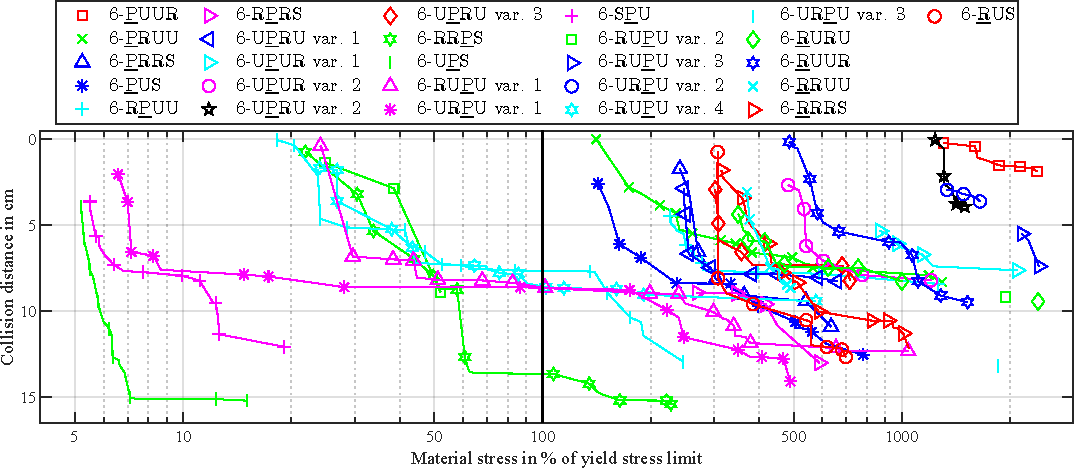
\includegraphics{Figures/lufipkm_pareto_materialstress_colldist_groups_materialstresscolldist_34joints.pdf}
\end{adjustwidth}
\caption[Naval-testbed task: \propername{Pareto} fronts for design-oriented objectives for chains with three and four joints]{\propername{Pareto} fronts for design-oriented objectives for chains with three and four joints with lightweight link dimensioning without the link-design optimization loop.}
\label{fig:lufipkm_pareto_materialstresscolldist_34joints}
\end{figure}

\vspace{-12pt}
\begin{figure}[H]
\begin{adjustwidth}{-\extralength}{0cm}
  \centering
  \graphicspath{{Figures}}
  \input{./Figures/lufipkm_robots1.pdf_tex}
\end{adjustwidth}
\caption{Visualization %
  %
  of valid solutions for the naval-testbed robot from Figure~\ref{fig:lufipkm_pareto_materialstresscolldist_34joints}. The fixed base is at the top, and the moving platform is at the bottom. Red cuboids mark active prismatic joints, and blue cylinders or spheres mark passive joints.}
\label{fig:lufipkm_robots1}
\end{figure}

%
In another run of the optimization, the objectives were selected as the  moving parts' mass (excluding motors and joints, objective~\refl{itm:obj_mass} from Section~\ref{sec:ds_objective}), the actuators' rated power (obj.~\refl{itm:obj_power}), and again, the collision distance (obj.~\refl{itm:obj_colldist}).
Figure~\ref{fig:lufipkm_pareto_power_mass_groups_default_hexapod_and_hexa} shows the \propername{Pareto} diagrams of the first two objectives for the combination of base- and platform-joint alignments for a hexapod (a), a Hexa (b), and a HexaSlide~(c).
The mass is influenced mainly by the length of the links and the force distribution within the structure, as high material stress (resulting from bending moments from levered forces) requires stronger dimensioning.
The Hexa and the HexaSlide have higher stress in Figure~\ref{fig:lufipkm_pareto_materialstresscolldist_34joints}, and also, after the design optimization, a higher moving structural mass than the hexapod.
However, no dominant structure can be stated regarding the neglected mass of the hexapod's moving actuators and the mass difference of less than 10\% (regarding \SI{60} kg).
\begin{figure}[H]
\begin{adjustwidth}{-\extralength}{0cm}
  \centering
  \begin{overpic}
  {Figures/lufipkm_alignment_compare_RUS_UPS.pdf}
  \put(0,1){(\textbf{a})}
  \put(34,1){(\textbf{b})}
  \put(67,1){(\textbf{c})}
  \end{overpic}  
\end{adjustwidth}
\caption{\propername{Pareto} fronts
  for combinations of coupling-joint alignments of selected parallel robots: (\textbf{a}) Hexapod, (\textbf{b}) Hexa, and (\textbf{c}) HexaSlide}
\label{fig:lufipkm_pareto_power_mass_groups_default_hexapod_and_hexa}
\end{figure}

Performing the dimensional synthesis for several coupling-joint alignments without preliminary fixing allows for comparing their performance.
The HexaGlide discussed in Section~\ref{sec:eval_lufi_intro} (6-\underline{P}US with parallel horizontal base coupling, ``p'') does not provide any solutions due to collisions and the limited available installation space.
The actuator's rated power is approx. 20\% lower for the hexapod (\SI{800}{\watt} compared to \SI{1}{\kilo\watt}).
Since a spherical joint is used for the platform joints of the three structures, only pairwise and regular circular distributions are distinguished with two colors in Figure~\ref{fig:lufipkm_pareto_power_mass_groups_default_hexapod_and_hexa}, in contrast to the base joints with nine possible markers.
The pairwise alignment of both base and platform joints (shifted by one) outperforms other possible alignments for all structures.
Thereby, the optimization algorithm obtains the established alignments from the literature without prior specific knowledge, showing the feasibility of the permutational approach for parallel\hl{-}robot synthesis.


Next, all robot structures are compared regarding the three criteria relevant to the mechanical design and technical realization, summarized in the two \propername{Pareto} diagrams in Figure~\ref{fig:lufipkm_pareto_power_mass_groups}.
Only the \propername{Pareto}-dominant coupling-joint alignments are included, as well as the custom hexapod engineering solution from \cite{Fettin2023_M1174} (see Section~\ref{sec:eval_lufi_engsol}) based on the synthesis.
By comparing moving mass and actuator power (upper part in Figure~\ref{fig:lufipkm_pareto_power_mass_groups}), the same robot assemblies as in Figure~\ref{fig:lufipkm_pareto_materialstresscolldist_34joints} are dominant since the necessary stronger link dimensioning of the previously underdimensioned structures increases their mass.
Most of these structures lead to valid solutions, meaning that the link-design optimization found a stronger dimensioning that was also free of self-collisions despite the increased link~diameters.
The total of 40 structures are listed in Figure~\ref{fig:lufipkm_pareto_power_mass_groups}%
%
, as opposed to 26 in Figure~\ref{fig:lufipkm_pareto_materialstresscolldist_34joints} and \hl{17} in Figure~\ref{fig:lufipkm_pareto_materialstresscolldist_56joints}, with only a few with stress below 100\%. %

The collision criterion is investigated in the lower part of Figure~\ref{fig:lufipkm_pareto_power_mass_groups}.
The dominance of the hexapod becomes visible for this task, as {it} provides the largest possible distances between the leg chains due to its compact construction.
This also presents a safety margin for motion outside of the prescribed workspace and leaves room for detailed construction since collision bodies for the actuators are not included in the simplified model in the synthesis.
For the design of the system, not only the actuators' rated power but also their torque and speed have to be compared to select from catalogs of existing motor-gear combinations.
Together with the collision distance, these objectives (numbers~\refl{itm:obj_maxactforce} and \refl{itm:obj_maxactvelo} in Section~\ref{sec:ds_objective}) were optimized in another run, resulting in \propername{Pareto} diagrams in \mbox{Figures~\ref{fig:lufipkm_pareto_linkdiam_colldist}--\ref{fig:lufipkm_pareto_motordiagram_revolute}} in the appendix.
For prismatic actuation, these drive-train characteristics constitute one dense \propername{Pareto} front, showing an equivalence of most structures regarding these criteria, which does not hold for revolute actuation.
The stronger dimensioning of some of the structures as \hl{the} result of the design optimization is visible as well (Figure~\ref{fig:lufipkm_pareto_linkdiam_colldist} and Tables~\ref{tab:lufipkm_results_pris} and~\ref{tab:lufipkm_results_rev}). %
Further robot sketches (Figures~\ref{fig:lufipkm_robots2}--\ref{fig:lufipkm_robots4}) and tables with characteristic values and dimensional parameters (Tables~\ref{tab:lufipkm_results_pris}--\ref{tab:lufipkm_results_rev_dh}) are given in Appendix~\ref{sec:app_lufipkm} for compactness.

\begin{figure}[H]
\begin{adjustwidth}{-\extralength}{0cm}
  \centering
  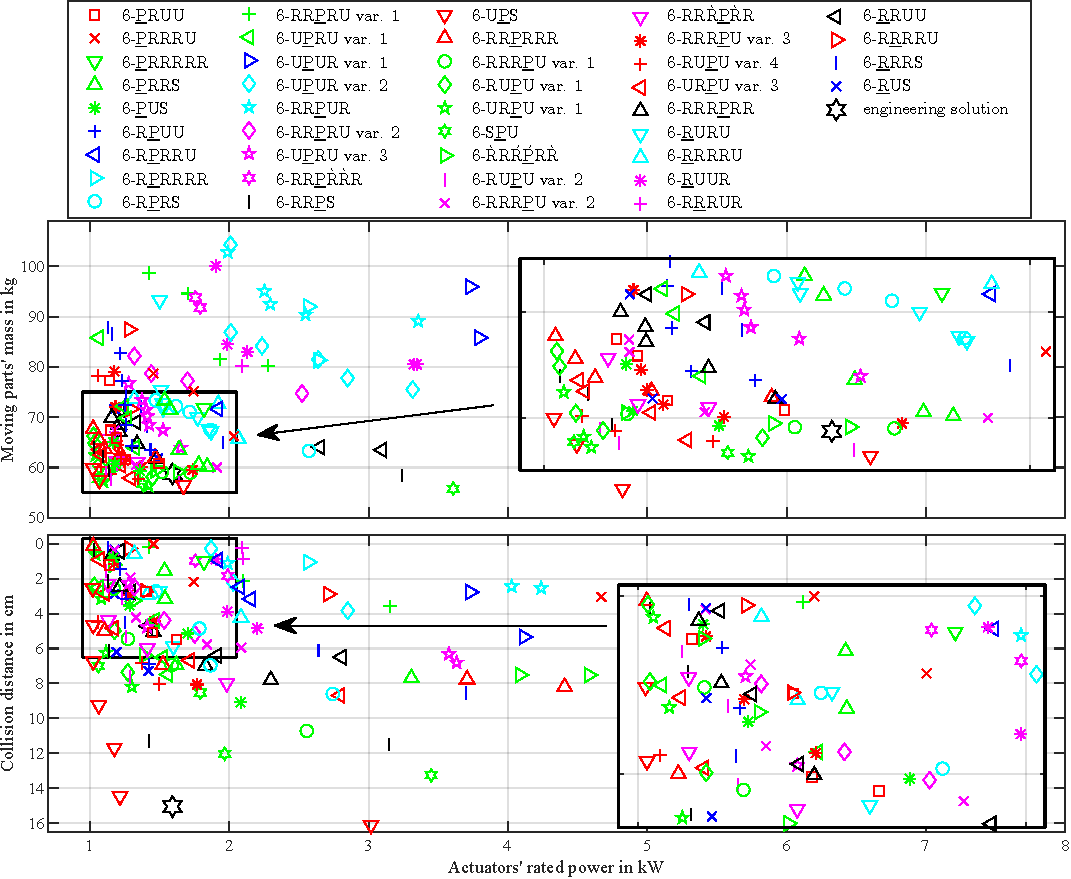
\includegraphics{Figures/lufipkm_pareto_3obj_combined.pdf}
\end{adjustwidth}
\caption{Grouped \propername{Pareto} fronts of all results of the naval-testbed robot.}
\label{fig:lufipkm_pareto_power_mass_groups}
\end{figure}

\subsection{Engineering Solution}
\label{sec:eval_lufi_engsol}

A hexapod was selected in \cite{Fettin2023_M1174} as the most feasible solution for the task.
The final dimensioning was determined based on several runs of the dimensional synthesis and as a compromise solution for multiple objectives (force, velocity, collision, precision, workspace, stiffness, workspace size) and computed for the 3D \propername{Pareto} front of the synthesis with objectives of force, velocity, and collision distance.
The workspace volume was evaluated by a discretization approach from \cite{TartariFilhoCab2005,GharahsoflooRah2015}, which is not feasible to be performed within the dimensional synthesis due to the computation time. 
The objectives were normalized to their best possible value and weighted using a paired comparison based on economic, practical, and task considerations.
Therefore, the solution is not dominant in Figures \ref{fig:lufipkm_pareto_power_mass_groups}, \ref{fig:lufipkm_pareto_motordiagram_prismatic}, and \ref{fig:lufipkm_pareto_motordiagram_revolute}, {i.e., it is above the \propername{Pareto} front for the 6-U\underline{P}S.}
An overview of the resulting construction is given in Figure~\ref{fig:lufipkm_engineering}.
The geometric parameters and performance characteristics are shown in the last row of appendix Table~\ref{tab:lufipkm_results_pris}, together with values for other structures.

\vspace{-2pt}
\begin{figure}[H]
\begin{adjustwidth}{-\extralength}{0cm}
  \centering
  \graphicspath{{Figures}}
  \input{./Figures/lufipkm_engsol.pdf_tex}
\end{adjustwidth}
\caption{\hl{Details} of the engineering solution; modified from \cite{Fettin2023_M1174}: (\textbf{a}) leg chain (modified from the catalog ``Electromechanical cylinders EMC'' from Bosch Rexroth AG, Lohr am Main, Germany), (\textbf{b}) spherical joint, (\textbf{c}) universal joint (derived from a CAD file of Elso Elbe GmbH \& Co. KG., Hofheim, Germany), (\textbf{d}) hexapod assembly, (\textbf{e}) moving platform, and (\textbf{f}) fixed base.} %
\label{fig:lufipkm_engineering}
\end{figure}

The found structure (cf. Figure~\ref{fig:lufipkm_engineering}d) is a classical hexapod with pairwise alignments of base- and platform-coupling joints with correspondence shifted by one.
%
Electric lifting cylinders based on a spindle and axis-parallel motor alignment  (cf. Figure~\ref{fig:lufipkm_engineering}a) were used directly for the leg chains, dimensioned regarding the minimal and maximal stroke and the required actuator force and speed from the simulation.
Further specific constraints had to be respected (i.e., inability to use the full stroke under load, cylinder length offset to account for joint and adapter dimensions, and ability to support the total system's mass when the robot stands on the mobile platform).
The same standard universal joints (cf. Figure~\ref{fig:lufipkm_engineering}c) were used for the base and platform coupling due to their availability.
An additional revolute joint was added for the kinematic spherical joint (cf. Figure~\ref{fig:lufipkm_engineering}b), and no ball-and-socket joints were used.
%
A tilt adapter for the base- and platform-coupling joints (cf. \SI{21.5}{\degree} in Figure~\ref{fig:lufipkm_engineering}e) was chosen to reduce the joints' tilting angle to \SI{31}{\degree} (of maximal \SI{35}{\degree}) during the reference motion.
The base-frame design (Figure~\ref{fig:lufipkm_engineering}f) fulfills the requirements regarding interface compatibility, transportability, and parts availability.

The mechanical design of the base showed that the resulting parameter for base-rotation offset is not feasible, and a parallel alignment of one base-joint pair to the frame's edge by $\varphi_{\mathrm{b},z}{=}\SI{180}{\degree}$ was used instead (Figure~\ref{fig:lufipkm_engineering}f), which only led to negligible degradation of the system performance.
The same holds for the platform rotation offset parameter $\varphi_{\mathrm{p},z}$, which now can be set in discrete values of \SI{15}{\degree} with the circular flange  (Figure~\ref{fig:lufipkm_engineering}e) and makes the robot adaptable to different tasks and ship models.


\subsection{Summary of the Case Study}
\label{sec:eval_lufi_summary}


%
%
%
%
%
%

For the naval-testbed task, the combined structural and dimensional synthesis found valid solutions for the majority of available kinematic structures.
The best performance of the design-oriented objectives was achieved by widely-used structures with three joints per chain.
For these standard solutions (see, e.g., \cite{FrindtKreHes2010}), the framework presents an efficient approach for dimensional synthesis.
%
Other solutions were not able to outperform the standard designs. 
The reasons are the rather nonrestrictive ratio of workspace to installation space and the moderate required tilting angles already achievable by the hexapod. %
Furthermore, the payload produces high bending moments for structures with multiple joints and longer~levers.
%

However, results for structures with more joints are still feasible regarding their performance despite their high design complexity.
The acceptable computational effort shows the \emph{feasibility of the approach for the link-design optimization}, which had to be employed for the multi-joint leg chains to obtain valid solutions.
%
The case study further indicates that after some iterations of the requirements and the synthesis results, the kinematic structure and the drive characteristics were a helpful basis for the design and construction of a robot prototype within the time limitation of a master's thesis.

%
%
%
%

After exploring the diversity of parallel robots with 3T3R end-effector DoFs that the proposed synthesis framework can produce, the subsequent case study focuses on robots with reduced mobility and functional redundancy. An example of using functional redundancy with 3T3R robots with the framework is given in \cite{SterneckFetSch2023}.


%
%
%

\section{Translational Parallel Handling Robots with Arbitrary Planar Rotation}
\label{sec:eval_handlingfreerotation}


%
%
%
%
%
%
%
%

A general handling task is taken as a second case study to investigate structures with 3T0R and 3T1R motion exemplarily.
Arbitrary planar rotation is allowed in the 3T0R task, which produces functional redundancy for 3T1R PRs.
The inverse-kinematics model for this case used in the dimensional synthesis is elaborated on in \cite{Schappler2022_ARK3T1R}.
The case study presents a simulative investigation without reference to an actual robot prototype, unlike in the previous section.
A similar evaluation has been published in \cite{Schappler2022_ARK3T1R} in preliminary form.
In Section~\ref{sec:eval_handling_task}, the requirements, based on the paper \cite{PrauseChaCor2015}, are summarized and formalized within the synthesis framework.
The results are introduced in Section~\ref{sec:eval_handling_results}, followed by the evaluation of functional redundancy in Sections~\ref{sec:eval_handling_results_taskred}--\ref{sec:eval_handling_results_taskred_general}, a comparison to the reference work~\cite{PrauseChaCor2015} in Section~\ref{sec:eval_handling_results_reference_comparison} and the summary in Section~\ref{sec:eval_handling_summary}. %
%


%
%
%
%
%
%
%
%
%


\subsection{Task Requirements}
\label{sec:eval_handling_task}


%
%
%
%
%
%
%
%
%

By reproducing the requirements of the case study from \cite{PrauseChaCor2015}, a validation of this thesis' synthesis framework against the one from \cite{Prause2016} is performed (cf. Section~\ref{sec:ds_combstructgeomsynth}).
The requirements are summarized in Table~\ref{tab:handling_constraints}.
\emph{The task} is specified as a \emph{reachable cuboid workspace} of \SI{200}{\milli\metre} $\times$ \SI{200}{\milli\metre} $\times$ \SI{100}{\milli\metre}.
A visualization is given in Figure~\ref{fig:handlingpkm_robots_selection} with some of the robot structures.
By sampling each dimension with three values, 27 \emph{reference points} are defined. 
The orientation is not specified for 3T1R robots, which permits choosing it by~optimization.

\begin{figure}[H]
  \begin{adjustwidth}{-\extralength}{0cm}
    \centering
    \graphicspath{{Figures}}
    \input{./Figures/handlingpkm_robots_selection.pdf_tex}
  \end{adjustwidth}
  \caption{Visualization %
  %
    of selected results for the handling task from the \propername{Pareto} diagrams in Figure~\ref{fig:handlingpkm_pareto}.}
  \label{fig:handlingpkm_robots_selection}
\end{figure}



\newcounter{handlingconstraints}
\begin{table}[H]
  \caption[Constraints and parameter limits for the handling task]{Constraints and parameter limits for the handling task with reference to numbers in Section~\ref{sec:materials}}
  \begin{adjustwidth}{-\extralength}{0cm}
    \centering
    \label{tab:handling_constraints}	
    \begin{tabularx}{\fulllength}{CcCc}
      \toprule
      \textbf{\#} & \textbf{Constraint} & \textbf{Section~\ref{sec:ds_constraints}} &  \textbf{Value} \\
      \midrule
      \refstepcounter{handlingconstraints}\thehandlingconstraints\label{handlingconstr:installspace} & \makecell{installation space (depending\\ on joint index in the chain)} & no.~\ref{itm:constr_installspace} & \makecell{joints 1--3 not above lower workspace limit,\\ joints 4--5 not above upper workspace limit} \\		
      \midrule
      \refstepcounter{handlingconstraints}\thehandlingconstraints\label{handlingconstr:prismaticrange} & prismatic joint stroke length & no.~\ref{itm:constr_jointrange}  & max. \SI{400}{\milli\metre} \\
      \midrule
      \refstepcounter{handlingconstraints}\thehandlingconstraints\label{handlingconstr:legchainlength} & length of a leg chain & no.~\ref{itm:constr_jointrange} & max. \SI{1000}{\milli\metre} \\
      \midrule
      \refstepcounter{handlingconstraints}\thehandlingconstraints\label{handlingconstr:baselim} & base diameter & no.~\ref{itm:constr_param_radius}  &  200--1000 mm \\
      \midrule
      \refstepcounter{handlingconstraints}\thehandlingconstraints\label{handlingconstr:plflim} & platform diameter & no.~\ref{itm:constr_param_radius} &  200--1000 mm, smaller than base \\	
      \midrule
      \refstepcounter{handlingconstraints}\thehandlingconstraints\label{handlingconstr:poserr} & precision (position error) & no.~\ref{itm:constr_obj} &  max. \SI{0.5}{\milli\metre} (for objective~\ref{itm:obj_poserr} in Section~\ref{sec:ds_objective})\\
      \midrule
      \refstepcounter{handlingconstraints}\thehandlingconstraints\label{handlingconstr:condition} & \propername{Jacobian} condition number  & no.~\ref{itm:constr_ik_sing} &  \gape{max. $10^4$ (IK and manipulator \propername{Jacobian})}\\
      \midrule
      & \textbf{Parameter} & \textbf{Section~\ref{sec:dimsynth_optvars}} &  \textbf{Value} \\
      \midrule
      \refstepcounter{handlingconstraints}\thehandlingconstraints\label{handlingconstr:baseposition_z} & vertical base position in $\rovec{\indks{W}}{0}$ & no.~\ref{itm:param_basepos} & 1--0.1 m below the task \\
      \midrule
      \refstepcounter{handlingconstraints}\thehandlingconstraints\label{handlingconstr:baseposition_xy} & base position in $x$-$y$-plane & no.~\ref{itm:param_basepos} & 0 (no optimization) \\
      \midrule
      \refstepcounter{handlingconstraints}\thehandlingconstraints\label{handlingconstr:param_baseori} & \gape{base rotation $\rotmat{\indks{W}}{0}$} & no.~\ref{itm:param_baseori} & $\varphi_{\mathrm{b},x}~{=}~\varphi_{\mathrm{b},y}~{=}~0$ and $\varphi_{\mathrm{b},z}{\in}[-\SI{180}{\degree},\SI{180}{\degree}]$\\
      \midrule
      \refstepcounter{handlingconstraints}\thehandlingconstraints\label{handlingconstr:param_basejointincl} & base-joint inclination $\gamma_{\mathrm{b}}$ & no.~\ref{itm:constr_param_inclination} & $\SI{5}{\degree} < \gamma_{\mathrm{b}} < \SI{30}{\degree}$ (for conic alignment)\\
      \midrule
      \refstepcounter{handlingconstraints}\thehandlingconstraints\label{handlingconstr:ee_translation} & end-effector translation $\rovec{\indks{P}}{\indks{E}}$ & no.~\ref{itm:param_eepos} & [0,\,0,\,0] (no optimization) \\	
      \midrule
      \refstepcounter{handlingconstraints}\thehandlingconstraints\label{handlingconstr:param_eeori} & \gape{end-effector orientation $\rotmat{\indks{P}}{\indks{{E}}}$} & no.~\ref{itm:param_eeori} & $\varphi_{\mathrm{p},x}=\varphi_{\mathrm{p},y}=\varphi_{\mathrm{p},z}=0$ (no opt.)\\
      \midrule
      & \textbf{Load} &  &  \textbf{Value} \\
      \midrule
      \refstepcounter{handlingconstraints}\thehandlingconstraints\label{handlingconstr:forces} & maximal external forces &  &  \gape{$\ortvek{W}{f}{\transp}{\mathrm{ext}}=$ [2,\,2,\,$-$10] \SI{}{\newton}}  \\
      \bottomrule
    \end{tabularx}
  \end{adjustwidth}
\end{table}

The combined structural and dimensional synthesis in \cite{PrauseChaCor2015} is based on the 27 reference points, and results for 3T0R PRs with prismatic actuation are obtained using a single-objective optimization. %
There, a detailed investigation of the best parameterization for all structures is performed with a finer discretization of \SI{10}{\milli\metre} in each dimension and, thereby, 4851 points.
Since the proposed framework can handle this complexity, a \emph{reference path} connecting the 4851 points in a zigzag motion (by the same number of samples) is used directly within the synthesis of this study after the check of the 27 reference points.
Thereby, the risk of unreachable parts within the workspace decreases.
For 3T1R robots, dynamic programming (cf. \cite{Schappler2023_ICINCOLNEE}) is used for optimizing the redundant rotational \hl{DoF} with twelve stages and five states %
and a limitation of $\pm$\SI{60}{\degree} around the initial value, resulting from the IK optimization.

Only the force transmission, without statics or dynamics, is considered, as in \cite{PrauseChaCor2015}.
The \emph{robot and payload mass are neglected}, which allows the use of the simplified \emph{trajectory} with discontinuous velocity and acceleration profiles by numeric differentiation.
The actuator force is computed based on a given external force (corresponding to a payload of \SI{1} kg, cf. row~\ref{handlingconstr:forces} in Table~\ref{tab:handling_constraints}) and used as an objective (number~\ref{itm:obj_maxactforce} in Section~\ref{sec:ds_objective}), as in \cite{PrauseChaCor2015}.
As a second additional objective (number~\ref{itm:obj_installspace} in Section~\ref{sec:ds_objective}), the installation space is used to be able to select robots with a good ratio of (fixed) workspace to (optimized) installation space.
The precision (number~\ref{itm:obj_poserr} in Section~\ref{sec:ds_objective}) was selected as a third criterion for further exploration of the solution space as it conflicts with the actuator force by lever effects.


\begin{figure}[H]
  \begin{adjustwidth}{-\extralength}{0cm}
    \centering
    \begin{overpic}
      {Figures/handlingpkm_pareto_actforce_installspace_groups_default_prismatic.pdf}
      \put(0,0){(\textbf{a})}
    \end{overpic}\\[5mm]
    \begin{overpic}
      {Figures/handlingpkm_pareto_actforce_installspace_groups_default_revolute.pdf}
      \put(0,0){(\textbf{b})}
    \end{overpic}
  \end{adjustwidth}
  \caption{\propername{Pareto} fronts for robots with (\textbf{a}) prismatic and (\textbf{b}) revolute actuation. The notation of \cite{KongGos2007} is used for distinguishing kinematic structures, where {two} \`R denote two parallel revolute joints and \'R denotes {a} joint with a different axis.
    {In addition to \cite{KongGos2007}, prismatic joints with an axis parallel to a revolute \`R joint are denoted by \`P.}}
  \label{fig:handlingpkm_pareto}
\end{figure}
Several geometric \emph{constraints} are set to increase the practicability of the solutions. 
A floor-mounted PR is assumed to simplify the visualizations contrary to the more practical existing ceiling-mounted robots.
The robot structure should be below the workspace (row~\ref{handlingconstr:installspace}) to avoid impractical crane-like designs.
Further constraints are taken from \cite{PrauseChaCor2015}, such as a limited prismatic joint stroke (row~\ref{handlingconstr:prismaticrange}), chain length (row~\ref{handlingconstr:legchainlength}), and base and platform diameters (rows~\ref{handlingconstr:baselim} and~\ref{handlingconstr:plflim}).
The required joint-coordinate range of prismatic joints in the chain (realized by lifting cylinders) results in 400--800 mm by constraint no.~\ref{itm:constr_prismaticcylinder} from Section~\ref{sec:ds_constraints}.
To avoid singularities and to obtain feasible handling performance, e.g., in industrial pick-and-place tasks, the end-effector precision (row~\ref{handlingconstr:poserr}) was additionally limited to \SI{500}{\micro\metre}, which is {achieved by} all results from \cite{PrauseChaCor2015} {(Figure~\ref{fig:handlingpkm_boxplot_PrauseChaCor2015}d in Appendix~\ref{sec:app_handlingpkm})} and %
%
does not deteriorate the comparability.
The encoder error of \SI{52}{\micro\metre} from \cite{PrauseChaCor2015} was used for prismatic actuation and \SI{7}{\arcsecond} from \cite{HeidenheinEncoder} for revolute actuation.
For further exclusion of near-singular PRs (\mbox{types~I and~II}), \propername{Jacobian} condition-number limits are set (row~\ref{handlingconstr:condition}).
The robot base is assumed below the center of the workspace (rows~\ref{handlingconstr:baseposition_z} and~\ref{handlingconstr:baseposition_xy}) with further optimization of the base rotation (row~\ref{handlingconstr:param_baseori}).
No end-effector transformation is assumed (rows~\ref{handlingconstr:ee_translation} and~\ref{handlingconstr:param_eeori}), and only an offset distance is used for visualization, e.g., in Figure~\ref{fig:handlingpkm_robots_selection}.

In \cite{PrauseChaCor2015}, only robots with tangential (``triangular'') and conical (``star-shaped'') \emph{base-joint alignment} are considered as showcases.
This restriction is lifted in the following, and all other structures (radial and vertical base joints) are allowed to increase the number of results and show the variety of produced solutions by the proposed framework.
Only the restriction on the conical base joints' elevation of \cite{PrauseChaCor2015} is maintained (row~\ref{handlingconstr:param_basejointincl}) for~compatibility.


The synthesis is performed for all 3T0R and 3T1R PRs from a previous structural synthesis {with actuation} of the first revolute or single prismatic joint.
In total, 329 variants (combinations of leg chains and base- and platform-coupling\hl{-}joint alignments) are investigated, 239 for 3T0R and 90 for 3T1R.
Of these, 226 match the requirements (200 for 3T0R and 26 for 3T1R).
The results are summarized into 36 groups of 3T0R (25 prismatic and 11 revolute actuation) and 12 groups of 3T1R (5 prismatic, 7 revolute actuation) by their respective leg chain.
The results for all coupling-joint alignments for one leg chain are summarized into one \propername{Pareto} front, similar to the case study in Section~\ref{sec:eval_water}.

The particle swarm optimization for 7 to 13 parameters (depending on the structure) is configured similarly as before, with 400 individuals and a time limit of \SI{10}{\hour} with a computation time of up to 20--40 s for 3T0R and \SI{2}{\minute} for 3T1R robots, depending on the abortion due to constraint violation.
The longer computation time for 3T1R robots results from the more complex model (one additional chain), more possibility for assembly modes, and especially, the redundancy resolution.
Several optimization iterations are performed in which constraints are added and refined, and intermediate results are taken as initial values for the successive iterations.

\subsection{Overview of the Synthesis Results}
\label{sec:eval_handling_results}

%
%
%
%
%
%


The optimization results are depicted in Figure~\ref{fig:handlingpkm_pareto} in \propername{Pareto} fronts separately for prismatic and revolute actuation due to the different units and clarity.
Four exemplary robot structures are shown in Figure~\ref{fig:handlingpkm_robots_selection}.
The remainder of the structures are visualized in Appendix~\ref{sec:app_handlingpkm} in Figures~\ref{fig:handlingpkm_robots_3T0R_rev1}--\ref{fig:handlingpkm_robots_reference} with parameters in Tables~\ref{tab:handlingpkm_results_pris}--\ref{tab:handlingpkm_results_rev_dh}.

For \emph{prismatic actuation} in Figure~\ref{fig:handlingpkm_pareto}a, many different structures show a comparably good performance; however, the
\hyperrefl{restabrow:P3PRRRR7V1GxPxA1}{3-\underline{P}{U}{R}{R}} (Figure~\ref{fig:handlingpkm_robots_3T0R_pris1}h),  \hyperrefl{restabrow:P3PRRRR8V1GxPxA1}{3-\underline{P}{U}{U}} (linear Delta, Figure~\ref{fig:handlingpkm_robots_selection}c), and \hyperrefl{restabrow:P3PRRRR8V2GxPxA1}{3-\underline{P}RRU} (variant 2, Figure~\ref{fig:handlingpkm_robots_3T0R_pris1}k) clearly outperform the other solutions regarding the selected criteria.
The \hyperrefl{restabrow:P3PRRRR7GxPxA1}{3-\underline{P}{R}{\`R}{\`R}{\`R}} (Figure~\ref{fig:handlingpkm_robots_3T0R_pris1}g) and \hyperrefl{restabrow:P3PRRRR8GxPxA1}{3-\underline{\`P}{\`R}{\'R}{\'R}{\`R}} (Figure~\ref{fig:handlingpkm_robots_3T0R_pris1}i) show similar performance, as they correspond to the same robots but with universal joints expanded to single revolute joints.
The 3T1R structures require a significantly higher actuator force of about \SI{10}{\newton} (e.g.,~\hyperrefl{restabrow:P3RPRRR8V3GxPxA2}{4-{\`R}\underline{P}{\`R}{\'R}{\'R}}, Figure~\ref{fig:handlingpkm_robots_selection}d) compared to \SI{4}{\newton} (Figure~\ref{fig:handlingpkm_pareto}a) for a similar installation space.


For the \emph{revolute actuation} in Figure~\ref{fig:handlingpkm_pareto}b, the \hyperrefl{restabrow:P3RRRRR6V1GxPxA1}{3-\underline{R}{U}{R}{R}} (Figure~\ref{fig:handlingpkm_robots_3T0R_rev1}g) performs best, followed by the Delta robot structure (\hyperrefl{restabrow:P3RRRRR10V1GxPxA1}{3-\underline{R}{U}{U}}, Figure~\ref{fig:handlingpkm_robots_selection}a) and variants thereof.
The Delta's base-joint alignment is chosen unconventionally by a radial drive axis.
The ability of this alignment to support the established Delta robot construction using a spatial parallelogram needs further investigation before eventual realization.
The relative disadvantage of 3T1R structures is similar to prismatic actuation of about 100\% regarding the actuator force/torque of the best 3T0R structure.
The 3T1R \hyperrefl{restabrow:P4RRRRR10V1GxPxA1}{4-\underline{R}{U}{U}} (Figure~\ref{fig:handlingpkm_robots_selection}b), for instance, and the \hyperrefl{restabrow:P4RRRRR5V1GxPxA1}{4-\underline{R}{R}{U}{R}} (Figure~\ref{fig:handlingpkm_robots_3T1R_rev}e), e.g., require \SI{3}{\newton\metre} and \SI{2}{\newton\metre} actuator torque compared to \SI{1}{\newton\metre} for the 3T0R \hyperrefl{restabrow:P3RRRRR6V1GxPxA1}{3-\underline{R}{U}{R}{R}}.


\subsection{Comparison to Results from the Literature and Evaluation of the Framework}
\label{sec:eval_handling_results_reference_comparison}

The structures from \cite{PrauseChaCor2015} are evaluated in Figure~\ref{fig:handlingpkm_pareto}a as an additional benchmark if they exist in the database.
Structures with both prismatic (P) and cylindrical (C) joints are omitted since this corresponds to two prismatic DoFs (one passive) within one leg chain.
%
A rather exact reproduction of the actuator forces from \cite{PrauseChaCor2015} was possible for the 3-\underline{C}RR, 3-\underline{P}UU, and 3-U\underline{P}U using the parameters from the paper, as is visible in a comparison of the box plots from \cite{PrauseChaCor2015}, cf. Figure~\ref{fig:handlingpkm_boxplot_PrauseChaCor2015}.
For the 3-\underline{C}UR and 3-\underline{C}RU, the values were in the same range but with a different distribution over the 4851 trajectory samples.
The difference is already contained within the \propername{Jacobian}, which differs between the robot assembly modes, visible in Figure~\ref{fig:handlingpkm_boxplot_PrauseChaCor2015}e--f.
In conclusion, the \emph{kinetostatic model} is likely consistent.
Still, the reference's collision model (if any) and the selection strategy of the assembly mode may explain the deviation using the same kinematic parameters.
%
%

The markers from \cite{PrauseChaCor2015} are dominated by the corresponding \propername{Pareto} fronts (using the same marker symbol but a different color).
Due to the complexity of the \emph{optimization problem}, a possible reason is hard to determine.
The additional use of the reference trajectory does not explain the difference  from \cite{PrauseChaCor2015}, where results are only based on the 27 reference points, as the optimization only based on these 27 reference points leads to qualitatively similar results as Figure~\ref{fig:handlingpkm_pareto}a, shown in appendix Figure~\ref{fig:handlingpkm_pareto_prismatic_onlypoints}.
Next to the differences mentioned above, one other reason could be an undocumented further constraint in the paper or the underlying framework of the PhD thesis \cite{Prause2016}.
An influence that is not less likely is the insufficient exploration ability of the employed single-objective genetic algorithm from \cite{MatlabGOT} instead of the PSO, which was also observed (for the multi-objective variant) in the case study~\cite{SchapplerJahRaaOrt2022}.


\subsection{Evaluation of Functional Redundancy of 3T1R Parallel Robots}
\label{sec:eval_handling_results_taskred}

Although symmetric 3T1R PRs do not reach as low actuator forces as their 3T0R counterparts, their principal operational capability presents an interesting result compared to the state of the art, where mostly theoretical structures are shown.
They benefit from the redundancy resolution using dynamic programming (see \cite{Schappler2023_ICINCOLNEE}). %

In Figure~\ref{fig:handlingpkm_perfmap_traj}b, an illustrative performance map is given for the \hyperrefl{restabrow:P4RPRRR8V2GxPxA2}{4-{R}\underline{P}{U}{R}} (Figure~\ref{fig:handlingpkm_robots_3T1R_pris}\,b).
This heat-map representation of the redundant degree of freedom over the trajectory was introduced by Wenger (see \cite{RevelesWenoth2016}) and is discussed in \cite{Schappler2023_ICINCOLNEE} in more detail.
The actuator-force representation in the map color corresponds to the objective of the IK optimization. 
It provides a direct interpretation in this case study since only the transmission of the given external force is considered, and rigid-body dynamics are neglected.
Within the optimization of the planar rotation coordinate, the maximal force of any of the actuators is minimized to 
5.3--12.2 N by avoiding orientations with higher forces. %
The upper bound is taken as objective (number~\ref{itm:obj_maxactforce} in Section~\ref{sec:ds_objective}) in Figure~\ref{fig:handlingpkm_pareto}.
For reference, the position trajectory is given in Figure~\ref{fig:handlingpkm_perfmap_traj}a, showing the zigzag motion of the $x$ and $y$ coordinates while ascending in the $z$ coordinate and, thereby, sampling the cuboid workspace.
The actuator-force/-torque performance maps of the other 3T1R PRs are given in appendix Figure~\ref{fig:handlingpkm_perfmaps_multi_actforce_pris} and~\ref{fig:handlingpkm_perfmaps_multi_actforce_rev}.
There, avoiding constraint violations (singularities, collisions, accuracy) dominates the force objective within the motion due to the relatively homogeneous pose-independent transmission ratio of the given external force (regarding the most-stressed actuator).
The evaluation already shows that the redundancy-resolution scheme from \cite{Schappler2023_ICINCOLNEE} also provides plausible results for 3T1R PRs regarding the optimality of the trajectory of the redundant~coordinate. 

\vspace{3pt}
\begin{figure}[H]
  \centering %
  \begin{adjustwidth}{-\extralength}{0cm}
    \begin{overpic}%
      {Figures/handlingpkm_trajectory.pdf} %
      \put(107,0){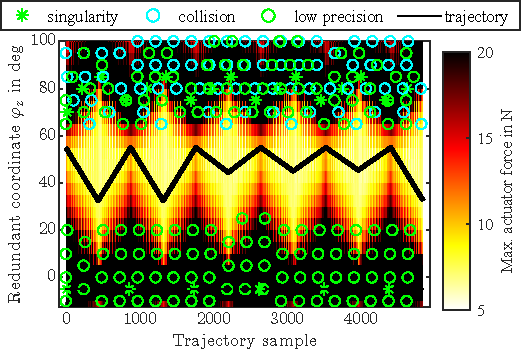
\includegraphics{Figures/handlingpkm_perfmaps_detail_P4RPRRR8V2G_actforce_maxactforce.pdf}} %
      \put(0,0){(\textbf{a})}
      \put(107,0){(\textbf{b})}
    \end{overpic}
  \end{adjustwidth}
  \caption{Trajectory
    of end-effector position (\textbf{a}) and of the planar rotation (redundant coordinate) within the force performance map with markers for constraint violation (\textbf{b}) for the 4-{R}\underline{P}{U}{R}.} %
  \label{fig:handlingpkm_perfmap_traj}
\end{figure} 

\textls[15]{The inspection of performance maps for other criteria in Figures~\ref{fig:handlingpkm_perfmaps_multi_poserr_pris}--\ref{fig:handlingpkm_perfmaps_multi_condikjac_rev} shows possible disadvantages of the symmetric 3T1R PRs compared to 3T0R PRs, even though all constraints are met within the results of the \propername{Pareto} front.
  The position error is much higher for prismatic actuation, except for the  \hyperrefl{restabrow:P4PRRRR6V1GxPxA1}{4-\underline{P}{R}{U}{R}} (Figure~\ref{fig:handlingpkm_robots_3T1R_pris}a), cf.~Figure~\ref{fig:handlingpkm_perfmaps_multi_poserr_pris}a.
  Many 3T1R PRs with revolute actuation exhibit IK singularities within the workspace, which is not possible to detect or avoid numerically with the \SI{10}{\milli\metre} trajectory sampling and the chosen approach of discretely evaluating the condition number, as, e.g., visible in Figure \ref{fig:handlingpkm_perfmaps_multi_condikjac_rev}b,f,g).
  Therefore, special attention must be paid to this aspect to investigate the structures further.}


The objective of the inverse kinematics influences the motion of the platform rotation, provided that the constraints leave sufficient space for optimization.
An example of the trajectories resulting from different IK objectives is given in Figure~\ref{fig:handlingpkm_pareto_compare_ik_obj}a for a parameterization of the \hyperrefl{restabrow:P4RPRRR8V2GxPxA2}{4-{R}\underline{P}{U}{R}} with radially aligned base-coupling joints (unlike in Figure~\ref{fig:handlingpkm_robots_3T1R_pris}b).
The precision is chosen as map color as it also highlights singularities.
Repeating the variation of the IK objective for each point of the robot's \propername{Pareto} front from the optimization (termed ``heuristic'') and evaluating the objective functions leads to a new \propername{Pareto} front for each of the IK objectives, shown in Figure~\ref{fig:handlingpkm_pareto_compare_ik_obj}b--c.
Therefore, the selection of the IK objective indirectly influences the performance of the dimensional synthesis.
Using the same objectives for the IK redundancy resolution and the dimensional synthesis provides the most promising results and corresponds best to the principle of bilevel optimization.
In the specific example of Figure~\ref{fig:handlingpkm_pareto_compare_ik_obj}b, the precision can be reduced by approximately 5\% against the constant-orientation case and 10\% against the heuristic approach of a weighted sum of several objectives, depending on the objectives and constraints of the dimensional synthesis.
The approach does not provide significant improvement for the installation-space objective, as visible in Figure~\ref{fig:handlingpkm_pareto_compare_ik_obj}c.
Other examples (case studies or robots) show qualitatively similar results.
The extent of possible improvement depends on the objectives of the dimensional synthesis and the IK settings that were used to obtain the results, as well as on the robot and task~requirements.

\begin{figure}[H]
  \begin{adjustwidth}{-\extralength}{0cm}
    \begin{overpic}%
      {Figures/handlingpkm_perfmap_compare_ik_obj_P4RPRRR8V2G3P1A1_p1.pdf} %
      \put(101,0){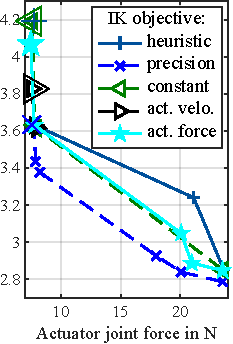
\includegraphics{Figures/handlingpkm_pareto_actforce_positionerror_compare_P4RPRRR8V2G3P1A1_p1.pdf}} %
      \put(142,0){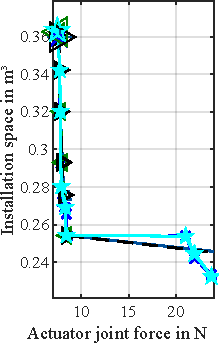
\includegraphics{Figures/handlingpkm_pareto_actforce_installspace_compare_P4RPRRR8V2G3P1A1_p1.pdf}}
      \put(0,2){(\textbf{a})}
      \put(98,2){(\textbf{b})}
      \put(140,2){(\textbf{c})}
    \end{overpic}
  \end{adjustwidth}
  \caption{Redundant-coordinate trajectory (\textbf{a}) and \propername{Pareto} fronts (\textbf{b},\textbf{c}) for another 4-{R}\underline{P}{U}{R} structure based on the same parameters with different inverse-kinematics optimization objectives. The method legend in (\textbf{b}) holds for all (\textbf{a}--\textbf{c}). Large markers in~(\textbf{b},\textbf{c}) represent parameters for the performance map in~(\textbf{a}).} %
  \label{fig:handlingpkm_pareto_compare_ik_obj}
\end{figure} 


%
%
%

%
%


\subsection{Discussion of Redundancy Resolution Within the Dimensional Synthesis}
\label{sec:eval_handling_results_taskred_general}

The downside of possible improvements by redundancy resolution is that the (multi-objective) dimensional synthesis optimization results are based on the (single-objective) redundancy-resolution method.
The performance of the synthesis {with one setting} can then not be obtained by other IK settings.
This overfitting can be avoided by using generic or no IK objectives (e.g., constant orientation or minimal platform motion) with little degree of freedom (e.g., few states in the dynamic programming) at the cost of lower performance in the synthesis objectives.
%
%
%
%
By these results and considerations, the two underlying assumptions of the paper regarding dimensional synthesis and functional redundancy can be addressed: %

%
%
%
%
%
%
\begin{Assumption}
  Optimizing the objective of the dimensional synthesis in an inner-loop redundancy resolution improves the synthesis results in the case of functional redundancy.
\end{Assumption}

%
%
An improvement of the synthesis objective by up to 10\% was shown for some examples.
Therefore, the proposed inner loop  ``\emph{is likely to improve the synthesis results}''. 
As the effect varies, the assumption may not hold in all cases or can not be tested generally (for the complete \propername{Pareto} front, all tasks, and all robot structures).

A thorough statistical evaluation for greater generality would require a metric for comparison of \propername{Pareto} fronts.
This is aggravated by the fact that the density of particles on the front is imbalanced, and gaps in the front are sometimes due to impossibility by constraint violations, sometimes by insufficient exploration.
The true form of the front is thereby unknown and only sampled incompletely by the heuristic optimization algorithm.
%
Quantifying the effect in a single-objective optimization would be easier from a methodological point of view.
However, it would also be less valuable, as a trade-off between multiple objectives has to be found for an actual robot design.
%
This leads to

\begin{Assumption} For a meaningful comparison including functionally redundant robots, the redundancy resolution has to be performed within the dimensional synthesis. Only then can the dominance (outperformance) of one structure compared to another be determined.
\end{Assumption}
%
%
%

\newpage
The redundancy resolution should be used to avoid constraint violations and receive feasible results in the first place.
Without using the redundancy at all, too many particles (i.e., sets of kinematic parameters) would be unnecessarily discarded for constraint violation, which would deteriorate the results.
The assumption can be \emph{argued to be true if redundancy resolution is only defined as avoiding constraint violation} and having no influence otherwise (i.e., leaving the redundant coordinate constant or using some shortest-distance metric for optimization beyond the constraints).

Furthermore, optimizing for a general objective for \emph{the initial poses of the reference trajectory} proved to be a promising approach. %
This may be influenced by the fact that most of the \propername{Pareto}-optimal performance maps could be traversed well with constant orientation, and the performance distribution over the redundant coordinate did not change much.
It can be assumed that this was not induced by the synthesis (i.e., self-fulfilling by overfitting) since the redundancy resolution was also proven to cope with other, more complicated cases.
For the synthesis of other trajectories, %
this could already be different, and the initial pose may have less influence as extensive nullspace motion would be necessary regardless.
%
Thereby, from the results obtained so far, the assumption \emph{is not likely valid for understanding redundancy resolution as initial-pose optimization}.

The assumption also does \emph{not hold when understanding redundancy resolution as optimization within the reference trajectory} since several further assumptions have to hold, depending on the use case.
In multi-objective optimization, the non-redundancy-optimized solution may present a compromise solution, and the optimized solution may be better in one objective but worse in the other objectives and, therefore, not \propername{Pareto}-dominant.
The extent of this effect depends on the selection of objectives and their respective opposition.
Optimizing the inverse kinematics for one objective in the design phase may lead to overfitting, and using the structure later with a different IK objective may present worse results.
Therefore, the priority of the objectives and the aversion to this overfitting would have to be defined beforehand for the assumption to be true without restrictions. %


\subsection{Summary of the Case Study}
\label{sec:eval_handling_summary}

The numerous theoretical results show the efficiency of the synthesis approach for this general 3T0R task. %
The results for functional redundancy show, in principle, that reasonable solutions exist and a comparison is feasible. %
However, the performance of redundant structures is weaker than that of non-redundant. %
The 3T1R structures may still perform better for other objectives, which should be evaluated if a task-specific synthesis is performed.
However, due to the simplicity of the 3T0R structures, the advantage of the 3T1R structures to avoid collisions and singularities may not be relevant since 3T0R robots, such as the Delta robot, do not suffer widely from singularities or self-collisions within the workspace.
%
By direct comparison to the results of \cite{PrauseChaCor2015}, parts of the methodology could be validated for the 3T0R case.



%
\section{Discussion}
\label{sec:discussion}

%


%

%
The results obtained can answer the paper's \emph{research question}: ``How should the optimization problem of the dimensional synthesis be structured if functional redundancy and design optimization are considered?''
%
Solving the problem by nested optimization loops is shown to be feasible due to the reduced number of optimization variables in the single steps.
By this, the most efficient method can be used at each stage of the optimization.
Design optimization and redundancy resolution should be executed consecutively as far as the problem interconnections allow, which holds for the selected evaluation examples. 
%



%



Within this paper, the optimization framework for the dimensional synthesis of parallel robots is explained in detail, focusing on several aspects, {such as a complete description of the optimization problem for later reference in terms of variables, objectives and constraints,} design optimization, and redundancy resolution.
{A comprehensive overview of the literature on dimensional synthesis provides applicable approaches that are further developed for the requirements of this paper.}
%
{The concept of} hierarchical constraints with continuous penalties {presents a general contribution to the state of the art on nonlinear optimization.}
{The field of dimensional synthesis is furthered by promoting} multi-objective particle swarm optimization {with a bilevel strategy} and using the dynamics regressor form for the design optimization.
The extensions lead to improved computational efficiency in contrast to existing methods, {making the combined synthesis practically possible.}

{Further gains in efficiency are possible} in the non-redundant case by using analytic solutions instead of the general numeric iterative approach for solving the inverse-kinematics problem.
{However, this has not yet been implemented} for the parallel\hl{-}robot database due to the large {number} and variety of structures. %
On the other hand, the iterative solution to the inverse-kinematics problem is necessary to perform gradient-descent optimization in the case of functional redundancy, which is used to generate more valid and generally better solutions for dimensional synthesis. %

Several limiting assumptions from the literature regarding included robot structures in the synthesis have been lifted; some more prevent a completely comprehensive robot synthesis.
%
%
The approach of permutational synthesis is also promising for \emph{non-symmetric alignments of coupling joints} for parallel robots with identical leg chains. 
The complexity of the optimization for \emph{non-symmetric parallel robots} (i.e., with different leg chains) should be subject to further investigation, as the robots' performance {(especially in non-symmetric tasks)} may be further improved, as already shown in the literature for some manually designed structures. 
In principle, the proposed framework would be efficient enough to increase the number of structures by one order of magnitude.
Still, the complexity of non-symmetric robots in a geometric permutation could be more extensive than that. %
For such numbers of structures, the optimization algorithm has to be improved by, e.g., exchanging parameter values between different structures, corresponding to sub-populations in the particle-swarm optimization, and more efficient reuse of previous results of other use cases. 
Realizing this would require multiple iterative runs of the optimization or synchronization of the currently independent parallel optimizations.

Another direct application of the developed optimization scheme can be found by lifting the restriction of fully parallel robots by allowing \emph{more than one active joint per leg chain} and reducing the number of legs. 
This step could, in principle, \emph{combine some advantages of serial and parallel robots}, provided that the dimensioning is optimal. 
For instance, the workspace could be larger than that of a parallel robot of comparable size while still being more energy efficient than serial robots by low moving masses.
Concepts for manipulators of this type already exist, but their design was optimized manually or only for one structure.
%
Exploring this relation to both sides presents an interesting research question that requires a \emph{drive-train optimization}, which has not yet been implemented in the proposed framework and would require corresponding component databases or scaling methods already available in the literature.
Serial robots are principally supported by the framework---in the theoretical framework as well as in the implementation.


%
\section{Conclusions}
\label{sec:conclusions}

The ambition of fast computation regarding the large number of structural permutations from a previous structural synthesis characterizes the proposed algorithm extensions for the \emph{dimensional synthesis}.
Compliance with this goal can already be seen by the application within structural synthesis, where several hundred to thousand iterations must be performed for each of the thousands of structural permutations.
The proposed concept of \emph{hierarchical constraints} with \emph{continuous penalties} and \emph{early abortion} has not {yet} been explicitly demonstrated within dimensional synthesis.
In combination with particle swarm optimization, also uncommon in the literature on robot synthesis, fast convergence and good exploration were achieved simultaneously despite the high number of optimization variables.
Additions to the framework regarding reusing results for initial values, also across similar structures, further improved the computational efficiency, which is crucial to solving a task-specific synthesis problem.
Incorporating \emph{design optimization} into the concept was possible by separating independent optimization problems efficiently. %
\emph{Functional redundancy} was integrated similarly, again by following the principle of bilevel optimization, which can be termed nested or \emph{cascaded optimization}. %

%
%
%
%
%
%
%

The ability of the combined structural and dimensional synthesis to generalize on practical problems is shown in two case studies.
%
%
The examples show how to transfer technical requirements to the parameters of the synthesis framework and, used as a template, simplify solving new problems.


%
\vspace{6pt} 

%
%
%

%
%
%

%
%

%
%
%
%
%
%
%
%
%
%
%
%
%
%
%

%
%

\funding{This
research is based on works that received funding from the Deutsche Forschungsgemeinschaft (DFG) under grant number 341489206. Computation for the case studies was performed on the computing cluster of LUH funded by DFG (project number~INST~187/592-1~FUGG).}

%

%

%
\dataavailability{
\hl{The original data presented in the study are openly available in the research data repository of the Leibniz Universität Hannover} at \url{https://doi.org/10.25835/00p7zgvk} for Section~\ref{sec:eval_water} and \url{https://doi.org/10.25835/76g8d6a8} for Section~\ref{sec:app_handlingpkm}.
%
The framework described in Section~\ref{sec:materials} is published open-source \hl{at} %
%
\url{https://github.com/SchapplM/robsynth-structdimsynth} and the case studies of this paper (including figures and tables) can be reproduced by the \textsc{Matlab} code provided in \url{https://github.com/SchapplM/robotics-paper_mdpi2025_dimsynth}.
 } 


\acknowledgments{The
 author thanks the following persons for proof-reading earlier versions of the manuscript: Tobias Ortmaier (Sections~\ref{sec:relatedwork}--\ref{sec:conclusions}), Tim-David Job (Sections~\ref{sec:relatedwork} and \ref{sec:materials}), Tim-Lukas Habich (Sections~\ref{sec:relatedwork} and \ref{sec:eval_handlingfreerotation}--\ref{sec:conclusions}, Appendix \ref{sec:app_handlingpkm}), Tim Sterneck (Section~\ref{sec:eval_water}, Appendix \ref{sec:app_lufipkm}), and Jannik Fettin (Section~\ref{sec:eval_water}, Appendix \ref{sec:app_lufipkm}).
Contributions to the case study of Section~\ref{sec:eval_water}: The collection %
of requirements and computation of external forces in Section~\ref{sec:eval_lufi_task} was carried out majorly by Jannik Fettin in collaboration with Jannik Meyer (LuFI). The prototype realization of Section~\ref{sec:eval_lufi_engsol} was performed by Jannik Fettin in cooperation with Tim Sterneck (Institute for Mechatronic Systems, IMES.)
}

\conflictsofinterest{The author declares no conflicts of interest. The funders had no role in the design of the study, in the collection, analyses, or interpretation of data, in the writing of the manuscript, or in the decision to publish the results.} 

%
%


\abbreviations{Abbreviations}{
The following abbreviations are used in this manuscript:\\

\noindent 
\begin{tabular}{@{}ll}
3T0R & three translations and no rotation (also for 3T1R, 3T2R, and 3T3R)\\
C & cylindrical joint\\
CAD & computer-aided design\\
DH & Denavit--Hartenberg\\
DoFs & degrees of freedom\\
GA & genetic algorithm\\
IK & inverse kinematics\\
MOO & multi-objective optimization\\
P & prismatic joint\\
PR & parallel robot\\
PSO & particle swarm optimization\\
R & revolute joint\\
S & spherical joint\\
SOO & single-objective optimization \\
U & universal joint
\end{tabular}
}

%
%
\appendixtitles{yes} %
\appendixstart
\appendix
%
%
%

%
%
%

%

\section[\appendixname~\thesection]{Further Results for the Case Study of Section~\ref{sec:eval_water}}
\setcounter{figure}{0} %
\setcounter{table}{0}

%
%
%
\label{sec:app_lufipkm}

In the following, further results for the high-payload robot within the naval testbed are shown, as initially discussed in Section~\ref{sec:eval_water}.
%
The \propername{Pareto} diagram for collision distance versus material stress from Figure~\ref{fig:lufipkm_pareto_materialstresscolldist_34joints} showing parallel robots with three- and four-joint leg chains is extended in Figure~\ref{fig:lufipkm_pareto_materialstresscolldist_56joints} for the cases with leg chains with five and six joints.

\vspace{2pt}
\begin{figure}[H]
  \begin{adjustwidth}{-\extralength}{0cm}
    \centering
    \graphicspath{{Figures/}}
    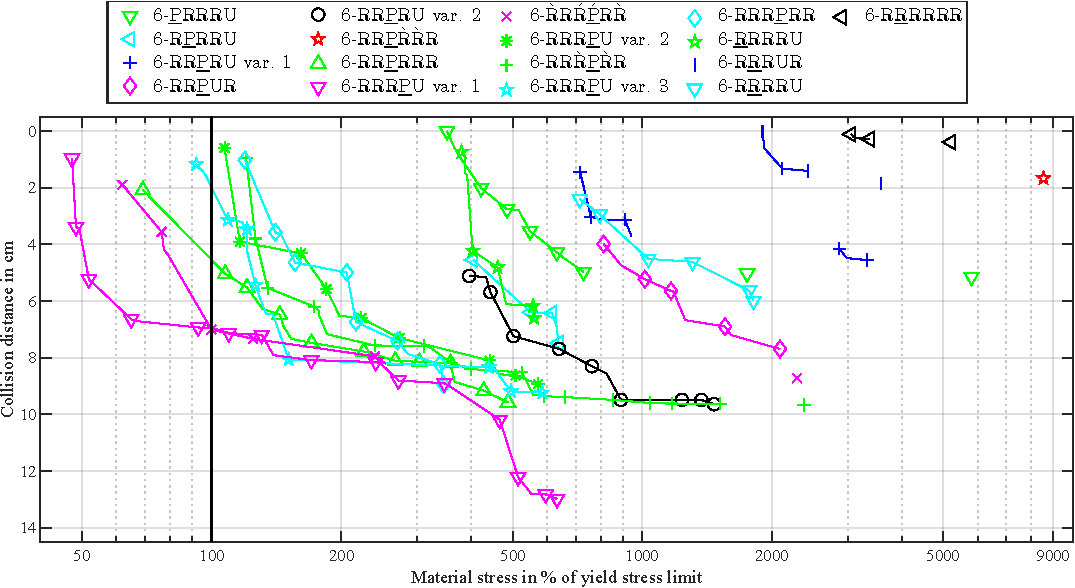
\includegraphics{Figures/lufipkm_pareto_materialstress_colldist_groups_materialstresscolldist_56joints.pdf}
  \end{adjustwidth}
  \caption[Naval-testbed task: \propername{Pareto} fronts for the design-oriented objectives with fixed-dimension lightweight links without link design optimization]{\propername{Pareto} fronts for the design-oriented objectives for chains with five and six joints and fixed-dimension lightweight links without link design optimization.}
  \label{fig:lufipkm_pareto_materialstresscolldist_56joints}
\end{figure}

The \propername{Pareto} diagrams for the drive-train objectives velocity and force are separated into revolute joints in Figure~\ref{fig:lufipkm_pareto_motordiagram_prismatic} and prismatic joints in Figure~\ref{fig:lufipkm_pareto_motordiagram_revolute} since the units are different.
However, the required rated power of 1--2 kW for many structures is similar for both actuation types.
The stronger link dimensioning, visible in Figure~\ref{fig:lufipkm_pareto_linkdiam_colldist}, can partly explain the markers above the ideal hyperbola.
Assumptions regarding transmission ratios (by gear pitch of a spindle or radius of a belt disk), which would allow a unit conversion between rotational and translational quantities, are not included in the synthesis framework.

\vspace{3pt}
\begin{figure}[H]
  \begin{adjustwidth}{-\extralength}{0cm}
    \centering
    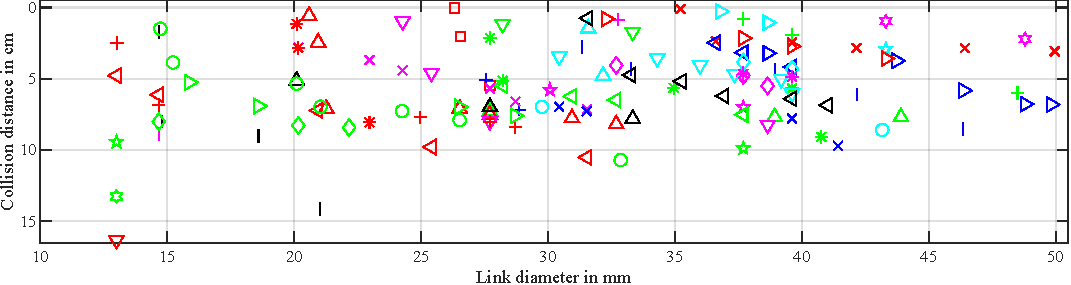
\includegraphics{Figures/lufipkm_pareto_linkdiam_colldist_groups_linkdiam_vs_coll_nolegend.pdf}
  \end{adjustwidth}
  \caption{\propername{Pareto} fronts for the resulting link dimensioning of the results above together with the collision distance as third optimization objective. Only Pareto-dominant particles in these two criteria are shown. The legend is identical to that of Figures~\ref{fig:lufipkm_pareto_motordiagram_prismatic} and~\ref{fig:lufipkm_pareto_motordiagram_revolute}.}
  \label{fig:lufipkm_pareto_linkdiam_colldist}
\end{figure}



\begin{figure}[H]
  \begin{adjustwidth}{-\extralength}{0cm}
    \centering
    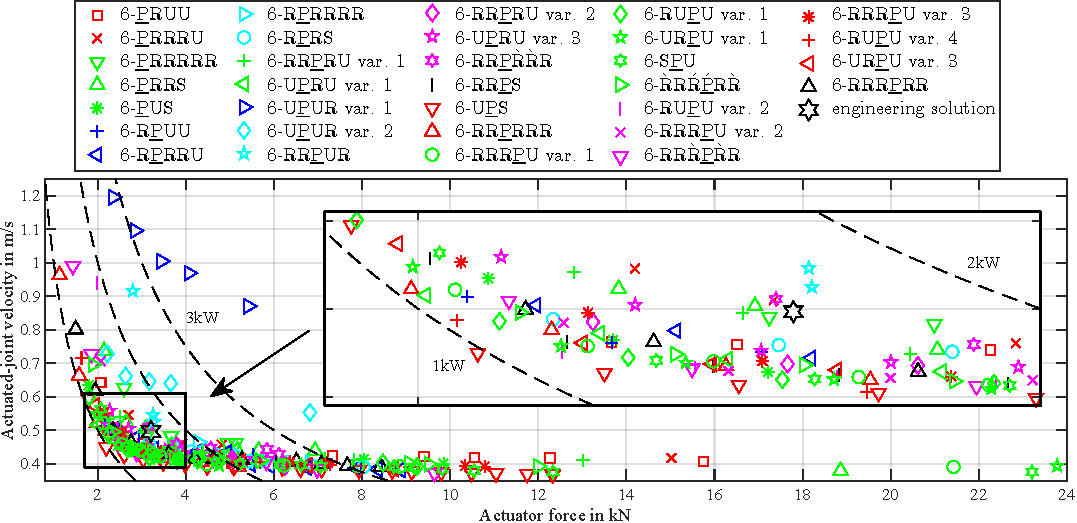
\includegraphics{Figures/lufipkm_pareto_actforce_actvelo_groups_motordiagram_prismatic.pdf}
  \end{adjustwidth}
  \caption{\propername{Pareto} fronts for the actuator-oriented objectives for prismatic actuation.}
  \label{fig:lufipkm_pareto_motordiagram_prismatic}
\end{figure}

\vspace{-6pt}
\begin{figure}[H] 
  \begin{adjustwidth}{-\extralength}{0cm}
    \centering
    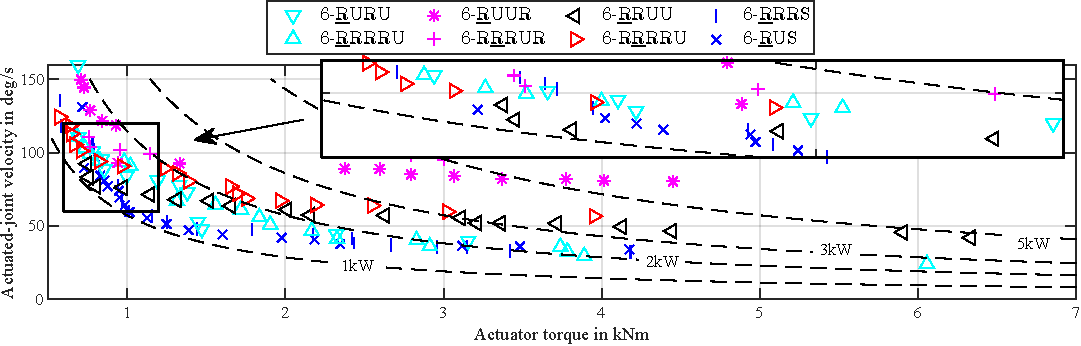
\includegraphics{Figures/lufipkm_pareto_actforce_actvelo_groups_motordiagram_revolute.pdf}
  \end{adjustwidth}
  \caption{\propername{Pareto} fronts for the actuator-oriented objectives for revolute actuation.}
  \label{fig:lufipkm_pareto_motordiagram_revolute}
\end{figure}

\vspace{-6pt}
\begin{figure}[H] 
  \begin{adjustwidth}{-\extralength}{0cm}
    \centering
    \begin{overpic}
      {Figures/lufipkm_compare_GA_vs_PSO.pdf}
      \put(0,0){\textbf{(a)}}
      \put(34,0){\textbf{(b)}}
      \put(67,0){\textbf{(c)}}
    \end{overpic}
  \end{adjustwidth}
  \caption{Comparison of particle swarm optimization (blue) and genetic algorithm (red) for the same settings as Figures~\ref{fig:lufipkm_pareto_motordiagram_prismatic} and~\ref{fig:lufipkm_pareto_motordiagram_revolute} for three different parallel robots (\textbf{a}--\textbf{c}). Each independent repetition has its own marker. The optimal solution after several iterations (from Figures~\ref{fig:lufipkm_pareto_motordiagram_prismatic} and~\ref{fig:lufipkm_pareto_motordiagram_revolute}) is marked in green for reference. Identical markers were thinned out to improve visibility.}
  \label{fig:lufipkm_ga_vs_pso}
\end{figure}



The same drive-train objectives are used for an evaluation of the optimization algorithm.
The synthesis was performed with the multi-objective genetic algorithm and particle swarm optimization with  a random initial population without prior results, set up equally for both.
Default values of the algorithms \cite{Martinez2019,MatlabGOT} were used with 200 individuals and a time limit of eight hours of computation time on the same partition of an Intel Xeon computing cluster \cite{LUISCLUSTER} with \textsc{Matlab} version 2024b.
The experiment was repeated five times with random seeds.
The results are depicted in Figure~\ref{fig:lufipkm_ga_vs_pso} for the 6-U\underline{P}S, 6-\underline{R}US, and 6-\underline{P}US.
The genetic algorithm shows a worse exploration and performance than the PSO, which clearly dominates the GA's results.
For this reason, only the PSO is used within the~paper.


The feasibility of the proposed concept of hierarchical constraints from Section~\ref{sec:ds_optscheme} is evaluated based on the computation times of the single particles of the synthesis above.
All successful parallel robots (187 structures with different chains and coupling-joint alignments) were included with a total of 1.2 %
%
million particles.
A box plot of the computation times over the resulting fitness value (increasing from left to right) is depicted in Figure~\ref{fig:computation_time}.
The fitness values correspond to the constraints from Section~\ref{sec:ds_constraints} that were violated and led to the abortion.
The targeted increasing relation of computation time and validity is evident in the first constraints \ref{itm:constr_param_inclination}--\ref{itm:constr_ik_jac} that account for the plausibility by only checking parameters (\SI{10}{\milli\second} in median) or reference points (up to \SI{5}{\second} in median).
An abortion at the trajectory-related constraints \ref{itm:constr_iktraj}--\ref{itm:constr_jac_traj} (which includes computing all previous constraints) exhibits a required time of 5--20 s.
Reaching the design optimization (constraint~\ref{itm:constr_desopt}) takes about \SI{100}{\second}. The outliers mainly result from structures with many assembly modes (due to multi-joint leg chains) that are all checked.
%
Better handling of this aspect may present a possibility for increasing efficiency in the future.
The evaluation has to be regarded rather qualitatively, as different robots are combined in the box plots, which presents a bias and explains the low median time of the ``success'' case of only \SI{40}{\second}. %

\vspace{-2pt}
\begin{figure}[H]
  \begin{adjustwidth}{-\extralength}{0cm}
    % This file was created by matlab2tikz.
%
%The latest updates can be retrieved from
%  http://www.mathworks.com/matlabcentral/fileexchange/22022-matlab2tikz-matlab2tikz
%where you can also make suggestions and rate matlab2tikz.
%
\begin{tikzpicture}

\begin{axis}[%
width=6.449in,
height=2.52in,
at={(0.496in,0.567in)},
scale only axis,
unbounded coords=jump,
xmin=0,
xmax=28.5,
xtick={1,2,3,4,5,6,7,8,9,10,11,12,13,14,15,16,17,18,19,20,21,22,23,24,25,26,27,28},
xticklabels={{success},{constr. \ref*{itm:constr_desopt}},{constr. \ref*{itm:constr_desopt}},{constr. \ref*{itm:constr_jac_traj}},{constr. \ref*{itm:constr_collinstspc_traj}},{constr. \ref*{itm:constr_collinstspc_traj}},{constr. \ref*{itm:constr_collinstspc_traj}},{constr. \ref*{itm:constr_velo}},{constr. \ref*{itm:constr_velo}},{constr. \ref*{itm:constr_prismaticcylinder_traj}},{constr. \ref*{itm:constr_prismaticcylinder_traj}},{constr. \ref*{itm:constr_jointrange_traj}},{constr. \ref*{itm:constr_jointrange_traj}},{constr. \ref*{itm:constr_iktraj}},{constr. \ref*{itm:constr_workspacecoll}},{constr. \ref*{itm:constr_installspace}},{constr. \ref*{itm:constr_selfcoll}},{constr. \ref*{itm:constr_prismaticcylinder}},{constr. \ref*{itm:constr_prismaticcylinder}},{chainlength},{constr. \ref*{itm:constr_jointrange}},{constr. \ref*{itm:constr_ik_jac}},{constr. \ref*{itm:constr_ik_jac}},{constr. \ref*{itm:constr_ik_succ}},{constr. \ref*{itm:constr_ik_succ}},{constr. \ref*{itm:constr_geom2}},{constr. \ref*{itm:constr_geom1}},{constr. \ref*{itm:constr_param_inclination}--\ref*{itm:constr_param_chainlength}}},
xticklabel style={rotate=90},
ymode=log,
ymin=0.005,
ymax=10000,
ytick={0.01,0.1,1,10,100,1000},
yticklabels={{0.01},{0.1},{1},{10},{100},{1000}},
yminorticks=true,
ylabel style={font=\color{white!15!black}},
ylabel={Time per fitness evaluation in s},
axis background/.style={fill=white},
xmajorgrids,
ymajorgrids,
yminorgrids
]
\addplot [color=black, dashed, forget plot]
  table[row sep=crcr]{%
1	123.786447\\
1	271.074828\\
};
\addplot [color=black, dashed, forget plot]
  table[row sep=crcr]{%
2	154.347325\\
2	277.335092\\
};
\addplot [color=black, dashed, forget plot]
  table[row sep=crcr]{%
3	167.25449875\\
3	313.097785\\
};
\addplot [color=black, dashed, forget plot]
  table[row sep=crcr]{%
4	65.297785\\
4	80.36201\\
};
\addplot [color=black, dashed, forget plot]
  table[row sep=crcr]{%
5	9.09887225\\
5	14.409004\\
};
\addplot [color=black, dashed, forget plot]
  table[row sep=crcr]{%
6	30.01753375\\
6	45.878832\\
};
\addplot [color=black, dashed, forget plot]
  table[row sep=crcr]{%
7	49.234908\\
7	49.234908\\
};
\addplot [color=black, dashed, forget plot]
  table[row sep=crcr]{%
8	6.770948\\
8	8.858536\\
};
\addplot [color=black, dashed, forget plot]
  table[row sep=crcr]{%
9	6.803658\\
9	8.762951\\
};
\addplot [color=black, dashed, forget plot]
  table[row sep=crcr]{%
10	14.341386\\
10	14.641265\\
};
\addplot [color=black, dashed, forget plot]
  table[row sep=crcr]{%
11	7.867104\\
11	7.867104\\
};
\addplot [color=black, dashed, forget plot]
  table[row sep=crcr]{%
12	40.368559\\
12	86.195047\\
};
\addplot [color=black, dashed, forget plot]
  table[row sep=crcr]{%
13	6.8544715\\
13	8.855427\\
};
\addplot [color=black, dashed, forget plot]
  table[row sep=crcr]{%
14	5.93691625\\
14	9.114331\\
};
\addplot [color=black, dashed, forget plot]
  table[row sep=crcr]{%
15	2.925106\\
15	3.681418\\
};
\addplot [color=black, dashed, forget plot]
  table[row sep=crcr]{%
16	6.852222\\
16	13.430652\\
};
\addplot [color=black, dashed, forget plot]
  table[row sep=crcr]{%
17	1.825502\\
17	3.857628\\
};
\addplot [color=black, dashed, forget plot]
  table[row sep=crcr]{%
18	5.5006075\\
18	9.590256\\
};
\addplot [color=black, dashed, forget plot]
  table[row sep=crcr]{%
19	4.4477085\\
19	7.561213\\
};
\addplot [color=black, dashed, forget plot]
  table[row sep=crcr]{%
20	122.180271\\
20	127.62456\\
};
\addplot [color=black, dashed, forget plot]
  table[row sep=crcr]{%
21	3.6166615\\
21	5.330132\\
};
\addplot [color=black, dashed, forget plot]
  table[row sep=crcr]{%
22	4.1684795\\
22	6.895105\\
};
\addplot [color=black, dashed, forget plot]
  table[row sep=crcr]{%
23	4.191057\\
23	4.526031\\
};
\addplot [color=black, dashed, forget plot]
  table[row sep=crcr]{%
24	0.281697\\
24	0.4684\\
};
\addplot [color=black, dashed, forget plot]
  table[row sep=crcr]{%
25	0.1246435\\
25	0.164661\\
};
\addplot [color=black, dashed, forget plot]
  table[row sep=crcr]{%
26	0.075416\\
26	0.107225\\
};
\addplot [color=black, dashed, forget plot]
  table[row sep=crcr]{%
27	0.033777\\
27	0.054247\\
};
\addplot [color=black, dashed, forget plot]
  table[row sep=crcr]{%
28	0.015011\\
28	0.027151\\
};
\addplot [color=black, dashed, forget plot]
  table[row sep=crcr]{%
1	15.102601\\
1	25.592892\\
};
\addplot [color=black, dashed, forget plot]
  table[row sep=crcr]{%
2	27.62244\\
2	71.4961565\\
};
\addplot [color=black, dashed, forget plot]
  table[row sep=crcr]{%
3	37.309894\\
3	68.232941\\
};
\addplot [color=black, dashed, forget plot]
  table[row sep=crcr]{%
4	25.053854\\
4	31.7947105\\
};
\addplot [color=black, dashed, forget plot]
  table[row sep=crcr]{%
5	3.643429\\
5	5.47933925\\
};
\addplot [color=black, dashed, forget plot]
  table[row sep=crcr]{%
6	9.210458\\
6	14.608325\\
};
\addplot [color=black, dashed, forget plot]
  table[row sep=crcr]{%
7	15.935245\\
7	18.065945\\
};
\addplot [color=black, dashed, forget plot]
  table[row sep=crcr]{%
8	4.527528\\
8	5.347809\\
};
\addplot [color=black, dashed, forget plot]
  table[row sep=crcr]{%
9	4.324491\\
9	5.409103\\
};
\addplot [color=black, dashed, forget plot]
  table[row sep=crcr]{%
10	4.915937\\
10	7.26997625\\
};
\addplot [color=black, dashed, forget plot]
  table[row sep=crcr]{%
11	7.867104\\
11	7.867104\\
};
\addplot [color=black, dashed, forget plot]
  table[row sep=crcr]{%
12	5.508612\\
12	8.859749\\
};
\addplot [color=black, dashed, forget plot]
  table[row sep=crcr]{%
13	4.627161\\
13	5.4296965\\
};
\addplot [color=black, dashed, forget plot]
  table[row sep=crcr]{%
14	2.845271\\
14	3.69286825\\
};
\addplot [color=black, dashed, forget plot]
  table[row sep=crcr]{%
15	1.707995\\
15	2.2772075\\
};
\addplot [color=black, dashed, forget plot]
  table[row sep=crcr]{%
16	1.270619\\
16	2.4665\\
};
\addplot [color=black, dashed, forget plot]
  table[row sep=crcr]{%
17	0.106743\\
17	0.4707\\
};
\addplot [color=black, dashed, forget plot]
  table[row sep=crcr]{%
18	1.463367\\
18	2.65742525\\
};
\addplot [color=black, dashed, forget plot]
  table[row sep=crcr]{%
19	1.660119\\
19	2.3507675\\
};
\addplot [color=black, dashed, forget plot]
  table[row sep=crcr]{%
20	57.058059\\
20	80.1052335\\
};
\addplot [color=black, dashed, forget plot]
  table[row sep=crcr]{%
21	1.410055\\
21	2.4693495\\
};
\addplot [color=black, dashed, forget plot]
  table[row sep=crcr]{%
22	1.065499\\
22	2.349917\\
};
\addplot [color=black, dashed, forget plot]
  table[row sep=crcr]{%
23	1.575555\\
23	1.927044\\
};
\addplot [color=black, dashed, forget plot]
  table[row sep=crcr]{%
24	0.085762\\
24	0.157222\\
};
\addplot [color=black, dashed, forget plot]
  table[row sep=crcr]{%
25	0.08368\\
25	0.097934\\
};
\addplot [color=black, dashed, forget plot]
  table[row sep=crcr]{%
26	0.037148\\
26	0.054207\\
};
\addplot [color=black, dashed, forget plot]
  table[row sep=crcr]{%
27	0.008005\\
27	0.020129\\
};
\addplot [color=black, dashed, forget plot]
  table[row sep=crcr]{%
28	0.002149\\
28	0.006917\\
};
\addplot [color=black, forget plot]
  table[row sep=crcr]{%
0.875	271.074828\\
1.125	271.074828\\
};
\addplot [color=black, forget plot]
  table[row sep=crcr]{%
1.875	277.335092\\
2.125	277.335092\\
};
\addplot [color=black, forget plot]
  table[row sep=crcr]{%
2.875	313.097785\\
3.125	313.097785\\
};
\addplot [color=black, forget plot]
  table[row sep=crcr]{%
3.875	80.36201\\
4.125	80.36201\\
};
\addplot [color=black, forget plot]
  table[row sep=crcr]{%
4.875	14.409004\\
5.125	14.409004\\
};
\addplot [color=black, forget plot]
  table[row sep=crcr]{%
5.875	45.878832\\
6.125	45.878832\\
};
\addplot [color=black, forget plot]
  table[row sep=crcr]{%
6.875	49.234908\\
7.125	49.234908\\
};
\addplot [color=black, forget plot]
  table[row sep=crcr]{%
7.875	8.858536\\
8.125	8.858536\\
};
\addplot [color=black, forget plot]
  table[row sep=crcr]{%
8.875	8.762951\\
9.125	8.762951\\
};
\addplot [color=black, forget plot]
  table[row sep=crcr]{%
9.875	14.641265\\
10.125	14.641265\\
};
\addplot [color=black, forget plot]
  table[row sep=crcr]{%
10.875	7.867104\\
11.125	7.867104\\
};
\addplot [color=black, forget plot]
  table[row sep=crcr]{%
11.875	86.195047\\
12.125	86.195047\\
};
\addplot [color=black, forget plot]
  table[row sep=crcr]{%
12.875	8.855427\\
13.125	8.855427\\
};
\addplot [color=black, forget plot]
  table[row sep=crcr]{%
13.875	9.114331\\
14.125	9.114331\\
};
\addplot [color=black, forget plot]
  table[row sep=crcr]{%
14.875	3.681418\\
15.125	3.681418\\
};
\addplot [color=black, forget plot]
  table[row sep=crcr]{%
15.875	13.430652\\
16.125	13.430652\\
};
\addplot [color=black, forget plot]
  table[row sep=crcr]{%
16.875	3.857628\\
17.125	3.857628\\
};
\addplot [color=black, forget plot]
  table[row sep=crcr]{%
17.875	9.590256\\
18.125	9.590256\\
};
\addplot [color=black, forget plot]
  table[row sep=crcr]{%
18.875	7.561213\\
19.125	7.561213\\
};
\addplot [color=black, forget plot]
  table[row sep=crcr]{%
19.875	127.62456\\
20.125	127.62456\\
};
\addplot [color=black, forget plot]
  table[row sep=crcr]{%
20.875	5.330132\\
21.125	5.330132\\
};
\addplot [color=black, forget plot]
  table[row sep=crcr]{%
21.875	6.895105\\
22.125	6.895105\\
};
\addplot [color=black, forget plot]
  table[row sep=crcr]{%
22.875	4.526031\\
23.125	4.526031\\
};
\addplot [color=black, forget plot]
  table[row sep=crcr]{%
23.875	0.4684\\
24.125	0.4684\\
};
\addplot [color=black, forget plot]
  table[row sep=crcr]{%
24.875	0.164661\\
25.125	0.164661\\
};
\addplot [color=black, forget plot]
  table[row sep=crcr]{%
25.875	0.107225\\
26.125	0.107225\\
};
\addplot [color=black, forget plot]
  table[row sep=crcr]{%
26.875	0.054247\\
27.125	0.054247\\
};
\addplot [color=black, forget plot]
  table[row sep=crcr]{%
27.875	0.027151\\
28.125	0.027151\\
};
\addplot [color=black, forget plot]
  table[row sep=crcr]{%
0.875	15.102601\\
1.125	15.102601\\
};
\addplot [color=black, forget plot]
  table[row sep=crcr]{%
1.875	27.62244\\
2.125	27.62244\\
};
\addplot [color=black, forget plot]
  table[row sep=crcr]{%
2.875	37.309894\\
3.125	37.309894\\
};
\addplot [color=black, forget plot]
  table[row sep=crcr]{%
3.875	25.053854\\
4.125	25.053854\\
};
\addplot [color=black, forget plot]
  table[row sep=crcr]{%
4.875	3.643429\\
5.125	3.643429\\
};
\addplot [color=black, forget plot]
  table[row sep=crcr]{%
5.875	9.210458\\
6.125	9.210458\\
};
\addplot [color=black, forget plot]
  table[row sep=crcr]{%
6.875	15.935245\\
7.125	15.935245\\
};
\addplot [color=black, forget plot]
  table[row sep=crcr]{%
7.875	4.527528\\
8.125	4.527528\\
};
\addplot [color=black, forget plot]
  table[row sep=crcr]{%
8.875	4.324491\\
9.125	4.324491\\
};
\addplot [color=black, forget plot]
  table[row sep=crcr]{%
9.875	4.915937\\
10.125	4.915937\\
};
\addplot [color=black, forget plot]
  table[row sep=crcr]{%
10.875	7.867104\\
11.125	7.867104\\
};
\addplot [color=black, forget plot]
  table[row sep=crcr]{%
11.875	5.508612\\
12.125	5.508612\\
};
\addplot [color=black, forget plot]
  table[row sep=crcr]{%
12.875	4.627161\\
13.125	4.627161\\
};
\addplot [color=black, forget plot]
  table[row sep=crcr]{%
13.875	2.845271\\
14.125	2.845271\\
};
\addplot [color=black, forget plot]
  table[row sep=crcr]{%
14.875	1.707995\\
15.125	1.707995\\
};
\addplot [color=black, forget plot]
  table[row sep=crcr]{%
15.875	1.270619\\
16.125	1.270619\\
};
\addplot [color=black, forget plot]
  table[row sep=crcr]{%
16.875	0.106743\\
17.125	0.106743\\
};
\addplot [color=black, forget plot]
  table[row sep=crcr]{%
17.875	1.463367\\
18.125	1.463367\\
};
\addplot [color=black, forget plot]
  table[row sep=crcr]{%
18.875	1.660119\\
19.125	1.660119\\
};
\addplot [color=black, forget plot]
  table[row sep=crcr]{%
19.875	57.058059\\
20.125	57.058059\\
};
\addplot [color=black, forget plot]
  table[row sep=crcr]{%
20.875	1.410055\\
21.125	1.410055\\
};
\addplot [color=black, forget plot]
  table[row sep=crcr]{%
21.875	1.065499\\
22.125	1.065499\\
};
\addplot [color=black, forget plot]
  table[row sep=crcr]{%
22.875	1.575555\\
23.125	1.575555\\
};
\addplot [color=black, forget plot]
  table[row sep=crcr]{%
23.875	0.085762\\
24.125	0.085762\\
};
\addplot [color=black, forget plot]
  table[row sep=crcr]{%
24.875	0.08368\\
25.125	0.08368\\
};
\addplot [color=black, forget plot]
  table[row sep=crcr]{%
25.875	0.037148\\
26.125	0.037148\\
};
\addplot [color=black, forget plot]
  table[row sep=crcr]{%
26.875	0.008005\\
27.125	0.008005\\
};
\addplot [color=black, forget plot]
  table[row sep=crcr]{%
27.875	0.002149\\
28.125	0.002149\\
};
\addplot [color=blue, forget plot]
  table[row sep=crcr]{%
0.75	25.592892\\
0.75	123.786447\\
1.25	123.786447\\
1.25	25.592892\\
0.75	25.592892\\
};
\addplot [color=blue, forget plot]
  table[row sep=crcr]{%
1.75	71.4961565\\
1.75	154.347325\\
2.25	154.347325\\
2.25	71.4961565\\
1.75	71.4961565\\
};
\addplot [color=blue, forget plot]
  table[row sep=crcr]{%
2.75	68.232941\\
2.75	167.25449875\\
3.25	167.25449875\\
3.25	68.232941\\
2.75	68.232941\\
};
\addplot [color=blue, forget plot]
  table[row sep=crcr]{%
3.75	31.7947105\\
3.75	65.297785\\
4.25	65.297785\\
4.25	31.7947105\\
3.75	31.7947105\\
};
\addplot [color=blue, forget plot]
  table[row sep=crcr]{%
4.75	5.47933925\\
4.75	9.09887225\\
5.25	9.09887225\\
5.25	5.47933925\\
4.75	5.47933925\\
};
\addplot [color=blue, forget plot]
  table[row sep=crcr]{%
5.75	14.608325\\
5.75	30.01753375\\
6.25	30.01753375\\
6.25	14.608325\\
5.75	14.608325\\
};
\addplot [color=blue, forget plot]
  table[row sep=crcr]{%
6.75	18.065945\\
6.75	49.234908\\
7.25	49.234908\\
7.25	18.065945\\
6.75	18.065945\\
};
\addplot [color=blue, forget plot]
  table[row sep=crcr]{%
7.75	5.347809\\
7.75	6.770948\\
8.25	6.770948\\
8.25	5.347809\\
7.75	5.347809\\
};
\addplot [color=blue, forget plot]
  table[row sep=crcr]{%
8.75	5.409103\\
8.75	6.803658\\
9.25	6.803658\\
9.25	5.409103\\
8.75	5.409103\\
};
\addplot [color=blue, forget plot]
  table[row sep=crcr]{%
9.75	7.26997625\\
9.75	14.341386\\
10.25	14.341386\\
10.25	7.26997625\\
9.75	7.26997625\\
};
\addplot [color=blue, forget plot]
  table[row sep=crcr]{%
10.75	7.867104\\
10.75	7.867104\\
11.25	7.867104\\
11.25	7.867104\\
10.75	7.867104\\
};
\addplot [color=blue, forget plot]
  table[row sep=crcr]{%
11.75	8.859749\\
11.75	40.368559\\
12.25	40.368559\\
12.25	8.859749\\
11.75	8.859749\\
};
\addplot [color=blue, forget plot]
  table[row sep=crcr]{%
12.75	5.4296965\\
12.75	6.8544715\\
13.25	6.8544715\\
13.25	5.4296965\\
12.75	5.4296965\\
};
\addplot [color=blue, forget plot]
  table[row sep=crcr]{%
13.75	3.69286825\\
13.75	5.93691625\\
14.25	5.93691625\\
14.25	3.69286825\\
13.75	3.69286825\\
};
\addplot [color=blue, forget plot]
  table[row sep=crcr]{%
14.75	2.2772075\\
14.75	2.925106\\
15.25	2.925106\\
15.25	2.2772075\\
14.75	2.2772075\\
};
\addplot [color=blue, forget plot]
  table[row sep=crcr]{%
15.75	2.4665\\
15.75	6.852222\\
16.25	6.852222\\
16.25	2.4665\\
15.75	2.4665\\
};
\addplot [color=blue, forget plot]
  table[row sep=crcr]{%
16.75	0.4707\\
16.75	1.825502\\
17.25	1.825502\\
17.25	0.4707\\
16.75	0.4707\\
};
\addplot [color=blue, forget plot]
  table[row sep=crcr]{%
17.75	2.65742525\\
17.75	5.5006075\\
18.25	5.5006075\\
18.25	2.65742525\\
17.75	2.65742525\\
};
\addplot [color=blue, forget plot]
  table[row sep=crcr]{%
18.75	2.3507675\\
18.75	4.4477085\\
19.25	4.4477085\\
19.25	2.3507675\\
18.75	2.3507675\\
};
\addplot [color=blue, forget plot]
  table[row sep=crcr]{%
19.75	80.1052335\\
19.75	122.180271\\
20.25	122.180271\\
20.25	80.1052335\\
19.75	80.1052335\\
};
\addplot [color=blue, forget plot]
  table[row sep=crcr]{%
20.75	2.4693495\\
20.75	3.6166615\\
21.25	3.6166615\\
21.25	2.4693495\\
20.75	2.4693495\\
};
\addplot [color=blue, forget plot]
  table[row sep=crcr]{%
21.75	2.349917\\
21.75	4.1684795\\
22.25	4.1684795\\
22.25	2.349917\\
21.75	2.349917\\
};
\addplot [color=blue, forget plot]
  table[row sep=crcr]{%
22.75	1.927044\\
22.75	4.191057\\
23.25	4.191057\\
23.25	1.927044\\
22.75	1.927044\\
};
\addplot [color=blue, forget plot]
  table[row sep=crcr]{%
23.75	0.157222\\
23.75	0.281697\\
24.25	0.281697\\
24.25	0.157222\\
23.75	0.157222\\
};
\addplot [color=blue, forget plot]
  table[row sep=crcr]{%
24.75	0.097934\\
24.75	0.1246435\\
25.25	0.1246435\\
25.25	0.097934\\
24.75	0.097934\\
};
\addplot [color=blue, forget plot]
  table[row sep=crcr]{%
25.75	0.054207\\
25.75	0.075416\\
26.25	0.075416\\
26.25	0.054207\\
25.75	0.054207\\
};
\addplot [color=blue, forget plot]
  table[row sep=crcr]{%
26.75	0.020129\\
26.75	0.033777\\
27.25	0.033777\\
27.25	0.020129\\
26.75	0.020129\\
};
\addplot [color=blue, forget plot]
  table[row sep=crcr]{%
27.75	0.006917\\
27.75	0.015011\\
28.25	0.015011\\
28.25	0.006917\\
27.75	0.006917\\
};
\addplot [color=red, forget plot]
  table[row sep=crcr]{%
0.75	34.1471385\\
1.25	34.1471385\\
};
\addplot [color=red, forget plot]
  table[row sep=crcr]{%
1.75	107.984888\\
2.25	107.984888\\
};
\addplot [color=red, forget plot]
  table[row sep=crcr]{%
2.75	112.519567\\
3.25	112.519567\\
};
\addplot [color=red, forget plot]
  table[row sep=crcr]{%
3.75	42.9711515\\
4.25	42.9711515\\
};
\addplot [color=red, forget plot]
  table[row sep=crcr]{%
4.75	8.268415\\
5.25	8.268415\\
};
\addplot [color=red, forget plot]
  table[row sep=crcr]{%
5.75	19.827957\\
6.25	19.827957\\
};
\addplot [color=red, forget plot]
  table[row sep=crcr]{%
6.75	31.3085815\\
7.25	31.3085815\\
};
\addplot [color=red, forget plot]
  table[row sep=crcr]{%
7.75	6.042387\\
8.25	6.042387\\
};
\addplot [color=red, forget plot]
  table[row sep=crcr]{%
8.75	6.0866835\\
9.25	6.0866835\\
};
\addplot [color=red, forget plot]
  table[row sep=crcr]{%
9.75	11.190725\\
10.25	11.190725\\
};
\addplot [color=red, forget plot]
  table[row sep=crcr]{%
10.75	7.867104\\
11.25	7.867104\\
};
\addplot [color=red, forget plot]
  table[row sep=crcr]{%
11.75	19.7779065\\
12.25	19.7779065\\
};
\addplot [color=red, forget plot]
  table[row sep=crcr]{%
12.75	6.113933\\
13.25	6.113933\\
};
\addplot [color=red, forget plot]
  table[row sep=crcr]{%
13.75	4.525064\\
14.25	4.525064\\
};
\addplot [color=red, forget plot]
  table[row sep=crcr]{%
14.75	2.554502\\
15.25	2.554502\\
};
\addplot [color=red, forget plot]
  table[row sep=crcr]{%
15.75	3.527561\\
16.25	3.527561\\
};
\addplot [color=red, forget plot]
  table[row sep=crcr]{%
16.75	0.816999\\
17.25	0.816999\\
};
\addplot [color=red, forget plot]
  table[row sep=crcr]{%
17.75	3.266164\\
18.25	3.266164\\
};
\addplot [color=red, forget plot]
  table[row sep=crcr]{%
18.75	2.895795\\
19.25	2.895795\\
};
\addplot [color=red, forget plot]
  table[row sep=crcr]{%
19.75	97.003035\\
20.25	97.003035\\
};
\addplot [color=red, forget plot]
  table[row sep=crcr]{%
20.75	2.912858\\
21.25	2.912858\\
};
\addplot [color=red, forget plot]
  table[row sep=crcr]{%
21.75	2.8717145\\
22.25	2.8717145\\
};
\addplot [color=red, forget plot]
  table[row sep=crcr]{%
22.75	2.322527\\
23.25	2.322527\\
};
\addplot [color=red, forget plot]
  table[row sep=crcr]{%
23.75	0.206886\\
24.25	0.206886\\
};
\addplot [color=red, forget plot]
  table[row sep=crcr]{%
24.75	0.10675\\
25.25	0.10675\\
};
\addplot [color=red, forget plot]
  table[row sep=crcr]{%
25.75	0.0630445\\
26.25	0.0630445\\
};
\addplot [color=red, forget plot]
  table[row sep=crcr]{%
26.75	0.025934\\
27.25	0.025934\\
};
\addplot [color=red, forget plot]
  table[row sep=crcr]{%
27.75	0.010296\\
28.25	0.010296\\
};
\addplot [color=black, only marks, mark=+, mark options={solid, draw=red}, forget plot]
  table[row sep=crcr]{%
1	271.078109\\
1	352.421981\\
1	458.30276\\
1	595.939549\\
1	776.998656\\
1	1010.709355\\
1	1328.666596\\
1	1730.959515\\
1	2264.6653\\
1	3117.685149\\
1	5196.786853\\
1	9146.318036\\
};
\addplot [color=black, only marks, mark=+, mark options={solid, draw=red}, forget plot]
  table[row sep=crcr]{%
2	279.856683\\
2	366.752712\\
2	477.112975\\
2	628.909301\\
2	831.798361\\
2	1349.86609\\
2	1375.419227\\
};
\addplot [color=black, only marks, mark=+, mark options={solid, draw=red}, forget plot]
  table[row sep=crcr]{%
3	318.405353\\
3	415.310058\\
3	542.668544\\
3	708.086027\\
3	948.18956\\
3	1305.810499\\
3	2048.918539\\
};
\addplot [color=black, only marks, mark=+, mark options={solid, draw=red}, forget plot]
  table[row sep=crcr]{%
4	234.919049\\
4	308.154177\\
4	320.272458\\
};
\addplot [color=black, only marks, mark=+, mark options={solid, draw=red}, forget plot]
  table[row sep=crcr]{%
5	14.545025\\
5	19.057092\\
5	25.203607\\
5	46.378056\\
5	77.318439\\
5	169.613583\\
};
\addplot [color=black, only marks, mark=+, mark options={solid, draw=red}, forget plot]
  table[row sep=crcr]{%
6	53.930537\\
6	82.461856\\
};
\addplot [color=black, only marks, mark=+, mark options={solid, draw=red}, forget plot]
  table[row sep=crcr]{%
7	298.699656\\
};
\addplot [color=black, only marks, mark=+, mark options={solid, draw=red}, forget plot]
  table[row sep=crcr]{%
8	9.135066\\
8	11.994717\\
8	22.567487\\
8	32.026793\\
8	44.400364\\
8	70.678086\\
8	92.19582\\
8	121.146369\\
8	146.904329\\
};
\addplot [color=black, only marks, mark=+, mark options={solid, draw=red}, forget plot]
  table[row sep=crcr]{%
9	8.956132\\
9	13.480079\\
9	90.711184\\
9	93.681337\\
};
\addplot [color=black, only marks, mark=+, mark options={solid, draw=red}, forget plot]
  table[row sep=crcr]{%
10	43.927161\\
10	70.267663\\
};
\addplot [color=black, only marks, mark=+, mark options={solid, draw=red}, forget plot]
  table[row sep=crcr]{%
nan	nan\\
};
\addplot [color=black, only marks, mark=+, mark options={solid, draw=red}, forget plot]
  table[row sep=crcr]{%
12	88.368955\\
12	134.620493\\
};
\addplot [color=black, only marks, mark=+, mark options={solid, draw=red}, forget plot]
  table[row sep=crcr]{%
13	9.085692\\
13	13.019501\\
13	36.601829\\
13	84.074043\\
13	93.947386\\
};
\addplot [color=black, only marks, mark=+, mark options={solid, draw=red}, forget plot]
  table[row sep=crcr]{%
14	14.933917\\
14	19.421108\\
14	27.621206\\
14	30.272053\\
};
\addplot [color=black, only marks, mark=+, mark options={solid, draw=red}, forget plot]
  table[row sep=crcr]{%
15	4.098754\\
15	6.152144\\
15	8.308653\\
15	31.516832\\
15	46.073932\\
};
\addplot [color=black, only marks, mark=+, mark options={solid, draw=red}, forget plot]
  table[row sep=crcr]{%
16	13.431123\\
16	17.463061\\
16	22.704365\\
16	29.516442\\
16	38.374283\\
16	49.898962\\
16	64.874384\\
16	84.354762\\
16	109.723298\\
16	142.734211\\
16	185.884174\\
16	250.803122\\
};
\addplot [color=black, only marks, mark=+, mark options={solid, draw=red}, forget plot]
  table[row sep=crcr]{%
17	3.857736\\
17	5.015174\\
17	6.519734\\
17	8.47613\\
17	11.020519\\
17	14.327557\\
17	18.626842\\
17	24.220807\\
17	31.501566\\
17	40.955365\\
17	53.242779\\
17	69.27933\\
17	90.091647\\
17	119.780563\\
17	158.491096\\
17	162.379267\\
};
\addplot [color=black, only marks, mark=+, mark options={solid, draw=red}, forget plot]
  table[row sep=crcr]{%
18	11.3422\\
18	62.411237\\
18	81.52526\\
18	85.853589\\
};
\addplot [color=black, only marks, mark=+, mark options={solid, draw=red}, forget plot]
  table[row sep=crcr]{%
19	7.782762\\
19	53.521119\\
19	78.227987\\
19	92.192788\\
};
\addplot [color=black, only marks, mark=+, mark options={solid, draw=red}, forget plot]
  table[row sep=crcr]{%
20	187.381133\\
20	198.370046\\
};
\addplot [color=black, only marks, mark=+, mark options={solid, draw=red}, forget plot]
  table[row sep=crcr]{%
21	5.345269\\
21	6.95057\\
21	9.03665\\
21	12.856193\\
21	17.753034\\
21	23.229282\\
21	30.336197\\
21	40.851434\\
21	53.272551\\
21	69.288468\\
21	90.266323\\
21	122.874625\\
21	169.927749\\
21	218.528757\\
};
\addplot [color=black, only marks, mark=+, mark options={solid, draw=red}, forget plot]
  table[row sep=crcr]{%
22	6.896658\\
22	8.965898\\
22	11.661467\\
22	16.299648\\
22	21.287851\\
22	29.538094\\
22	43.203421\\
22	57.41653\\
22	75.063658\\
22	97.677503\\
22	130.622795\\
22	173.732205\\
22	193.319214\\
};
\addplot [color=black, only marks, mark=+, mark options={solid, draw=red}, forget plot]
  table[row sep=crcr]{%
23	8.799476\\
};
\addplot [color=black, only marks, mark=+, mark options={solid, draw=red}, forget plot]
  table[row sep=crcr]{%
24	0.46841\\
24	0.60899\\
24	0.791759\\
24	1.029318\\
24	1.338206\\
24	1.740593\\
24	2.263252\\
24	2.951134\\
24	3.886721\\
24	5.110682\\
24	6.675241\\
24	10.61063\\
};
\addplot [color=black, only marks, mark=+, mark options={solid, draw=red}, forget plot]
  table[row sep=crcr]{%
25	0.164744\\
25	0.215319\\
25	0.28247\\
25	0.370143\\
25	0.487234\\
25	0.643632\\
};
\addplot [color=black, only marks, mark=+, mark options={solid, draw=red}, forget plot]
  table[row sep=crcr]{%
26	0.107234\\
26	0.139409\\
26	0.18125\\
26	0.235677\\
26	0.306838\\
26	0.399505\\
26	0.519692\\
26	0.688134\\
26	0.939355\\
26	1.221615\\
26	1.420865\\
};
\addplot [color=black, only marks, mark=+, mark options={solid, draw=red}, forget plot]
  table[row sep=crcr]{%
27	0.054258\\
27	0.070561\\
27	0.091737\\
27	0.11953\\
27	0.156528\\
27	0.206944\\
27	0.270097\\
27	0.35309\\
27	0.480275\\
27	0.627522\\
27	0.844434\\
};
\addplot [color=black, only marks, mark=+, mark options={solid, draw=red}, forget plot]
  table[row sep=crcr]{%
28	0.027153\\
28	0.035299\\
28	0.045891\\
28	0.059664\\
28	0.077702\\
28	0.101094\\
28	0.131586\\
28	0.171292\\
28	0.222751\\
28	0.290282\\
28	0.37888\\
28	0.496756\\
28	0.64963\\
28	0.871419\\
28	1.190338\\
28	1.623173\\
28	1.835289\\
};
\end{axis}

\begin{axis}[%
width=7.087in,
height=3.15in,
at={(0in,0in)},
scale only axis,
xmin=0,
xmax=1,
ymin=0,
ymax=1,
axis line style={draw=none},
ticks=none,
axis x line*=bottom,
axis y line*=left
]
\end{axis}
\end{tikzpicture}%
  \end{adjustwidth}
  \caption{Computation
    time of the fitness function (logarithmic scale) in relation to the number of the violated constraint (from Section~\ref{sec:ds_constraints}) that led to abortion. The class ``chainlength'' comes from checking if the length of a leg chain that includes a prismatic joint exceeds the maximum allowed length. Outlier markers were thinned out (193 of 97 k left over) to increase visibility of the data. Duplicate constraints result from multiple similar checks, e.g., for different Jacobian matrices in constraint~\ref*{itm:constr_ik_jac}.}
  \label{fig:computation_time}
\end{figure}


One parameterization is chosen for each of the valid parallel robots from the \propername{Pareto} diagrams.
The selection is based on the \propername{Pareto} diagram of collision distance vs. actuator power in Figure~\ref{fig:lufipkm_pareto_power_mass_groups}. 
Both criteria are normalized to their best-achieved values (for all structures), and the best particle for equal weighting is chosen to illustrate the results' appearance.
The performance values and kinematic parameters of these reference solutions are summarized in Table~\ref{tab:lufipkm_results_pris} for prismatic and Table~\ref{tab:lufipkm_results_rev} for revolute actuation.
Kinematic sketches are given in Figures~\ref{fig:lufipkm_robots2}--\ref{fig:lufipkm_robots4}.

\begin{table}[H]
  \caption{Summary
    of one typical particle for each robot with \emph{prismatic actuation}, visualized in Figures~\ref{fig:lufipkm_robots2} and \ref{fig:lufipkm_robots3}. Abbreviations: ``coll.'' (collision distance), ``velo.'' (actuator velocity), ``cond.'' (largest \propername{Jacobian} condition number), $n$ (number of optimization variables), $r_\mathrm{b}$ (base radius), $d_\mathrm{b}$ (base-joint pair distance), $\gamma_\mathrm{b}$ (base-joint inclination), $r_\mathrm{p}$ (platform radius), $d_\mathrm{p}$ (platform-joint pair distance), $e_\mathrm{link}$ (material strength of the links), $d_\mathrm{link}$ (diameter of the links), ``Eng. Sol.'' engineering solution. Continued horizontally in Table~\ref{tab:lufipkm_results_pris_dh}.}
  \begin{adjustwidth}{-\extralength}{0cm}
    \centering
    \label{tab:lufipkm_results_pris}
    \begin{tabularx}{\fulllength}{lRRRRRRRRRRRRR} %
      \toprule
      \multicolumn{1}{c}{\textbf{Robot}}
      & \multicolumn{5}{c}{\textbf{Performance}} & \multicolumn{8}{c}{\textbf{Kinematic and Design Parameters}} \\
      \midrule
      & \multicolumn{1}{r}{coll.} & \multicolumn{1}{r}{power} & \multicolumn{1}{r}{force} & \multicolumn{1}{r}{velo.} & \multicolumn{1}{r}{cond.} &  \multicolumn{1}{c}{$n$} &
      \multicolumn{1}{c}{$r_\mathrm{b}$} & \multicolumn{1}{c}{$d_\mathrm{b}$} & \multicolumn{1}{c}{$\gamma_\mathrm{b}$} & \multicolumn{1}{c}{$r_\mathrm{p}$}& \multicolumn{1}{c}{$d_\mathrm{p}$} & \multicolumn{1}{c}{$e_\mathrm{link}$} & \multicolumn{1}{c}{$d_\mathrm{link}$} \\
      & \multicolumn{1}{c}{mm} & \multicolumn{1}{c}{kW} & \multicolumn{1}{c}{kN} & \multicolumn{1}{c}{m/s} & \multicolumn{1}{c}{} & & \multicolumn{1}{c}{mm} & \multicolumn{1}{c}{mm} & \multicolumn{1}{c}{deg} & \multicolumn{1}{c}{mm} & \multicolumn{1}{c}{mm} & \multicolumn{1}{c}{mm} & \multicolumn{1}{c}{mm} \\
      \midrule %
      \hyperrefl{restabrow:P6PRRRRR4V2GxPxA1}{6-\underline{P}{R}{U}{U}},\,C-R & 18 & 1.15 & 2.17 & 0.53 & 25 & 16 & 613 & 219 & 37 & 165 & 346 & 11 & 27 \\ % group 1; lufipkm_20230413_Diss_processworkspace_allrob_default/Rob454_P6PRRRRR4V2G8P6A1 (Pareto-Index 1)
\hyperrefl{restabrow:P6PRRRRR4V3GxPxA1}{6-\underline{P}{R}{R}{R}{U}},\,V-R & 0 & 1.45 & 2.73 & 0.53 & 24 & 17 & 495 & 618 & 0 & 212 & 219 & 10 & 40 \\ % group 2; lufipkm_20230418_Diss_processworkspace_robotsfrom0415_default2/Rob21_P6PRRRRR4V3G5P6A1 (Pareto-Index 1)
\midrule
\hyperrefl{restabrow:P6PRRRRR6GxPxA1}{6-\underline{P}{R}{R}{R}{R}{R}},\,C-T & 10 & 1.82 & 3.47 & 0.52 & 50 & 21 & 410 & 255 & 173 & 152 & 275 & 14 & 31 \\ % group 3; lufipkm_20230418_Diss_processworkspace_robotsfrom0415_default2/Rob23_P6PRRRRR6G8P5A1 (Pareto-Index 1)
\hyperrefl{restabrow:P6PRRRRR6V2GxPxA1}{6-\underline{P}{R}{R}{S}},\,V-V & 69 & 1.62 & 2.89 & 0.56 & 23 & 16 & 551 & 254 & 0 & 194 & 273 & 10 & 36 \\ % group 4; lufipkm_20230413_Diss_processworkspace_allrob_default/Rob686_P6PRRRRR6V2G5P4A1 (Pareto-Index 3)
\hyperrefl{restabrow:P6PRRRRR6V4GxPxA1}{6-\underline{P}{U}{S}},\,V-V & 35 & 1.28 & 2.46 & 0.52 & 23 & 13 & 534 & 257 & 0 & 174 & 320 & 4 & 33 \\ % group 5; lufipkm_20230413_Diss_processworkspace_allrob_default/Rob706_P6PRRRRR6V4G5P4A1 (Pareto-Index 5)
\midrule
\hyperrefl{restabrow:P6RPRRRR10V5GxPxA2}{6-{R}\underline{P}{U}{U}},\,R-R & 69 & 1.42 & 3.03 & 0.47 & 25 & 13 & 722 & 159 & 0 & 183 & 287 & 12 & 32 \\ % group 6; lufipkm_20230413_Diss_processworkspace_allrob_default/Rob840_P6RPRRRR10V5G7P6A1 (Pareto-Index 9)
\hyperrefl{restabrow:P6RPRRRR10V6GxPxA2}{6-{R}\underline{P}{R}{R}{U}},\,C-R & 14 & 1.94 & 4.06 & 0.48 & 30 & 16 & 536 & 269 & 33 & 210 & 233 & 10 & 37 \\ % group 7; lufipkm_20230418_Diss_processworkspace_robotsfrom0415_default2/Rob62_P6RPRRRR10V6G8P6A1 (Pareto-Index 2)
\midrule
\hyperrefl{restabrow:P6RPRRRR12V4GxPxA2}{6-{R}\underline{P}{R}{R}{R}{R}},\,C-c & 11 & 2.57 & 5.92 & 0.43 & 116 & 19 & 419 & 146 & 10 & 148 & \multicolumn{1}{c}{---} & 18 & 43 \\ % group 8; lufipkm_20230418_Diss_processworkspace_robotsfrom0415_default2/Rob63_P6RPRRRR12V4G8P9A1 (Pareto-Index 1)
\hyperrefl{restabrow:P6RPRRRR12V5GxPxA2}{6-{R}\underline{P}{R}{S}},\,C-V & 27 & 1.47 & 2.84 & 0.52 & 20 & 15 & 407 & 126 & 83 & 166 & 297 & 10 & 36 \\ % group 9; lufipkm_20230413_Diss_processworkspace_allrob_default/Rob1090_P6RPRRRR12V5G8P4A1 (Pareto-Index 1)
\midrule
\hyperrefl{restabrow:P6RRPRRR4V5GxPxA3}{6-{R}{R}\underline{P}{R}{U} var. 1},\,T-T & 2 & 1.43 & 2.66 & 0.54 & 31 & 14 & 502 & 203 & 0 & 157 & 305 & 19 & 38 \\ % group 10; lufipkm_20230418_Diss_processworkspace_robotsfrom0415_default2/Rob158_P6RRPRRR4V5G6P5A1 (Pareto-Index 1)
\hyperrefl{restabrow:P6RRPRRR4V6GxPxA3}{6-{U}\underline{P}{R}{U} var. 1},\,T-T & 25 & 1.06 & 2.06 & 0.52 & 17 & 11 & 691 & 196 & 0 & 171 & 330 & 15 & 33 \\ % group 11; lufipkm_20230413_Diss_processworkspace_allrob_default/Rob2430_P6RRPRRR4V6G6P5A1 (Pareto-Index 1)
\midrule
\hyperrefl{restabrow:P6RRPRRR5V6GxPxA3}{6-{U}\underline{P}{U}{R} var. 1},\,R-T & 35 & 3.73 & 3.08 & 1.21 & 21 & 11 & 403 & 1112 & 0 & 216 & 186 & 8 & 46 \\ % group 12; lufipkm_20230413_Diss_processworkspace_allrob_default/Rob2650_P6RRPRRR5V6G7P5A1 (Pareto-Index 2)
\midrule
\hyperrefl{restabrow:P6RRPRRR7V5GxPxA3}{6-{U}\underline{P}{U}{R} var. 2},\,V-T & 3 & 1.87 & 2.61 & 0.71 & 34 & 10 & 401 & 80 & 0 & 176 & 326 & 18 & 43 \\ % group 13; lufipkm_20230413_Diss_processworkspace_allrob_default/Rob2770_P6RRPRRR7V5G5P5A1 (Pareto-Index 1)
\hyperrefl{restabrow:P6RRPRRR7V6GxPxA3}{6-{R}{R}\underline{P}{U}{R}},\,C-R & 11 & 1.99 & 3.19 & 0.62 & 35 & 13 & 398 & 203 & 14 & 191 & 275 & 20 & 49 \\ % group 14; lufipkm_20230418_Diss_processworkspace_robotsfrom0415_default2/Rob173_P6RRPRRR7V6G8P6A1 (Pareto-Index 1)
\midrule
\hyperrefl{restabrow:P6RRPRRR12V4GxPxA3}{6-{R}{R}\underline{P}{R}{U} var. 2},\,V-T & 25 & 1.32 & 2.69 & 0.49 & 19 & 13 & 411 & 230 & 0 & 177 & 324 & 10 & 40 \\ % group 15; lufipkm_20230418_Diss_processworkspace_robotsfrom0415_default2/Rob77_P6RRPRRR12V4G5P5A1 (Pareto-Index 1)
\hyperrefl{restabrow:P6RRPRRR12V5GxPxA3}{6-{U}\underline{P}{R}{U} var. 3},\,C-T & 48 & 1.41 & 2.93 & 0.48 & 37 & 11 & 470 & 237 & 14 & 170 & 289 & 16 & 32 \\ % group 16; lufipkm_20230413_Diss_processworkspace_allrob_default/Rob1843_P6RRPRRR12V5G8P5A1 (Pareto-Index 4)
\hyperrefl{restabrow:P6RRPRRR12V6GxPxA3}{6-{R}{R}\underline{P}{\`R}{\`R}{R}},\,V-T & 10 & 1.76 & 3.31 & 0.53 & 35 & 15 & 408 & 217 & 0 & 164 & 243 & 16 & 43 \\ % group 17; lufipkm_20230417_Diss_processworkspace_robotsfrom0415_default2/Rob31_P6RRPRRR12V6G5P5A1 (Pareto-Index 1)
\midrule
\hyperrefl{restabrow:P6RRPRRR14V5GxPxA3}{6-{R}{R}\underline{P}{S}},\,T-v & 113 & 1.43 & 3.05 & 0.47 & 28 & 13 & 398 & 1097 & 0 & 231 & \multicolumn{1}{c}{---} & 1 & 39 \\ % group 18; lufipkm_20230413_Diss_processworkspace_allrob_default/Rob2149_P6RRPRRR14V5G6P1A1 (Pareto-Index 1)
\hyperrefl{restabrow:P6RRPRRR14V6GxPxA3}{6-{U}\underline{P}{S}},\,T-V & 155 & 1.24 & 2.64 & 0.47 & 21 & 11 & 399 & 1219 & 0 & 212 & 226 & 1 & 13 \\ % group 19; lufipkm_20230418_Diss_processworkspace_robotsfrom0415_default2/Rob115_P6RRPRRR14V6G6P4A1 (Pareto-Index 26)
\hyperrefl{restabrow:P6RRPRRR14V7GxPxA3}{6-{R}{R}\underline{P}{R}{R}{R}},\,R-R & 50 & 1.10 & 1.30 & 0.85 & 15 & 18 & 408 & 1069 & 0 & 184 & 201 & 1 & 36 \\ % group 20; lufipkm_20230418_Diss_processworkspace_robotsfrom0415_default2/Rob145_P6RRPRRR14V7G7P6A1 (Pareto-Index 2)
\midrule
\hyperrefl{restabrow:P6RRRPRR9V6GxPxA4}{6-{R}{R}{R}\underline{P}{U} var. 1},\,C-R & 55 & 1.27 & 2.69 & 0.47 & 32 & 16 & 406 & 154 & 72 & 185 & 274 & 3 & 35 \\ % group 21; lufipkm_20230418_Diss_processworkspace_robotsfrom0415_default2/Rob494_P6RRRPRR9V6G8P6A1 (Pareto-Index 2)
\hyperrefl{restabrow:P6RRRPRR9V7GxPxA4}{6-{R}{U}\underline{P}{U} var. 1},\,C-T & 74 & 1.27 & 2.47 & 0.51 & 28 & 13 & 615 & 186 & 111 & 181 & 308 & 1 & 23 \\ % group 22; lufipkm_20230418_Diss_processworkspace_robotsfrom0415_default2/Rob545_P6RRRPRR9V7G8P5A1 (Pareto-Index 4)
\hyperrefl{restabrow:P6RRRPRR9V8GxPxA4}{6-{U}{R}\underline{P}{U} var. 1},\,V-R & 74 & 1.15 & 2.40 & 0.48 & 26 & 12 & 557 & 111 & 0 & 171 & 306 & 1 & 14 \\ % group 23; lufipkm_20230413_Diss_processworkspace_allrob_default/Rob4916_P6RRRPRR9V8G5P6A1 (Pareto-Index 3)
\hyperrefl{restabrow:P6RRRPRR9V9GxPxA4}{6-{S}\underline{P}{U}},\,V-T & 84 & 1.15 & 2.31 & 0.50 & 23 & 8 & 651 & 130 & 0 & 175 & 301 & 1 & 13 \\ % group 24; lufipkm_20230418_Diss_processworkspace_robotsfrom0415_default2/Rob605_P6RRRPRR9V9G5P5A1 (Pareto-Index 6)
\hyperrefl{restabrow:P6RRRPRR9V10GxPxA4}{6-{\`R}{R}{\'R}\underline{\'P}{R}{\`R}},\,R-V & 64 & 1.39 & 3.01 & 0.46 & 25 & 17 & 700 & 219 & 0 & 176 & 273 & 7 & 31 \\ % group 25; lufipkm_20230418_Diss_processworkspace_robotsfrom0415_default2/Rob438_P6RRRPRR9V10G7P4A1 (Pareto-Index 1)
\midrule
\hyperrefl{restabrow:P6RRRPRR11V5GxPxA4}{6-{R}{U}\underline{P}{U} var. 2},\,T-T & 76 & 1.29 & 2.77 & 0.46 & 23 & 11 & 725 & 225 & 0 & 188 & 292 & 1 & 32 \\ % group 26; lufipkm_20230413_Diss_processworkspace_allrob_default/Rob3118_P6RRRPRR11V5G6P5A1 (Pareto-Index 7)
\hyperrefl{restabrow:P6RRRPRR11V6GxPxA4}{6-{R}{R}{R}\underline{P}{U} var. 2},\,C-t & 42 & 1.33 & 3.03 & 0.44 & 17 & 13 & 399 & 660 & 45 & 185 & \multicolumn{1}{c}{---} & 15 & 30 \\ % group 27; lufipkm_20230413_Diss_processworkspace_allrob_default/Rob3203_P6RRRPRR11V6G8P2A1 (Pareto-Index 2)
\hyperrefl{restabrow:P6RRRPRR11V8GxPxA4}{6-{R}{R}{\`R}\underline{P}{\`R}{R}},\,C-R & 49 & 1.15 & 1.64 & 0.70 & 15 & 16 & 428 & 807 & 81 & 161 & 198 & 3 & 35 \\ % group 28; lufipkm_20230413_Diss_processworkspace_allrob_default/Rob3279_P6RRRPRR11V8G8P6A1 (Pareto-Index 3)
\midrule
\hyperrefl{restabrow:P6RRRPRR15V6GxPxA4}{6-{R}{R}{R}\underline{P}{U} var. 3},\,V-R & 29 & 1.27 & 2.35 & 0.54 & 27 & 14 & 454 & 240 & 0 & 167 & 344 & 5 & 24 \\ % group 29; lufipkm_20230413_Diss_processworkspace_allrob_default/Rob3963_P6RRRPRR15V6G5P6A1 (Pareto-Index 5)
\hyperrefl{restabrow:P6RRRPRR15V7GxPxA4}{6-{R}{U}\underline{P}{U} var. 4},\,C-T & 45 & 1.06 & 2.38 & 0.45 & 19 & 12 & 658 & 177 & 114 & 176 & 310 & 7 & 31 \\ % group 30; lufipkm_20230413_Diss_processworkspace_allrob_default/Rob4058_P6RRRPRR15V7G8P5A1 (Pareto-Index 1)
\hyperrefl{restabrow:P6RRRPRR15V8GxPxA4}{6-{U}{R}\underline{P}{U} var. 3},\,R-T & 48 & 1.17 & 2.54 & 0.46 & 22 & 11 & 442 & 207 & 0 & 172 & 308 & 14 & 28 \\ % group 31; lufipkm_20230418_Diss_processworkspace_robotsfrom0415_default2/Rob394_P6RRRPRR15V8G7P5A1 (Pareto-Index 3)
\hyperrefl{restabrow:P6RRRPRR15V10GxPxA4}{6-{R}{R}{R}\underline{P}{R}{R}},\,C-c & 31 & 1.23 & 2.20 & 0.56 & 21 & 17 & 465 & 224 & 50 & 141 & \multicolumn{1}{c}{---} & 3 & 35 \\ % group 32; lufipkm_20230413_Diss_processworkspace_allrob_default/Rob3917_P6RRRPRR15V10G8P9A1 (Pareto-Index 2)
\midrule
Eng. Sol. & 151 & 1.59 & 3.21 & 0.50 & 24 & 11 & 670 & 156 & 0 & 185 & 275 & 1 & 13% Engineering Solution; see eval_existing_design.m
\\ %
      \bottomrule
    \end{tabularx}
  \end{adjustwidth}
\end{table}

\begin{figure}[H]
  \begin{adjustwidth}{-\extralength}{0cm}
    \centering
    \graphicspath{{Figures/}}
    \input{./Figures/lufipkm_robots2.pdf_tex}
  \end{adjustwidth}
  \vspace{-9pt}
  \caption{Visualization %
    %
    of the results with \emph{prismatic actuation} from Table~\ref{tab:lufipkm_results_pris} with corresponding marker from Figures~\ref{fig:lufipkm_pareto_power_mass_groups} and \ref{fig:lufipkm_pareto_motordiagram_prismatic}---part 1.}
  \label{fig:lufipkm_robots2}
\end{figure}


\begin{figure}[H] %
  \begin{adjustwidth}{-\extralength}{0cm}
    \centering
    \graphicspath{{Figures/}}
    \input{./Figures/lufipkm_robots3.pdf_tex}
  \end{adjustwidth}
  \caption[Naval-testbed task: Visualization of the results with prismatic actuation (part~2)]{Visualization of the results with \emph{prismatic actuation} from Table~\ref{tab:lufipkm_results_pris} with corresponding marker from Figures~\ref{fig:lufipkm_pareto_power_mass_groups} and \ref{fig:lufipkm_pareto_motordiagram_prismatic}---part 2}
  \label{fig:lufipkm_robots3}
\end{figure}

The kinematic complexity of the solutions remains manageable for the structures with three or four joints per chain.
For some structures with five and six joints, like \hyperref[restabrow:P6RRRPRR9V10GxPxA4]{6-{R}{R}{R}\underline{P}{R}{R}} (Figure~\ref{fig:lufipkm_robots3}j), feasible solutions exist with enough space between components for design and assembly.
The same holds for \hyperref[restabrow:P6RRRPRR9V6GxPxA4]{6-{R}{R}{R}\underline{P}{U}} (Figure~\ref{fig:lufipkm_robots3}k); however, the small angle between a joint axis and a link complicates the mechanical design (visible by the relation of the $d$ and $a$ parameters in Table~\ref{tab:lufipkm_results_pris_dh}).

\newpage
The necessary stronger dimensioning of structures with longer levers (e.g., \hyperrefl{restabrow:P6RPRRRR12V4GxPxA2}{6-{R}\underline{P}{R}{R}{R}{R}}, \hyperrefl{restabrow:P6RRPRRR12V6GxPxA3}{6-{R}{R}\underline{P}{R}{R}{R}}, \hyperrefl{restabrow:P6RRPRRR7V6GxPxA3}{6-{R}{R}\underline{P}{U}{R}}), mentioned in Section~\ref{sec:eval_lufi_results}, can be observed by the higher values in Table~\ref{tab:lufipkm_results_pris} for material strength {$e_\mathrm{link}$} and link diameter $d_\mathrm{link}$ resulting from the \mbox{design~optimization}.


\begin{table}[H]
  \caption{Leg %
    %
    chain kinematic optimization parameters for results of Table~\ref{tab:lufipkm_results_pris}, using modified DH notation. Fixed structural parameters are highlighted in light gray color.}
  \label{tab:lufipkm_results_pris_dh}
  \setlength\tabcolsep{3.0pt}
  \begin{adjustwidth}{-\extralength}{0cm}
    \centering
    \begin{tabularx}{\fulllength}{lRRRRRRRRRRRRRRRRR} %
      \toprule
      \multicolumn{1}{c}{\textbf{PR}}
      & \multicolumn{17}{c}{\textbf{Leg-Chain Kinematic Parameters}} \\
      \midrule
      &  \multicolumn{1}{c}{$d_{1}$} & \multicolumn{1}{c}{$\alpha_{2}$} &		\multicolumn{1}{c}{$a_{2}$} & \multicolumn{1}{c}{$\theta_{2}$} & \multicolumn{1}{c}{$d_{2}$}
      & \multicolumn{1}{c}{$\alpha_{3}$} & \multicolumn{1}{c}{$a_{3}$} &  \multicolumn{1}{c}{$\theta_{3}$}& \multicolumn{1}{c}{$d_{3}$} 
      & \multicolumn{1}{c}{$\alpha_{4}$} & \multicolumn{1}{c}{$a_{4}$}  & \multicolumn{1}{c}{$\theta_{4}$} & \multicolumn{1}{c}{$d_{4}$} &
      \multicolumn{1}{c}{$a_{5}$} & \multicolumn{1}{c}{$d_{5}$} &
      \multicolumn{1}{c}{$a_{6}$} & \multicolumn{1}{c}{$d_{6}$} \\						
      & \multicolumn{1}{c}{mm} & \multicolumn{1}{c}{deg} & \multicolumn{1}{c}{mm} & \multicolumn{1}{c}{deg} & \multicolumn{1}{c}{mm} & \multicolumn{1}{c}{deg} & \multicolumn{1}{c}{mm} & \multicolumn{1}{c}{deg} & \multicolumn{1}{c}{mm} & \multicolumn{1}{c}{deg} & \multicolumn{1}{c}{mm} & \multicolumn{1}{c}{deg}& \multicolumn{1}{c}{mm} & \multicolumn{1}{c}{mm} & \multicolumn{1}{c}{mm} & \multicolumn{1}{c}{mm} & \multicolumn{1}{c}{mm}  \\
      \midrule %
      \hyperrefl{restabrow:P6PRRRRR4V2GxPxA1}{6-\underline{P}{R}{U}{U}},\,C-R & \multicolumn{1}{c}{act.} & 2 & \textcolor{lightgray}{0} & \multicolumn{1}{c}{---} & \textcolor{lightgray}{0} & 79 & 55 & \multicolumn{1}{c}{---} & 167 & \textcolor{lightgray}{90} & \textcolor{lightgray}{0} & \multicolumn{1}{c}{---} & \textcolor{lightgray}{0} & 982 & 195 & \textcolor{lightgray}{0} & \textcolor{lightgray}{0} \\ % group 1; lufipkm_20230413_Diss_processworkspace_allrob_default/Rob454_P6PRRRRR4V2G8P6A1 (Pareto-Index 1)
\hyperrefl{restabrow:P6PRRRRR4V3GxPxA1}{6-\underline{P}{R}{R}{R}{U}},\,V-R & \multicolumn{1}{c}{act.} & 18 & \textcolor{lightgray}{0} & \multicolumn{1}{c}{---} & \textcolor{lightgray}{0} & 68 & 123 & \multicolumn{1}{c}{---} & 217 & \textcolor{lightgray}{90} & 123 & \multicolumn{1}{c}{---} & 246 & 837 & 23 & \textcolor{lightgray}{0} & \textcolor{lightgray}{0} \\ % group 2; lufipkm_20230418_Diss_processworkspace_robotsfrom0415_default2/Rob21_P6PRRRRR4V3G5P6A1 (Pareto-Index 1)
\midrule
\hyperrefl{restabrow:P6PRRRRR6GxPxA1}{6-\underline{P}{R}{R}{R}{R}{R}},\,C-T & \multicolumn{1}{c}{act.} & 8 & \textcolor{lightgray}{0} & \multicolumn{1}{c}{---} & \textcolor{lightgray}{0} & 84 & 38 & \multicolumn{1}{c}{---} & 92 & 87 & 12 & \multicolumn{1}{c}{---} & 125 & 602 & 723 & 93 & 5 \\ % group 3; lufipkm_20230418_Diss_processworkspace_robotsfrom0415_default2/Rob23_P6PRRRRR6G8P5A1 (Pareto-Index 1)
\hyperrefl{restabrow:P6PRRRRR6V2GxPxA1}{6-\underline{P}{R}{R}{S}},\,V-V & \multicolumn{1}{c}{act.} & 58 & \textcolor{lightgray}{0} & \multicolumn{1}{c}{---} & \textcolor{lightgray}{0} & 76 & 36 & \multicolumn{1}{c}{---} & 168 & 51 & 649 & \multicolumn{1}{c}{---} & 455 & \textcolor{lightgray}{0} & \textcolor{lightgray}{0} & \textcolor{lightgray}{0} & \textcolor{lightgray}{0} \\ % group 4; lufipkm_20230413_Diss_processworkspace_allrob_default/Rob686_P6PRRRRR6V2G5P4A1 (Pareto-Index 3)
\hyperrefl{restabrow:P6PRRRRR6V4GxPxA1}{6-\underline{P}{U}{S}},\,V-V & \multicolumn{1}{c}{act.} & 86 & \textcolor{lightgray}{0} & \multicolumn{1}{c}{---} & \textcolor{lightgray}{0} & \textcolor{lightgray}{90} & \textcolor{lightgray}{0} & \multicolumn{1}{c}{---} & \textcolor{lightgray}{0} & 90 & 1023 & \multicolumn{1}{c}{---} & 205 & \textcolor{lightgray}{0} & \textcolor{lightgray}{0} & \textcolor{lightgray}{0} & \textcolor{lightgray}{0} \\ % group 5; lufipkm_20230413_Diss_processworkspace_allrob_default/Rob706_P6PRRRRR6V4G5P4A1 (Pareto-Index 5)
\midrule
\hyperrefl{restabrow:P6RPRRRR10V5GxPxA2}{6-{R}\underline{P}{U}{U}},\,R-R & \textcolor{lightgray}{0} & 68 & \textcolor{lightgray}{0} & 90 & \multicolumn{1}{c}{act.} & 4 & \textcolor{lightgray}{0} & \multicolumn{1}{c}{---} & \textcolor{lightgray}{0} & \textcolor{lightgray}{90} & \textcolor{lightgray}{0} & \multicolumn{1}{c}{---} & \textcolor{lightgray}{0} & 748 & 10 & \textcolor{lightgray}{0} & \textcolor{lightgray}{0} \\ % group 6; lufipkm_20230413_Diss_processworkspace_allrob_default/Rob840_P6RPRRRR10V5G7P6A1 (Pareto-Index 9)
\hyperrefl{restabrow:P6RPRRRR10V6GxPxA2}{6-{R}\underline{P}{R}{R}{U}},\,C-R & \textcolor{lightgray}{0} & 7 & \textcolor{lightgray}{0} & 3 & \multicolumn{1}{c}{act.} & 49 & \textcolor{lightgray}{0} & \multicolumn{1}{c}{---} & \textcolor{lightgray}{0} & \textcolor{lightgray}{90} & 422 & \multicolumn{1}{c}{---} & 79 & 866 & 83 & \textcolor{lightgray}{0} & \textcolor{lightgray}{0} \\ % group 7; lufipkm_20230418_Diss_processworkspace_robotsfrom0415_default2/Rob62_P6RPRRRR10V6G8P6A1 (Pareto-Index 2)
\midrule
\hyperrefl{restabrow:P6RPRRRR12V4GxPxA2}{6-{R}\underline{P}{R}{R}{R}{R}},\,C-c & \textcolor{lightgray}{0} & 0 & \textcolor{lightgray}{0} & 59 & \multicolumn{1}{c}{act.} & 78 & \textcolor{lightgray}{0} & \multicolumn{1}{c}{---} & \textcolor{lightgray}{0} & 73 & 204 & \multicolumn{1}{c}{---} & 188 & 806 & 122 & 12 & 39 \\ % group 8; lufipkm_20230418_Diss_processworkspace_robotsfrom0415_default2/Rob63_P6RPRRRR12V4G8P9A1 (Pareto-Index 1)
\hyperrefl{restabrow:P6RPRRRR12V5GxPxA2}{6-{R}\underline{P}{R}{S}},\,C-V & \textcolor{lightgray}{0} & 81 & \textcolor{lightgray}{0} & 90 & \multicolumn{1}{c}{act.} & 41 & \textcolor{lightgray}{0} & \multicolumn{1}{c}{---} & \textcolor{lightgray}{0} & 3 & 512 & \multicolumn{1}{c}{---} & 275 & \textcolor{lightgray}{0} & \textcolor{lightgray}{0} & \textcolor{lightgray}{0} & \textcolor{lightgray}{0} \\ % group 9; lufipkm_20230413_Diss_processworkspace_allrob_default/Rob1090_P6RPRRRR12V5G8P4A1 (Pareto-Index 1)
\midrule
\hyperrefl{restabrow:P6RRPRRR4V5GxPxA3}{6-{R}{R}\underline{P}{R}{U} var. 1},\,T-T & \textcolor{lightgray}{0} & 86 & 168 & \multicolumn{1}{c}{---} & 135 & \textcolor{lightgray}{0} & \textcolor{lightgray}{0} & 25 & \multicolumn{1}{c}{act.} & \textcolor{lightgray}{90} & \textcolor{lightgray}{0} & \multicolumn{1}{c}{---} & \textcolor{lightgray}{0} & 535 & 192 & \textcolor{lightgray}{0} & \textcolor{lightgray}{0} \\ % group 10; lufipkm_20230418_Diss_processworkspace_robotsfrom0415_default2/Rob158_P6RRPRRR4V5G6P5A1 (Pareto-Index 1)
\hyperrefl{restabrow:P6RRPRRR4V6GxPxA3}{6-{U}\underline{P}{R}{U} var. 1},\,T-T & \textcolor{lightgray}{0} & \textcolor{lightgray}{90} & \textcolor{lightgray}{0} & \multicolumn{1}{c}{---} & \textcolor{lightgray}{0} & \textcolor{lightgray}{0} & \textcolor{lightgray}{0} & 80 & \multicolumn{1}{c}{act.} & \textcolor{lightgray}{90} & \textcolor{lightgray}{0} & \multicolumn{1}{c}{---} & \textcolor{lightgray}{0} & 682 & 40 & \textcolor{lightgray}{0} & \textcolor{lightgray}{0} \\ % group 11; lufipkm_20230413_Diss_processworkspace_allrob_default/Rob2430_P6RRPRRR4V6G6P5A1 (Pareto-Index 1)
\midrule
\hyperrefl{restabrow:P6RRPRRR5V6GxPxA3}{6-{U}\underline{P}{U}{R} var. 1},\,R-T & \textcolor{lightgray}{0} & \textcolor{lightgray}{90} & \textcolor{lightgray}{0} & \multicolumn{1}{c}{---} & \textcolor{lightgray}{0} & \textcolor{lightgray}{0} & \textcolor{lightgray}{0} & 45 & \multicolumn{1}{c}{act.} & \textcolor{lightgray}{90} & \textcolor{lightgray}{0} & \multicolumn{1}{c}{---} & \textcolor{lightgray}{0} & \textcolor{lightgray}{0} & \textcolor{lightgray}{0} & 535 & 1 \\ % group 12; lufipkm_20230413_Diss_processworkspace_allrob_default/Rob2650_P6RRPRRR5V6G7P5A1 (Pareto-Index 2)
\midrule
\hyperrefl{restabrow:P6RRPRRR7V5GxPxA3}{6-{U}\underline{P}{U}{R} var. 2},\,V-T & \textcolor{lightgray}{0} & \textcolor{lightgray}{90} & \textcolor{lightgray}{0} & \multicolumn{1}{c}{---} & \textcolor{lightgray}{0} & \textcolor{lightgray}{90} & \textcolor{lightgray}{0} & \textcolor{lightgray}{0} & \multicolumn{1}{c}{act.} & \textcolor{lightgray}{90} & \textcolor{lightgray}{0} & \multicolumn{1}{c}{---} & \textcolor{lightgray}{0} & \textcolor{lightgray}{0} & \textcolor{lightgray}{0} & 475 & 33 \\ % group 13; lufipkm_20230413_Diss_processworkspace_allrob_default/Rob2770_P6RRPRRR7V5G5P5A1 (Pareto-Index 1)
\hyperrefl{restabrow:P6RRPRRR7V6GxPxA3}{6-{R}{R}\underline{P}{U}{R}},\,C-R & \textcolor{lightgray}{0} & \textcolor{lightgray}{90} & 373 & \multicolumn{1}{c}{---} & 4 & \textcolor{lightgray}{90} & \textcolor{lightgray}{0} & \textcolor{lightgray}{0} & \multicolumn{1}{c}{act.} & \textcolor{lightgray}{90} & \textcolor{lightgray}{0} & \multicolumn{1}{c}{---} & \textcolor{lightgray}{0} & \textcolor{lightgray}{0} & \textcolor{lightgray}{0} & 360 & 238 \\ % group 14; lufipkm_20230418_Diss_processworkspace_robotsfrom0415_default2/Rob173_P6RRPRRR7V6G8P6A1 (Pareto-Index 1)
\midrule
\hyperrefl{restabrow:P6RRPRRR12V4GxPxA3}{6-{R}{R}\underline{P}{R}{U} var. 2},\,V-T & \textcolor{lightgray}{0} & 85 & 290 & \multicolumn{1}{c}{---} & 123 & \textcolor{lightgray}{90} & \textcolor{lightgray}{0} & \textcolor{lightgray}{90} & \multicolumn{1}{c}{act.} & \textcolor{lightgray}{90} & \textcolor{lightgray}{0} & \multicolumn{1}{c}{---} & \textcolor{lightgray}{0} & 597 & 182 & \textcolor{lightgray}{0} & \textcolor{lightgray}{0} \\ % group 15; lufipkm_20230418_Diss_processworkspace_robotsfrom0415_default2/Rob77_P6RRPRRR12V4G5P5A1 (Pareto-Index 1)
\hyperrefl{restabrow:P6RRPRRR12V5GxPxA3}{6-{U}\underline{P}{R}{U} var. 3},\,C-T & \textcolor{lightgray}{0} & \textcolor{lightgray}{90} & \textcolor{lightgray}{0} & \multicolumn{1}{c}{---} & \textcolor{lightgray}{0} & \textcolor{lightgray}{90} & \textcolor{lightgray}{0} & \textcolor{lightgray}{90} & \multicolumn{1}{c}{act.} & \textcolor{lightgray}{90} & \textcolor{lightgray}{0} & \multicolumn{1}{c}{---} & \textcolor{lightgray}{0} & 617 & 131 & \textcolor{lightgray}{0} & \textcolor{lightgray}{0} \\ % group 16; lufipkm_20230413_Diss_processworkspace_allrob_default/Rob1843_P6RRPRRR12V5G8P5A1 (Pareto-Index 4)
\hyperrefl{restabrow:P6RRPRRR12V6GxPxA3}{6-{R}{R}\underline{P}{\`R}{\`R}{R}},\,V-T & \textcolor{lightgray}{0} & 72 & 305 & \multicolumn{1}{c}{---} & 174 & \textcolor{lightgray}{90} & \textcolor{lightgray}{0} & \textcolor{lightgray}{90} & \multicolumn{1}{c}{act.} & \textcolor{lightgray}{90} & \textcolor{lightgray}{0} & \multicolumn{1}{c}{---} & \textcolor{lightgray}{0} & 561 & 379 & 7 & 14 \\ % group 17; lufipkm_20230417_Diss_processworkspace_robotsfrom0415_default2/Rob31_P6RRPRRR12V6G5P5A1 (Pareto-Index 1)
\midrule
\hyperrefl{restabrow:P6RRPRRR14V5GxPxA3}{6-{R}{R}\underline{P}{S}},\,T-v & \textcolor{lightgray}{0} & 86 & 136 & \multicolumn{1}{c}{---} & 79 & 77 & \textcolor{lightgray}{0} & 90 & \multicolumn{1}{c}{act.} & 75 & \textcolor{lightgray}{0} & \multicolumn{1}{c}{---} & \textcolor{lightgray}{0} & \textcolor{lightgray}{0} & \textcolor{lightgray}{0} & \textcolor{lightgray}{0} & \textcolor{lightgray}{0} \\ % group 18; lufipkm_20230413_Diss_processworkspace_allrob_default/Rob2149_P6RRPRRR14V5G6P1A1 (Pareto-Index 1)
\hyperrefl{restabrow:P6RRPRRR14V6GxPxA3}{6-{U}\underline{P}{S}},\,T-V & \textcolor{lightgray}{0} & \textcolor{lightgray}{90} & \textcolor{lightgray}{0} & \multicolumn{1}{c}{---} & \textcolor{lightgray}{0} & 89 & \textcolor{lightgray}{0} & 90 & \multicolumn{1}{c}{act.} & 82 & \textcolor{lightgray}{0} & \multicolumn{1}{c}{---} & \textcolor{lightgray}{0} & \textcolor{lightgray}{0} & \textcolor{lightgray}{0} & \textcolor{lightgray}{0} & \textcolor{lightgray}{0} \\ % group 19; lufipkm_20230418_Diss_processworkspace_robotsfrom0415_default2/Rob115_P6RRPRRR14V6G6P4A1 (Pareto-Index 26)
\hyperrefl{restabrow:P6RRPRRR14V7GxPxA3}{6-{R}{R}\underline{P}{R}{R}{R}},\,R-R & \textcolor{lightgray}{0} & 82 & 97 & \multicolumn{1}{c}{---} & 161 & 55 & \textcolor{lightgray}{0} & 82 & \multicolumn{1}{c}{act.} & 0 & \textcolor{lightgray}{0} & \multicolumn{1}{c}{---} & \textcolor{lightgray}{0} & 187 & 81 & 74 & 187 \\ % group 20; lufipkm_20230418_Diss_processworkspace_robotsfrom0415_default2/Rob145_P6RRPRRR14V7G7P6A1 (Pareto-Index 2)
\midrule
\hyperrefl{restabrow:P6RRRPRR9V6GxPxA4}{6-{R}{R}{R}\underline{P}{U} var. 1},\,C-R & \textcolor{lightgray}{0} & 79 & 283 & \multicolumn{1}{c}{---} & 122 & 73 & 30 & \multicolumn{1}{c}{---} & 318 & \textcolor{lightgray}{0} & \textcolor{lightgray}{0} & 46 & \multicolumn{1}{c}{act.} & \textcolor{lightgray}{0} & \textcolor{lightgray}{0} & \textcolor{lightgray}{0} & \textcolor{lightgray}{0} \\ % group 21; lufipkm_20230418_Diss_processworkspace_robotsfrom0415_default2/Rob494_P6RRRPRR9V6G8P6A1 (Pareto-Index 2)
\hyperrefl{restabrow:P6RRRPRR9V7GxPxA4}{6-{R}{U}\underline{P}{U} var. 1},\,C-T & \textcolor{lightgray}{0} & 74 & 156 & \multicolumn{1}{c}{---} & 40 & \textcolor{lightgray}{90} & \textcolor{lightgray}{0} & \multicolumn{1}{c}{---} & \textcolor{lightgray}{0} & \textcolor{lightgray}{0} & \textcolor{lightgray}{0} & 90 & \multicolumn{1}{c}{act.} & \textcolor{lightgray}{0} & \textcolor{lightgray}{0} & \textcolor{lightgray}{0} & \textcolor{lightgray}{0} \\ % group 22; lufipkm_20230418_Diss_processworkspace_robotsfrom0415_default2/Rob545_P6RRRPRR9V7G8P5A1 (Pareto-Index 4)
\hyperrefl{restabrow:P6RRRPRR9V8GxPxA4}{6-{U}{R}\underline{P}{U} var. 1},\,V-R & \textcolor{lightgray}{0} & \textcolor{lightgray}{90} & \textcolor{lightgray}{0} & \multicolumn{1}{c}{---} & \textcolor{lightgray}{0} & 89 & 16 & \multicolumn{1}{c}{---} & 429 & \textcolor{lightgray}{0} & \textcolor{lightgray}{0} & 31 & \multicolumn{1}{c}{act.} & \textcolor{lightgray}{0} & \textcolor{lightgray}{0} & \textcolor{lightgray}{0} & \textcolor{lightgray}{0} \\ % group 23; lufipkm_20230413_Diss_processworkspace_allrob_default/Rob4916_P6RRRPRR9V8G5P6A1 (Pareto-Index 3)
\hyperrefl{restabrow:P6RRRPRR9V9GxPxA4}{6-{S}\underline{P}{U}},\,V-T & \textcolor{lightgray}{0} & \textcolor{lightgray}{90} & \textcolor{lightgray}{0} & \multicolumn{1}{c}{---} & \textcolor{lightgray}{0} & \textcolor{lightgray}{90} & \textcolor{lightgray}{0} & \multicolumn{1}{c}{---} & \textcolor{lightgray}{0} & \textcolor{lightgray}{0} & \textcolor{lightgray}{0} & \textcolor{lightgray}{0} & \multicolumn{1}{c}{act.} & \textcolor{lightgray}{0} & \textcolor{lightgray}{0} & \textcolor{lightgray}{0} & \textcolor{lightgray}{0} \\ % group 24; lufipkm_20230418_Diss_processworkspace_robotsfrom0415_default2/Rob605_P6RRRPRR9V9G5P5A1 (Pareto-Index 6)
\hyperrefl{restabrow:P6RRRPRR9V10GxPxA4}{6-{\`R}{R}{\'R}\underline{\'P}{R}{\`R}},\,R-V & \textcolor{lightgray}{0} & 65 & 182 & \multicolumn{1}{c}{---} & 237 & 58 & 275 & \multicolumn{1}{c}{---} & 201 & \textcolor{lightgray}{0} & \textcolor{lightgray}{0} & 27 & \multicolumn{1}{c}{act.} & \textcolor{lightgray}{0} & \textcolor{lightgray}{0} & 6 & 80 \\ % group 25; lufipkm_20230418_Diss_processworkspace_robotsfrom0415_default2/Rob438_P6RRRPRR9V10G7P4A1 (Pareto-Index 1)
\midrule
\hyperrefl{restabrow:P6RRRPRR11V5GxPxA4}{6-{R}{U}\underline{P}{U} var. 2},\,T-T & \textcolor{lightgray}{0} & 87 & 39 & \multicolumn{1}{c}{---} & 70 & \textcolor{lightgray}{90} & \textcolor{lightgray}{0} & \multicolumn{1}{c}{---} & \textcolor{lightgray}{0} & \textcolor{lightgray}{90} & \textcolor{lightgray}{0} & \textcolor{lightgray}{0} & \multicolumn{1}{c}{act.} & \textcolor{lightgray}{0} & \textcolor{lightgray}{0} & \textcolor{lightgray}{0} & \textcolor{lightgray}{0} \\ % group 26; lufipkm_20230413_Diss_processworkspace_allrob_default/Rob3118_P6RRRPRR11V5G6P5A1 (Pareto-Index 7)
\hyperrefl{restabrow:P6RRRPRR11V6GxPxA4}{6-{R}{R}{R}\underline{P}{U} var. 2},\,C-t & \textcolor{lightgray}{0} & 86 & 280 & \multicolumn{1}{c}{---} & 27 & \textcolor{lightgray}{90} & 270 & \multicolumn{1}{c}{---} & 75 & \textcolor{lightgray}{90} & \textcolor{lightgray}{0} & \textcolor{lightgray}{0} & \multicolumn{1}{c}{act.} & \textcolor{lightgray}{0} & \textcolor{lightgray}{0} & \textcolor{lightgray}{0} & \textcolor{lightgray}{0} \\ % group 27; lufipkm_20230413_Diss_processworkspace_allrob_default/Rob3203_P6RRRPRR11V6G8P2A1 (Pareto-Index 2)
\hyperrefl{restabrow:P6RRRPRR11V8GxPxA4}{6-{R}{R}{\`R}\underline{P}{\`R}{R}},\,C-R & \textcolor{lightgray}{0} & 73 & 180 & \multicolumn{1}{c}{---} & 169 & \textcolor{lightgray}{90} & 173 & \multicolumn{1}{c}{---} & 54 & \textcolor{lightgray}{90} & \textcolor{lightgray}{0} & \textcolor{lightgray}{0} & \multicolumn{1}{c}{act.} & \textcolor{lightgray}{0} & \textcolor{lightgray}{0} & 74 & 163 \\ % group 28; lufipkm_20230413_Diss_processworkspace_allrob_default/Rob3279_P6RRRPRR11V8G8P6A1 (Pareto-Index 3)
\midrule
\hyperrefl{restabrow:P6RRRPRR15V6GxPxA4}{6-{R}{R}{R}\underline{P}{U} var. 3},\,V-R & \textcolor{lightgray}{0} & 73 & 101 & \multicolumn{1}{c}{---} & 29 & 87 & 85 & \multicolumn{1}{c}{---} & 113 & \textcolor{lightgray}{90} & \textcolor{lightgray}{0} & \textcolor{lightgray}{90} & \multicolumn{1}{c}{act.} & \textcolor{lightgray}{0} & \textcolor{lightgray}{0} & \textcolor{lightgray}{0} & \textcolor{lightgray}{0} \\ % group 29; lufipkm_20230413_Diss_processworkspace_allrob_default/Rob3963_P6RRRPRR15V6G5P6A1 (Pareto-Index 5)
\hyperrefl{restabrow:P6RRRPRR15V7GxPxA4}{6-{R}{U}\underline{P}{U} var. 4},\,C-T & \textcolor{lightgray}{0} & 33 & 23 & \multicolumn{1}{c}{---} & 126 & \textcolor{lightgray}{90} & \textcolor{lightgray}{0} & \multicolumn{1}{c}{---} & \textcolor{lightgray}{0} & \textcolor{lightgray}{90} & \textcolor{lightgray}{0} & \textcolor{lightgray}{90} & \multicolumn{1}{c}{act.} & \textcolor{lightgray}{0} & \textcolor{lightgray}{0} & \textcolor{lightgray}{0} & \textcolor{lightgray}{0} \\ % group 30; lufipkm_20230413_Diss_processworkspace_allrob_default/Rob4058_P6RRRPRR15V7G8P5A1 (Pareto-Index 1)
\hyperrefl{restabrow:P6RRRPRR15V8GxPxA4}{6-{U}{R}\underline{P}{U} var. 3},\,R-T & \textcolor{lightgray}{0} & \textcolor{lightgray}{90} & \textcolor{lightgray}{0} & \multicolumn{1}{c}{---} & \textcolor{lightgray}{0} & 86 & 232 & \multicolumn{1}{c}{---} & 5 & \textcolor{lightgray}{90} & \textcolor{lightgray}{0} & \textcolor{lightgray}{90} & \multicolumn{1}{c}{act.} & \textcolor{lightgray}{0} & \textcolor{lightgray}{0} & \textcolor{lightgray}{0} & \textcolor{lightgray}{0} \\ % group 31; lufipkm_20230418_Diss_processworkspace_robotsfrom0415_default2/Rob394_P6RRRPRR15V8G7P5A1 (Pareto-Index 3)
\hyperrefl{restabrow:P6RRRPRR15V10GxPxA4}{6-{R}{R}{R}\underline{P}{R}{R}},\,C-c & \textcolor{lightgray}{0} & 90 & 181 & \multicolumn{1}{c}{---} & 139 & 90 & 105 & \multicolumn{1}{c}{---} & 151 & \textcolor{lightgray}{90} & \textcolor{lightgray}{0} & \textcolor{lightgray}{90} & \multicolumn{1}{c}{act.} & \textcolor{lightgray}{0} & \textcolor{lightgray}{0} & 28 & 170 \\ % group 32; lufipkm_20230413_Diss_processworkspace_allrob_default/Rob3917_P6RRRPRR15V10G8P9A1 (Pareto-Index 2)
\midrule
Eng. & \textcolor{lightgray}{0} & \textcolor{lightgray}{90} & \textcolor{lightgray}{0} & \multicolumn{1}{c}{---} & \textcolor{lightgray}{0} & 90 & \textcolor{lightgray}{0} & 18 & \multicolumn{1}{c}{act.} & 88 & \textcolor{lightgray}{0} & \multicolumn{1}{c}{---} & \textcolor{lightgray}{0} & \textcolor{lightgray}{0} & \textcolor{lightgray}{0} & \textcolor{lightgray}{0} & \textcolor{lightgray}{0}% Engineering Solution; see eval_existing_design.m
\\ %
      \bottomrule
      %
      %
    \end{tabularx}
  \end{adjustwidth}
\end{table}

\newpage
Fewer results with \emph{revolute actuation} are available due to the lower number of possible combinations %
and their lower success rate.
In total, nine robots with revolute actuation fulfill the kinematic requirements (self-collision free, in installation space) when using lightweight limbs: five in Figure~\ref{fig:lufipkm_pareto_materialstresscolldist_34joints} and four in Figure~\ref{fig:lufipkm_pareto_materialstresscolldist_56joints}.
Due to the high material stress, the strong required dimensioning leads partly to self-collisions and partly still does not lead to valid material stress (for 70 out of 926 investigated variants).
For prismatic actuation, this is only the case for 85 out of 4944 variants.



\begin{figure}[H]
  \begin{adjustwidth}{-\extralength}{0cm}
    \centering
    \graphicspath{{Figures/}}
    \input{./Figures/lufipkm_robots4.pdf_tex}
  \end{adjustwidth}
  \caption{\hl{Visualization} %
    %
    of the results with \emph{revolute actuation} from Table~\ref{tab:lufipkm_results_rev} with corresponding marker from Figures~\ref{fig:lufipkm_pareto_power_mass_groups} and \ref{fig:lufipkm_pareto_motordiagram_revolute}.}
  \label{fig:lufipkm_robots4}
\end{figure}

The eight remaining structures are shown in Figure~\ref{fig:lufipkm_robots4} and Table~\ref{tab:lufipkm_results_rev}.
All of them require a significantly stronger link design than the robots with prismatic actuation from \mbox{Table~\ref{tab:lufipkm_results_pris}}.
The structures with an actuated second joint (\hyperref[restabrow:P6RRRRRR10V3GxPxA2]{6-{R}\underline{R}{R}{S}}, \hyperref[restabrow:P6RRRRRR5V3GxPxA2]{6-{R}\underline{R}{R}{R}{U}}, and \hyperref[restabrow:P6RRRRRR6V3GxPxA2]{6-{R}\underline{R}{R}{U}{R}}) are not suitable for realization since the moving mass and volume of a motor of up to \SI{2.1}{\kilo\watt} rated power will likely lead to self-collisions and degrade dynamic performance criteria in the selected base-joint alignment (pairwise-conical, tangential, or radial), cf. Figure~\ref{fig:lufipkm_robots4}a,d,f.
The motor selection was excluded from the synthesis and design optimization to focus on the link design.
The Hexa robot in Figure~\ref{fig:lufipkm_robots4}b presents the classical design already reported in the literature \cite{Frindt2001}, which has been found without prior detailed knowledge within the synthesis algorithm and could be constructed and realized with moderate effort, provided joints for the given high material stresses are available.
The other structures could at least be built in theory; however, their increased complexity is not countered by any advantages, giving them the character of an academic example.

\begin{table}[H]
  \caption{Summary of the naval-testbed results (part 2 of Table~\ref{tab:lufipkm_results_pris}) for structures with \emph{revolute actuation}, continued horizontally in Table~\ref{tab:lufipkm_results_rev_dh}).}
  \label{tab:lufipkm_results_rev}
  \begin{adjustwidth}{-\extralength}{0cm}
    \centering
    \begin{tabularx}{\fulllength}{lRRRRRRRRRRRRR} %
      \toprule
      \multicolumn{1}{c}{\textbf{Robot}}
      & \multicolumn{5}{c}{\textbf{Performance}} & \multicolumn{8}{c}{\textbf{Kinematic and Design Parameters}} \\
      \midrule
      & \multicolumn{1}{r}{coll.} & \multicolumn{1}{r}{power} & \multicolumn{1}{r}{torque} & \multicolumn{1}{r}{velo.} & \multicolumn{1}{r}{cond.} &  \multicolumn{1}{c}{$n$} &
      \multicolumn{1}{c}{$r_\mathrm{b}$} & \multicolumn{1}{c}{$d_\mathrm{b}$} & \multicolumn{1}{c}{$\gamma_\mathrm{b}$} & \multicolumn{1}{c}{$r_\mathrm{p}$}& \multicolumn{1}{c}{$d_\mathrm{p}$} & \multicolumn{1}{c}{$e_\mathrm{link}$} & \multicolumn{1}{c}{$d_\mathrm{link}$} \\
      & \multicolumn{1}{c}{mm} & \multicolumn{1}{c}{kW} & \multicolumn{1}{c}{Nm} & \multicolumn{1}{c}{deg/s} & \multicolumn{1}{c}{} & & \multicolumn{1}{c}{mm} & \multicolumn{1}{c}{mm} & \multicolumn{1}{c}{deg} & \multicolumn{1}{c}{mm} & \multicolumn{1}{c}{mm} & \multicolumn{1}{c}{mm} & \multicolumn{1}{c}{mm} \\
      \midrule %
      \hyperrefl{restabrow:P6RRRRRR5V2GxPxA1}{6-\underline{R}{U}{R}{U}},\,C-r & 59 & 1.60 & 927 & 99 & 17 & 15 & 401 & 457 & 66 & 236 & \multicolumn{1}{c}{---} & 10 & 40 \\ % group 33; lufipkm_20230418_Diss_processworkspace_robotsfrom0415_default2/Rob656_P6RRRRRR5V2G8P3A1 (Pareto-Index 5)
\hyperrefl{restabrow:P6RRRRRR5V3GxPxA2}{6-\underline{R}{R}{R}{R}{U}},\,t-R & 29 & 1.41 & 781 & 104 & 12 & 16 & 419 & \multicolumn{1}{c}{---} & 0 & 177 & 147 & 10 & 33 \\ % group 34; lufipkm_20230413_Diss_processworkspace_allrob_default/Rob5204_P6RRRRRR5V3G2P6A2 (Pareto-Index 3)
\midrule
\hyperrefl{restabrow:P6RRRRRR6V2GxPxA1}{6-\underline{R}{U}{U}{R}},\,C-t & 41 & 1.99 & 1170 & 97 & 26 & 15 & 399 & 560 & 131 & 173 & \multicolumn{1}{c}{---} & 10 & 40 \\ % group 35; lufipkm_20230418_Diss_processworkspace_robotsfrom0415_default2/Rob686_P6RRRRRR6V2G8P2A1 (Pareto-Index 2)
\hyperrefl{restabrow:P6RRRRRR6V3GxPxA2}{6-{R}\underline{R}{R}{U}{R}},\,r-T & 8 & 2.10 & 1022 & 118 & 12 & 16 & 408 & \multicolumn{1}{c}{---} & 0 & 114 & 164 & 13 & 33 \\ % group 36; lufipkm_20230418_Diss_processworkspace_robotsfrom0415_default2/Rob688_P6RRRRRR6V3G3P5A2 (Pareto-Index 2)
\midrule
\hyperrefl{restabrow:P6RRRRRR8V2GxPxA1}{6-\underline{R}{R}{U}{U}},\,T-T & 47 & 1.42 & 998 & 81 & 28 & 16 & 403 & 234 & 0 & 177 & 282 & 7 & 39 \\ % group 37; lufipkm_20230413_Diss_processworkspace_allrob_default/Rob5649_P6RRRRRR8V2G6P5A1 (Pareto-Index 7)
\hyperrefl{restabrow:P6RRRRRR8V3GxPxA2}{6-{R}\underline{R}{R}{R}{U}},\,T-R & 27 & 1.40 & 774 & 104 & 20 & 18 & 398 & 326 & 0 & 168 & 288 & 10 & 40 \\ % group 38; lufipkm_20230418_Diss_processworkspace_robotsfrom0415_default2/Rob723_P6RRRRRR8V3G6P6A1 (Pareto-Index 4)
\midrule
\hyperrefl{restabrow:P6RRRRRR10V3GxPxA2}{6-\underline{R}{R}{R}{S}},\,C-v & 45 & 1.25 & 1331 & 54 & 36 & 17 & 537 & 661 & 77 & 229 & \multicolumn{1}{c}{---} & 10 & 40 \\ % group 39; lufipkm_20230418_Diss_processworkspace_robotsfrom0415_default2/Rob621_P6RRRRRR10V3G8P1A2 (Pareto-Index 3)
\hyperrefl{restabrow:P6RRRRRR10V6GxPxA1}{6-\underline{R}{U}{S}},\,T-V & 67 & 1.21 & 855 & 81 & 19 & 14 & 398 & 208 & 0 & 184 & 297 & 9 & 32% group 40; lufipkm_20230418_Diss_processworkspace_robotsfrom0415_default2/Rob632_P6RRRRRR10V6G6P4A1 (Pareto-Index 4)
\\
      \bottomrule
    \end{tabularx}
  \end{adjustwidth}
\end{table}

\vspace{-12pt}
\begin{table}[H]
  \centering
  \caption[Naval-testbed task: Leg chain kinematic parameter values for results with revolute actuation]{Leg chain kinematic optimization parameters for results of Table~\ref{tab:lufipkm_results_rev}, using modified DH notation}
  \label{tab:lufipkm_results_rev_dh}
  \begin{adjustwidth}{-\extralength}{0cm}
    \centering
    \begin{tabularx}{\fulllength}{lRRRRRRRRRRRRRR} %
      \toprule
      \multicolumn{1}{c}{\textbf{PR}}
      & \multicolumn{14}{c}{\textbf{Leg-Chain Kinematic Parameters}} \\
      \midrule
      &  \multicolumn{1}{c}{$d_{1}$} & \multicolumn{1}{c}{$\alpha_{2}$} &		\multicolumn{1}{c}{$a_{2}$} & \multicolumn{1}{c}{$d_{2}$}
      & \multicolumn{1}{c}{$\alpha_{3}$} & \multicolumn{1}{c}{$a_{3}$} & \multicolumn{1}{c}{$d_{3}$} 
      & \multicolumn{1}{c}{$\alpha_{4}$} & \multicolumn{1}{c}{$a_{4}$} & \multicolumn{1}{c}{$d_{4}$} &
      \multicolumn{1}{c}{$a_{5}$} & \multicolumn{1}{c}{$d_{5}$} &
      \multicolumn{1}{c}{$a_{6}$} & \multicolumn{1}{c}{$d_{6}$} \\						
      & \multicolumn{1}{c}{mm} & \multicolumn{1}{c}{deg} & \multicolumn{1}{c}{mm} & \multicolumn{1}{c}{mm} & \multicolumn{1}{c}{deg} & \multicolumn{1}{c}{mm} & \multicolumn{1}{c}{mm} & \multicolumn{1}{c}{deg} & \multicolumn{1}{c}{mm}& \multicolumn{1}{c}{mm} & \multicolumn{1}{c}{mm} & \multicolumn{1}{c}{mm} & \multicolumn{1}{c}{mm} & \multicolumn{1}{c}{mm}  \\
      \midrule %
      \hyperrefl{restabrow:P6RRRRRR5V2GxPxA1}{6-\underline{R}{U}{R}{U}},\,C-r & \textcolor{lightgray}{0} & 88 & 71 & 9 & \textcolor{lightgray}{90} & \textcolor{lightgray}{0} & \textcolor{lightgray}{0} & \textcolor{lightgray}{0} & 1080 & 256 & 375 & 13 & \textcolor{lightgray}{0} & \textcolor{lightgray}{0} \\ % group 33; lufipkm_20230418_Diss_processworkspace_robotsfrom0415_default2/Rob656_P6RRRRRR5V2G8P3A1 (Pareto-Index 5)
\hyperrefl{restabrow:P6RRRRRR5V3GxPxA2}{6-\underline{R}{R}{R}{R}{U}},\,t-R & \textcolor{lightgray}{0} & 71 & 163 & 112 & \textcolor{lightgray}{90} & 276 & 317 & \textcolor{lightgray}{0} & 962 & 283 & 426 & 104 & \textcolor{lightgray}{0} & \textcolor{lightgray}{0} \\ % group 34; lufipkm_20230413_Diss_processworkspace_allrob_default/Rob5204_P6RRRRRR5V3G2P6A2 (Pareto-Index 3)
\midrule
\hyperrefl{restabrow:P6RRRRRR6V2GxPxA1}{6-\underline{R}{U}{U}{R}},\,C-t & \textcolor{lightgray}{0} & 90 & 162 & 81 & \textcolor{lightgray}{90} & \textcolor{lightgray}{0} & \textcolor{lightgray}{0} & \textcolor{lightgray}{0} & 963 & 834 & \textcolor{lightgray}{0} & \textcolor{lightgray}{0} & 383 & 70 \\ % group 35; lufipkm_20230418_Diss_processworkspace_robotsfrom0415_default2/Rob686_P6RRRRRR6V2G8P2A1 (Pareto-Index 2)
\hyperrefl{restabrow:P6RRRRRR6V3GxPxA2}{6-{R}\underline{R}{R}{U}{R}},\,r-T & \textcolor{lightgray}{0} & 86 & 105 & 12 & \textcolor{lightgray}{90} & 0 & 158 & \textcolor{lightgray}{0} & 913 & 553 & \textcolor{lightgray}{0} & \textcolor{lightgray}{0} & 545 & 89 \\ % group 36; lufipkm_20230418_Diss_processworkspace_robotsfrom0415_default2/Rob688_P6RRRRRR6V3G3P5A2 (Pareto-Index 2)
\midrule
\hyperrefl{restabrow:P6RRRRRR8V2GxPxA1}{6-\underline{R}{R}{U}{U}},\,T-T & \textcolor{lightgray}{0} & 77 & 149 & 68 & 85 & 234 & 2 & \textcolor{lightgray}{90} & \textcolor{lightgray}{0} & \textcolor{lightgray}{0} & 1074 & 182 & \textcolor{lightgray}{0} & \textcolor{lightgray}{0} \\ % group 37; lufipkm_20230413_Diss_processworkspace_allrob_default/Rob5649_P6RRRRRR8V2G6P5A1 (Pareto-Index 7)
\hyperrefl{restabrow:P6RRRRRR8V3GxPxA2}{6-{R}\underline{R}{R}{R}{U}},\,T-R & \textcolor{lightgray}{0} & 90 & 18 & 243 & 60 & 9 & 434 & \textcolor{lightgray}{90} & 204 & 99 & 803 & 115 & \textcolor{lightgray}{0} & \textcolor{lightgray}{0} \\ % group 38; lufipkm_20230418_Diss_processworkspace_robotsfrom0415_default2/Rob723_P6RRRRRR8V3G6P6A1 (Pareto-Index 4)
\midrule
\hyperrefl{restabrow:P6RRRRRR10V3GxPxA2}{6-\underline{R}{R}{R}{S}},\,C-v & \textcolor{lightgray}{0} & 60 & 346 & 62 & 34 & 585 & 146 & 3 & 801 & 554 & \textcolor{lightgray}{0} & \textcolor{lightgray}{0} & \textcolor{lightgray}{0} & \textcolor{lightgray}{0} \\ % group 39; lufipkm_20230418_Diss_processworkspace_robotsfrom0415_default2/Rob621_P6RRRRRR10V3G8P1A2 (Pareto-Index 3)
\hyperrefl{restabrow:P6RRRRRR10V6GxPxA1}{6-\underline{R}{U}{S}},\,T-V & \textcolor{lightgray}{0} & 37 & 343 & 31 & \textcolor{lightgray}{90} & \textcolor{lightgray}{0} & \textcolor{lightgray}{0} & 0 & 1129 & 431 & \textcolor{lightgray}{0} & \textcolor{lightgray}{0} & \textcolor{lightgray}{0} & \textcolor{lightgray}{0}% group 40; lufipkm_20230418_Diss_processworkspace_robotsfrom0415_default2/Rob632_P6RRRRRR10V6G6P4A1 (Pareto-Index 4)
\\ %
      \bottomrule
    \end{tabularx}
  \end{adjustwidth}
\end{table}




\section[\appendixname~\thesection]{Further Results for the Case Study of Section~\ref{sec:eval_handlingfreerotation}}
%
%
%

%
%
%

\label{sec:app_handlingpkm}

Further results for the case study of Section~\ref{sec:eval_handlingfreerotation} are given below.
Sketches of each possible resulting structure are shown in Figures	\ref{fig:handlingpkm_robots_3T0R_rev1}--\ref{fig:handlingpkm_robots_3T1R_pris} for redundant and prismatic actuation and for 3T0R and 3T1R motion.
%
The kinematic parameters are selected from the \propername{Pareto} diagrams in Figure~\ref{fig:handlingpkm_pareto} based on an equal weight for both criteria, normalized to the best-found value of each criterion.
The corresponding parameters are given in Tables~\ref{tab:handlingpkm_results_pris} and~\ref{tab:handlingpkm_results_pris_dh} for prismatic and Tables~\ref{tab:handlingpkm_results_rev} and~\ref{tab:handlingpkm_results_rev_dh} for revolute actuation.

\vspace{-6pt}
\begin{figure}[H] %
  \begin{adjustwidth}{-\extralength}{0cm}
    \centering
    \graphicspath{{Figures}}
    \input{./Figures/handlingpkm_robots_3T0R_rev.pdf_tex}
    \input{./Figures/handlingpkm_robots_3T0R_rev2.pdf_tex}
  \end{adjustwidth}
  \caption{Visualization %
    %
    of \emph{3T0R} parallel robots for the handling task with \emph{revolute} actuation. Markers are consistent with Figure~\ref{fig:handlingpkm_pareto}.}
  \label{fig:handlingpkm_robots_3T0R_rev1}
\end{figure}

%
%
  %
  %
  %
  %
%
%
%
\vspace{-6pt}
\begin{figure}[H]
  \begin{adjustwidth}{-\extralength}{0cm}
    \centering
    \graphicspath{{Figures}}
    \input{./Figures/handlingpkm_robots_3T1R_rev.pdf_tex}
  \end{adjustwidth}
  \caption[Handling task: Visualization of 3T1R parallel robots with revolute actuation]{Visualization of \emph{3T1R} parallel robots for the handling task with \emph{revolute} actuation.}
  \label{fig:handlingpkm_robots_3T1R_rev}
\end{figure}

\vspace{-6pt}
\begin{figure}[H]
  \begin{adjustwidth}{-\extralength}{0cm}
    \centering
    \graphicspath{{Figures}}
    \input{./Figures/handlingpkm_robots_3T0R_pris.pdf_tex}
  \end{adjustwidth}
  \caption[Handling task: Visualization of 3T0R parallel robots with prismatic actuation]{Visualization of \emph{3T0R} parallel robots for the handling task with \emph{prismatic} actuation. Markers are consistent with Figure~\ref{fig:handlingpkm_pareto}. Continued in Figure~\ref{fig:handlingpkm_robots_3T0R_pris2}.}
  \label{fig:handlingpkm_robots_3T0R_pris1}
\end{figure}

\vspace{-6pt}
\begin{figure}[H]
  \begin{adjustwidth}{-\extralength}{0cm}
    \centering
    \graphicspath{{Figures}}
    \input{./Figures/handlingpkm_robots_3T0R_pris2.pdf_tex}
  \end{adjustwidth}
  \caption[Handling task: Visualization of 3T0R parallel robots with prismatic actuation (p.~2)]{Visualization of \emph{3T0R} parallel robots (part~2), continuation of Figure~\ref{fig:handlingpkm_robots_3T0R_pris1}.}
  \label{fig:handlingpkm_robots_3T0R_pris2}
\end{figure}

\vspace{-6pt}
\begin{figure}[H]
  \begin{adjustwidth}{-\extralength}{0cm}
    \centering
    \graphicspath{{Figures}}
    \input{./Figures/handlingpkm_robots_3T1R_pris.pdf_tex}
  \end{adjustwidth}
  \caption[Handling task: Visualization of 3T1R parallel robots with prismatic actuation]{Visualization of \emph{3T1R} parallel robots for the handling task with \emph{prismatic} actuation.}
  \label{fig:handlingpkm_robots_3T1R_pris}
\end{figure}

\vspace{-10pt}

\begin{table}[H]
  \caption{Summary of the handling robot results (part 1, prismatic actuation)}
  \label{tab:handlingpkm_results_pris}
  \begin{adjustwidth}{-\extralength}{0cm}
    \centering
    \begin{tabularx}{\fulllength}{lRRRRRRRRRRRR} %
      \toprule
      \multicolumn{1}{c}{\textbf{Robot}}
      & \multicolumn{7}{c}{\textbf{Performance}} & \multicolumn{5}{c}{\textbf{Kinematic Parameters}} \\
      \midrule
      & \multicolumn{1}{r}{coll.} & \multicolumn{1}{r}{inst.spc.} & \multicolumn{1}{r}{footprt.}  & \multicolumn{1}{r}{power} & \multicolumn{1}{r}{force} & \multicolumn{1}{r}{velo.} & \multicolumn{1}{r}{cond.} &  \multicolumn{1}{c}{$n$} &
      \multicolumn{1}{c}{$r_\mathrm{b}$}  & \multicolumn{1}{c}{$\gamma_\mathrm{b}$} & \multicolumn{1}{c}{$r_\mathrm{p}$}  & \multicolumn{1}{c}{$\gamma_\mathrm{p}$} \\
      3T0R: & \multicolumn{1}{c}{mm} & \multicolumn{1}{c}{m$^3$} & \multicolumn{1}{c}{m$^2$} & \multicolumn{1}{c}{W} & \multicolumn{1}{c}{N} & \multicolumn{1}{c}{m/s} & \multicolumn{1}{c}{} & & \multicolumn{1}{c}{mm} &  \multicolumn{1}{c}{deg} & \multicolumn{1}{c}{mm} &  \multicolumn{1}{c}{deg}  \\
      \midrule %
      %
      \hyperrefl{restabrow:P3PRRR1GxPxA1}{3-\underline{\`P}{\`R}{\`R}{\`R}},\,c-m & 1 & 0.04 & 0.23 & 8.3 & 7.8 & 61 & 1.2 & 11 & 106 & 120 & 101 & 120 \\ % group 1; ARK_3T1R_20230728_plfabovejoints_rep1/Rob1_P3PRRR1G4P7A1 (Pareto-Index 2)
\midrule
\hyperrefl{restabrow:P3PRRRR3V1GxPxA1}{3-\underline{P}{R}{R}{U} var. 1},\,c-t & 0 & 0.08 & 0.29 & 11.5 & 9.4 & 70 & 1.4 & 11 & 100 & 63 & 100 & 0 \\ % group 3; ARK_3T1R_20230728_plfabovejoints2_rep2/Rob3_P3PRRRR3V1G4P2A1 (Pareto-Index 11)
\midrule
\hyperrefl{restabrow:P3PRRRR4GxPxA1}{3-\underline{\`P}{\`R}{\`R}{\'R}{\'R}},\,v-t & 0 & 0.08 & 0.21 & 34.1 & 13.4 & 146 & 6.0 & 12 & 207 & 0 & 100 & 0 \\ % group 4; ARK_3T1R_20230728_plfabovejoints2_rep2/Rob4_P3PRRRR4G1P2A1 (Pareto-Index 42)
\hyperrefl{restabrow:P3PRRRR4V1GxPxA1}{3-\underline{P}{R}{U}{R} var. 1},\,v-r & 0 & 0.11 & 0.21 & 26.6 & 8.7 & 176 & 7.2 & 10 & 110 & 0 & 100 & 0 \\ % group 5; ARK_3T1R_20230728_plfabovejoints2_rep2/Rob14_P3PRRRR4V1G1P3A1 (Pareto-Index 70)
\midrule
\hyperrefl{restabrow:P3PRRRR6GxPxA1}{3-\underline{P}{\`R}{\`R}{\'R}{\'R}},\,t-v & 4 & 0.07 & 0.27 & 17.8 & 10.2 & 100 & 4.6 & 11 & 156 & 0 & 100 & 0 \\ % group 6; ARK_3T1R_20230728_plfabovejoints2_rep2/Rob29_P3PRRRR6G2P1A1 (Pareto-Index 8)
\hyperrefl{restabrow:P3PRRRR6V1GxPxA1}{3-\underline{P}{R}{U}{R} var. 2},\,v-v & 3 & 0.07 & 0.19 & 14.8 & 6.7 & 126 & 6.3 & 10 & 122 & 0 & 121 & 0 \\ % group 7; ARK_3T1R_20230728_plfabovejoints2_rep2/Rob43_P3PRRRR6V1G1P1A1 (Pareto-Index 22)
\midrule
\hyperrefl{restabrow:P3PRRRR7GxPxA1}{3-\underline{P}{R}{\`R}{\`R}{\`R}},\,c-c & 26 & 0.07 & 0.44 & 6.4 & 5.1 & 72 & 1.4 & 13 & 100 & 95 & 101 & 45 \\ % group 9; ARK_3T1R_20230728_plfabovejoints2_rep1/Rob61_P3PRRRR7G4P9A1 (Pareto-Index 16)
\hyperrefl{restabrow:P3PRRRR7V1GxPxA1}{3-\underline{P}{U}{R}{R}},\,r-c & 5 & 0.06 & 0.39 & 8.2 & 6.0 & 78 & 1.0 & 10 & 100 & 0 & 101 & 36 \\ % group 10; ARK_3T1R_20230728_plfabovejoints_rep1/Rob63_P3PRRRR7V1G3P9A1 (Pareto-Index 3)
\midrule
\hyperrefl{restabrow:P3PRRRR8GxPxA1}{3-\underline{\`P}{\`R}{\'R}{\'R}{\`R}},\,r-t & 1 & 0.05 & 0.30 & 14.9 & 10.0 & 86 & 2.6 & 11 & 103 & 0 & 100 & 0 \\ % group 11; ARK_3T1R_20230728_plfabovejoints_rep2/Rob74_P3PRRRR8G3P2A1 (Pareto-Index 8)
\hyperrefl{restabrow:P3PRRRR8V1GxPxA1}{3-\underline{P}{U}{U}},\,t-r & 0 & 0.05 & 0.24 & 19.7 & 8.1 & 140 & 7.3 & 7 & 113 & 0 & 100 & 0 \\ % group 12; ARK_3T1R_20230728_plfabovejoints_rep1/Rob84_P3PRRRR8V1G2P3A1 (Pareto-Index 28)
\hyperrefl{restabrow:P3PRRRR8V2GxPxA1}{3-\underline{P}{R}{R}{U} var. 2},\,c-t & 4 & 0.06 & 0.23 & 12.7 & 7.7 & 94 & 3.6 & 10 & 100 & 73 & 100 & 0 \\ % group 13; ARK_3T1R_20230728_plfabovejoints2_rep1/Rob100_P3PRRRR8V2G4P2A1 (Pareto-Index 60)
\midrule
\hyperrefl{restabrow:P3RPRRR2V1GxPxA2}{3-{R}\underline{\`P}{\`R}{\`R}{\`R}},\,t-c & 42 & 0.08 & 0.31 & 5.3 & 6.4 & 47 & 2.0 & 11 & 108 & 0 & 100 & 55 \\ % group 15; ARK_3T1R_20230728_plfabovejoints2_rep1/Rob107_P3RPRRR2V1G2P9A1 (Pareto-Index 9)
\midrule
\hyperrefl{restabrow:P3RPRRR6V2GxPxA2}{3-{R}\underline{P}{R}{U} var. 1},\,v-v & 42 & 0.06 & 0.12 & 16.7 & 11.3 & 85 & 3.4 & 8 & 136 & 0 & 100 & 0 \\ % group 18; ARK_3T1R_20230728_plfabovejoints2_rep2/Rob108_P3RPRRR6V2G1P1A1 (Pareto-Index 75)
\hyperrefl{restabrow:P3RPRRR6V3GxPxA2}{3-{\`R}\underline{\`P}{\'R}{\'R}{\`R}},\,v-v & 28 & 0.09 & 0.15 & 23.6 & 13.6 & 99 & 5.6 & 10 & 236 & 0 & 100 & 0 \\ % group 19; ARK_3T1R_20230728_plfabovejoints_rep1/Rob111_P3RPRRR6V3G1P1A1 (Pareto-Index 3)
\midrule
\hyperrefl{restabrow:P3RPRRR8V2GxPxA2}{3-{R}\underline{P}{U}{R}},\,r-v & 49 & 0.05 & 0.24 & 12.8 & 10.5 & 70 & 3.9 & 7 & 100 & 0 & 100 & 0 \\ % group 20; ARK_3T1R_20230728_plfabovejoints2_rep1/Rob119_P3RPRRR8V2G3P1A1 (Pareto-Index 80)
\hyperrefl{restabrow:P3RPRRR8V3GxPxA2}{3-{\`R}\underline{P}{\`R}{\'R}{\'R}},\,r-v & 1 & 0.06 & 0.21 & 12.8 & 10.9 & 68 & 5.6 & 9 & 104 & 0 & 100 & 0 \\ % group 21; ARK_3T1R_20230728_plfabovejoints2_rep2/Rob129_P3RPRRR8V3G3P1A1 (Pareto-Index 241)
 \\
      \midrule
    \end{tabularx}
  \end{adjustwidth}
\end{table}



\begin{table}[H]\ContinuedFloat
  \caption[Handling task: Summary of the results (prismatic actuation)]{\emph{Cont.}}
%
  \begin{adjustwidth}{-\extralength}{0cm}
    \centering
    \begin{tabularx}{\fulllength}{lRRRRRRRRRRRR} %
      \toprule
      \multicolumn{1}{c}{\textbf{Robot}}
      & \multicolumn{7}{c}{\textbf{Performance}} & \multicolumn{5}{c}{\textbf{Kinematic Parameters}} \\
      \midrule
      \hyperrefl{restabrow:P3RPRRR9V2GxPxA2}{3-{R}\underline{P}{R}{U} var. 2},\,t-t & 8 & 0.06 & 0.16 & 11.5 & 10.7 & 62 & 3.3 & 8 & 330 & 0 & 111 & 0 \\ % group 22; ARK_3T1R_20230728_plfabovejoints2_rep1/Rob135_P3RPRRR9V2G2P2A1 (Pareto-Index 15)
\hyperrefl{restabrow:P3RPRRR9V3GxPxA2}{3-{\`R}\underline{\'P}{\'R}{\'R}{\`R}},\,t-t & 6 & 0.08 & 0.32 & 11.2 & 8.7 & 74 & 1.6 & 10 & 500 & 0 & 102 & 0 \\ % group 23; ARK_3T1R_20230728_plfabovejoints_rep1/Rob138_P3RPRRR9V3G2P2A1 (Pareto-Index 17)
\midrule
\hyperrefl{restabrow:P3RPRRR12V2GxPxA2}{3-{R}\underline{P}{R}{U} var. 3},\,t-t & 70 & 0.08 & 0.17 & 12.2 & 12.3 & 56 & 6.6 & 7 & 347 & 0 & 100 & 0 \\ % group 24; ARK_3T1R_20230728_plfabovejoints_rep1/Rob102_P3RPRRR12V2G2P2A1 (Pareto-Index 65)
\hyperrefl{restabrow:P3RPRRR12V3GxPxA2}{3-{\`R}\underline{P}{\'R}{\'R}{\`R}},\,r-r & 6 & 0.07 & 0.12 & 20.6 & 14.0 & 84 & 4.8 & 9 & 184 & 0 & 103 & 0 \\ % group 25; ARK_3T1R_20230728_plfabovejoints_rep1/Rob106_P3RPRRR12V3G3P3A1 (Pareto-Index 9)
\midrule
\hyperrefl{restabrow:P3RRPRR4V1GxPxA3}{3-{\`R}{\`R}\underline{\`P}{\'R}{\'R}},\,t-c & 6 & 0.06 & 0.46 & 22.4 & 12.1 & 106 & 3.4 & 11 & 127 & 0 & 102 & $-$60 \\ % group 26; ARK_3T1R_20230728_plfabovejoints2_rep1/Rob155_P3RRPRR4V1G2P9A1 (Pareto-Index 1)
\midrule
\hyperrefl{restabrow:P3RRPRR5V1GxPxA3}{3-{\`R}{\`R}\underline{\'P}{\'R}{\'R}},\,t-v & 0 & 0.07 & 0.14 & 25.6 & 12.6 & 117 & 4.5 & 10 & 224 & 0 & 110 & 0 \\ % group 29; ARK_3T1R_20230728_plfabovejoints2_rep2/Rob163_P3RRPRR5V1G2P1A1 (Pareto-Index 19)
\midrule
\hyperrefl{restabrow:P3RRPRR12V3GxPxA3}{3-{U}\underline{P}{U}},\,v-v & 11 & 0.03 & 0.12 & 10.8 & 9.4 & 66 & 2.8 & 5 & 127 & 0 & 102 & 0 \\ % group 30; ARK_3T1R_20230728_plfabovejoints_rep1/Rob140_P3RRPRR12V3G1P1A1 (Pareto-Index 213)
\hyperrefl{restabrow:P3RRPRR12V4GxPxA3}{3-{R}{R}\underline{P}{U}},\,v-v & 4 & 0.03 & 0.12 & 11.1 & 9.7 & 65 & 3.0 & 7 & 100 & 0 & 100 & 0 \\ % group 31; ARK_3T1R_20230728_plfabovejoints2_rep1/Rob143_P3RRPRR12V4G1P1A1 (Pareto-Index 79)
\hyperrefl{restabrow:P3RRPRR12V5GxPxA3}{3-{\`R}{\'R}\underline{P}{\'R}{\`R}},\,v-v & 1 & 0.04 & 0.12 & 10.3 & 8.9 & 66 & 2.5 & 9 & 172 & 0 & 100 & 0% group 32; ARK_3T1R_20230728_plfabovejoints2_rep1/Rob146_P3RRPRR12V5G1P1A1 (Pareto-Index 47) \\
      \midrule
      3T1R: & \multicolumn{7}{r}{} & \multicolumn{5}{r}{} \\
      \midrule
      \hyperrefl{restabrow:P4PRRRR6V1GxPxA1}{4-\underline{P}{R}{U}{R}},\,t-v & 6 & 0.19 & 0.73 & 16.1 & 12.1 & 77 & 4.4 & 9 & 327 & 0 & 282 & 0 \\ % group 8; ARK_3T1R_20230730_full_rep1/Rob220_P4PRRRR6V1G2P1A1 (Pareto-Index 4)
\midrule
\hyperrefl{restabrow:P4RPRRR8V2GxPxA2}{4-{R}\underline{P}{U}{R}},\,t-v & 32 & 0.20 & 0.44 & 17.3 & 12.3 & 80 & 31.2 & 7 & 223 & 0 & 171 & 0 \\ % group 16; ARK_3T1R_20230730_full_rep1/Rob231_P4RPRRR8V2G9P1A1 (Pareto-Index 3)
\hyperrefl{restabrow:P4RPRRR8V3GxPxA2}{4-{\`R}\underline{P}{\`R}{\'R}{\'R}},\,p-v & 1 & 0.18 & 0.42 & 15.3 & 10.2 & 86 & 28.5 & 9 & 202 & 0 & 169 & 0 \\ % group 17; ARK_3T1R_20230728_plfabovejoints2_rep1/Rob220_P4RPRRR8V3G9P1A1 (Pareto-Index 2)
\midrule
\hyperrefl{restabrow:P4RRPRR12V4GxPxA3}{4-{R}{R}\underline{P}{U}},\,v-v & 10 & 0.27 & 0.61 & 15.4 & 14.3 & 62 & 73.1 & 7 & 483 & 0 & 101 & 0 \\ % group 27; ARK_3T1R_20230729_v2_rep2/Rob24_P4RRPRR12V4G1P1A1 (Pareto-Index 1)
\hyperrefl{restabrow:P4RRPRR12V5GxPxA3}{4-{\`R}{\'R}\underline{P}{\'R}{\`R}},\,v-v & 7 & 0.23 & 0.51 & 12.7 & 13.3 & 55 & 36.5 & 9 & 384 & 0 & 216 & 0% group 28; ARK_3T1R_20230728_plfabovejoints_rep2/Rob222_P4RRPRR12V5G1P1A1 (Pareto-Index 8)
\\
      \midrule
      \cite{PrauseChaCor2015}: & \multicolumn{7}{l}{} & \multicolumn{5}{c}{From reference} \\ %
      \midrule
      3-\underline{C}RR & 54 & 0.08 & 0.33 & 10.4 & 8.8 & 68 & 1.2 & 11 & 300 & 120 & 110 & 120 \\ % Reference Solution; see eval_existing_design.m
\midrule
3-\underline{P}UU & 315 & 0.17 & 0.71 & 13.5 & 7.6 & 101 & 2.8 & 8 & 250 & $-$85 & 230 & 0 \\ % Reference Solution; see eval_existing_design.m
\midrule
3-\underline{C}RU & 4 & 0.17 & 0.54 & 0.7 & 8.3 & 5 & 8.0 & 10 & 300 & 115 & 420 & 0 \\ % Reference Solution; see eval_existing_design.m
\midrule
3-\underline{C}UR & 158 & 0.51 & 0.78 & 33.4 & 12.6 & 152 & 4.6 & 11 & 200 & 120 & 150 & 0 \\ % Reference Solution; see eval_existing_design.m
\midrule
3-U\underline{P}U & 150 & 0.12 & 0.32 & 8.8 & 8.1 & 63 & 2.1 & 5 & 500 & 0 & 120 & 0% Reference Solution; see eval_existing_design.m
\\
      \bottomrule
    \end{tabularx}
  \end{adjustwidth}
\end{table}

\vspace{-12pt}

\begin{table}[H]
  \centering
  \caption{Summary of the handling robot results (continuation of Table~\ref{tab:handlingpkm_results_pris}, leg-chain parameters).}
%
  \begin{adjustwidth}{-\extralength}{0cm}
    \centering %
    \begin{tabularx}{\fulllength}{lRRRRRRRRRRR} %
      \toprule
      \multicolumn{1}{c}{\textbf{Robot}}
      & \multicolumn{11}{c}{\textbf{Leg-Chain Kinematic Parameters}} \\
      \midrule
      & \multicolumn{1}{c}{$\alpha_{2}$} &		\multicolumn{1}{c}{$a_{2}$} & \multicolumn{1}{c}{$d_{2}$}
      & \multicolumn{1}{c}{$\alpha_{3}$} & \multicolumn{1}{c}{$a_{3}$} & \multicolumn{1}{c}{$d_{3}$} 
      & \multicolumn{1}{c}{$\alpha_{4}$} & \multicolumn{1}{c}{$a_{4}$} & \multicolumn{1}{c}{$d_{4}$} &
      \multicolumn{1}{c}{$a_{5}$} & \multicolumn{1}{c}{$d_{5}$}  \\						
      3T0R: & \multicolumn{1}{c}{deg} & \multicolumn{1}{c}{mm} & \multicolumn{1}{c}{mm} & \multicolumn{1}{c}{deg} & \multicolumn{1}{c}{mm} & \multicolumn{1}{c}{mm} & \multicolumn{1}{c}{deg} & \multicolumn{1}{c}{mm}& \multicolumn{1}{c}{mm} & \multicolumn{1}{c}{mm} & \multicolumn{1}{c}{mm}  \\
      \midrule %
      \hyperrefl{restabrow:P3PRRR1GxPxA1}{3-\underline{\`P}{\`R}{\`R}{\`R}},\,c-m & \textcolor{lightgray}{0} & \textcolor{lightgray}{0} & \textcolor{lightgray}{0} & \textcolor{lightgray}{0} & 183 & 154 & \textcolor{lightgray}{0} & 134 & 41 & \multicolumn{1}{c}{---} & \multicolumn{1}{c}{---} \\ % group 1; ARK_3T1R_20230728_plfabovejoints_rep1/Rob1_P3PRRR1G4P7A1 (Pareto-Index 2)
\midrule
\hyperrefl{restabrow:P3PRRRR3V1GxPxA1}{3-\underline{P}{R}{R}{U} var. 1},\,c-t & \textcolor{lightgray}{0} & \textcolor{lightgray}{0} & \textcolor{lightgray}{0} & \textcolor{lightgray}{0} & 131 & 25 & \textcolor{lightgray}{0} & 165 & 236 & \textcolor{lightgray}{0} & \textcolor{lightgray}{0} \\ % group 3; ARK_3T1R_20230728_plfabovejoints2_rep2/Rob3_P3PRRRR3V1G4P2A1 (Pareto-Index 11)
\midrule
\hyperrefl{restabrow:P3PRRRR4GxPxA1}{3-\underline{\`P}{\`R}{\`R}{\'R}{\'R}},\,v-t & \textcolor{lightgray}{0} & \textcolor{lightgray}{0} & \textcolor{lightgray}{0} & \textcolor{lightgray}{0} & 159 & 80 & \textcolor{lightgray}{90} & 149 & 3 & 274 & 1 \\ % group 4; ARK_3T1R_20230728_plfabovejoints2_rep2/Rob4_P3PRRRR4G1P2A1 (Pareto-Index 42)
\hyperrefl{restabrow:P3PRRRR4V1GxPxA1}{3-\underline{P}{R}{U}{R} var. 1},\,v-r & \textcolor{lightgray}{0} & \textcolor{lightgray}{0} & \textcolor{lightgray}{0} & \textcolor{lightgray}{0} & 284 & 33 & \textcolor{lightgray}{90} & \textcolor{lightgray}{0} & \textcolor{lightgray}{0} & 454 & 61 \\ % group 5; ARK_3T1R_20230728_plfabovejoints2_rep2/Rob14_P3PRRRR4V1G1P3A1 (Pareto-Index 70)
\midrule
\hyperrefl{restabrow:P3PRRRR6GxPxA1}{3-\underline{P}{\`R}{\`R}{\'R}{\'R}},\,t-v & \textcolor{lightgray}{90} & \textcolor{lightgray}{0} & \textcolor{lightgray}{0} & \textcolor{lightgray}{0} & 271 & 33 & \textcolor{lightgray}{90} & 151 & 30 & 227 & 27 \\ % group 6; ARK_3T1R_20230728_plfabovejoints2_rep2/Rob29_P3PRRRR6G2P1A1 (Pareto-Index 8)
\hyperrefl{restabrow:P3PRRRR6V1GxPxA1}{3-\underline{P}{R}{U}{R} var. 2},\,v-v & \textcolor{lightgray}{90} & \textcolor{lightgray}{0} & \textcolor{lightgray}{0} & \textcolor{lightgray}{0} & 493 & 0 & \textcolor{lightgray}{90} & \textcolor{lightgray}{0} & \textcolor{lightgray}{0} & 320 & 80 \\ % group 7; ARK_3T1R_20230728_plfabovejoints2_rep2/Rob43_P3PRRRR6V1G1P1A1 (Pareto-Index 22)
\midrule
\hyperrefl{restabrow:P3PRRRR7GxPxA1}{3-\underline{P}{R}{\`R}{\`R}{\`R}},\,c-c & \textcolor{lightgray}{90} & \textcolor{lightgray}{0} & \textcolor{lightgray}{0} & \textcolor{lightgray}{90} & 61 & 170 & \textcolor{lightgray}{0} & 148 & 174 & 165 & 57 \\ % group 9; ARK_3T1R_20230728_plfabovejoints2_rep1/Rob61_P3PRRRR7G4P9A1 (Pareto-Index 16)
\hyperrefl{restabrow:P3PRRRR7V1GxPxA1}{3-\underline{P}{U}{R}{R}},\,r-c & \textcolor{lightgray}{90} & \textcolor{lightgray}{0} & \textcolor{lightgray}{0} & \textcolor{lightgray}{90} & \textcolor{lightgray}{0} & \textcolor{lightgray}{0} & \textcolor{lightgray}{0} & 240 & 47 & 146 & 38 \\ % group 10; ARK_3T1R_20230728_plfabovejoints_rep1/Rob63_P3PRRRR7V1G3P9A1 (Pareto-Index 3)
\midrule
\hyperrefl{restabrow:P3PRRRR8GxPxA1}{3-\underline{\`P}{\`R}{\'R}{\'R}{\`R}},\,r-t & \textcolor{lightgray}{90} & \textcolor{lightgray}{0} & \textcolor{lightgray}{0} & \textcolor{lightgray}{90} & 25 & 42 & \textcolor{lightgray}{0} & 192 & 216 & 53 & 23 \\ % group 11; ARK_3T1R_20230728_plfabovejoints_rep2/Rob74_P3PRRRR8G3P2A1 (Pareto-Index 8)
\hyperrefl{restabrow:P3PRRRR8V1GxPxA1}{3-\underline{P}{U}{U}},\,t-r & \textcolor{lightgray}{90} & \textcolor{lightgray}{0} & \textcolor{lightgray}{0} & \textcolor{lightgray}{90} & \textcolor{lightgray}{0} & \textcolor{lightgray}{0} & \textcolor{lightgray}{0} & 299 & 135 & \textcolor{lightgray}{0} & \textcolor{lightgray}{0} \\ % group 12; ARK_3T1R_20230728_plfabovejoints_rep1/Rob84_P3PRRRR8V1G2P3A1 (Pareto-Index 28)
\hyperrefl{restabrow:P3PRRRR8V2GxPxA1}{3-\underline{P}{R}{R}{U} var. 2},\,c-t & \textcolor{lightgray}{90} & \textcolor{lightgray}{0} & \textcolor{lightgray}{0} & \textcolor{lightgray}{90} & 84 & 134 & \textcolor{lightgray}{0} & 153 & 128 & \textcolor{lightgray}{0} & \textcolor{lightgray}{0} \\ % group 13; ARK_3T1R_20230728_plfabovejoints2_rep1/Rob100_P3PRRRR8V2G4P2A1 (Pareto-Index 60)
\midrule
\hyperrefl{restabrow:P3RPRRR2V1GxPxA2}{3-{R}\underline{\`P}{\`R}{\`R}{\`R}},\,t-c & \textcolor{lightgray}{90} & \textcolor{lightgray}{0} & \textcolor{lightgray}{0} & \textcolor{lightgray}{0} & \textcolor{lightgray}{0} & \textcolor{lightgray}{0} & \textcolor{lightgray}{0} & 213 & 177 & 210 & 114 \\ % group 15; ARK_3T1R_20230728_plfabovejoints2_rep1/Rob107_P3RPRRR2V1G2P9A1 (Pareto-Index 9)
\midrule
\hyperrefl{restabrow:P3RPRRR6V2GxPxA2}{3-{R}\underline{P}{R}{U} var. 1},\,v-v & \textcolor{lightgray}{0} & \textcolor{lightgray}{0} & \textcolor{lightgray}{0} & \textcolor{lightgray}{90} & \textcolor{lightgray}{0} & \textcolor{lightgray}{0} & \textcolor{lightgray}{0} & 453 & 18 & \textcolor{lightgray}{0} & \textcolor{lightgray}{0} \\ % group 18; ARK_3T1R_20230728_plfabovejoints2_rep2/Rob108_P3RPRRR6V2G1P1A1 (Pareto-Index 75)
\hyperrefl{restabrow:P3RPRRR6V3GxPxA2}{3-{\`R}\underline{\`P}{\'R}{\'R}{\`R}},\,v-v & \textcolor{lightgray}{0} & \textcolor{lightgray}{0} & \textcolor{lightgray}{0} & \textcolor{lightgray}{90} & \textcolor{lightgray}{0} & \textcolor{lightgray}{0} & \textcolor{lightgray}{0} & 301 & 25 & 149 & 58 \\ % group 19; ARK_3T1R_20230728_plfabovejoints_rep1/Rob111_P3RPRRR6V3G1P1A1 (Pareto-Index 3)
\midrule
\hyperrefl{restabrow:P3RPRRR8V2GxPxA2}{3-{R}\underline{P}{U}{R}},\,r-v & \textcolor{lightgray}{90} & \textcolor{lightgray}{0} & \textcolor{lightgray}{0} & \textcolor{lightgray}{90} & \textcolor{lightgray}{0} & \textcolor{lightgray}{0} & \textcolor{lightgray}{90} & \textcolor{lightgray}{0} & \textcolor{lightgray}{0} & 281 & 2 \\ % group 20; ARK_3T1R_20230728_plfabovejoints2_rep1/Rob119_P3RPRRR8V2G3P1A1 (Pareto-Index 80)
\hyperrefl{restabrow:P3RPRRR8V3GxPxA2}{3-{\`R}\underline{P}{\`R}{\'R}{\'R}},\,r-v & \textcolor{lightgray}{90} & \textcolor{lightgray}{0} & \textcolor{lightgray}{0} & \textcolor{lightgray}{90} & \textcolor{lightgray}{0} & \textcolor{lightgray}{0} & \textcolor{lightgray}{90} & 3 & 44 & 274 & 4 \\ % group 21; ARK_3T1R_20230728_plfabovejoints2_rep2/Rob129_P3RPRRR8V3G3P1A1 (Pareto-Index 241)
 \\ %
      \midrule
    \end{tabularx}
  \end{adjustwidth}
\end{table}


\begin{table}[H]\ContinuedFloat
  \centering
  \caption{\emph{Cont.}} %
  \label{tab:handlingpkm_results_pris_dh}
  \begin{adjustwidth}{-\extralength}{0cm}
    \centering %
    \begin{tabularx}{\fulllength}{lRRRRRRRRRRR} %
      \toprule
      \multicolumn{1}{c}{\textbf{Robot}}
      & \multicolumn{11}{c}{\textbf{Leg-Chain Kinematic Parameters}} \\
      \midrule
      \hyperrefl{restabrow:P3RPRRR9V2GxPxA2}{3-{R}\underline{P}{R}{U} var. 2},\,t-t & \textcolor{lightgray}{90} & \textcolor{lightgray}{0} & \textcolor{lightgray}{0} & \textcolor{lightgray}{0} & \textcolor{lightgray}{0} & \textcolor{lightgray}{0} & \textcolor{lightgray}{0} & 157 & 83 & \textcolor{lightgray}{0} & \textcolor{lightgray}{0} \\ % group 22; ARK_3T1R_20230728_plfabovejoints2_rep1/Rob135_P3RPRRR9V2G2P2A1 (Pareto-Index 15)
\hyperrefl{restabrow:P3RPRRR9V3GxPxA2}{3-{\`R}\underline{\'P}{\'R}{\'R}{\`R}},\,t-t & \textcolor{lightgray}{90} & \textcolor{lightgray}{0} & \textcolor{lightgray}{0} & \textcolor{lightgray}{0} & \textcolor{lightgray}{0} & \textcolor{lightgray}{0} & \textcolor{lightgray}{0} & 161 & 45 & 3 & 0 \\ % group 23; ARK_3T1R_20230728_plfabovejoints_rep1/Rob138_P3RPRRR9V3G2P2A1 (Pareto-Index 17)
\midrule
\hyperrefl{restabrow:P3RPRRR12V2GxPxA2}{3-{R}\underline{P}{R}{U} var. 3},\,t-t & \textcolor{lightgray}{90} & \textcolor{lightgray}{0} & \textcolor{lightgray}{0} & \textcolor{lightgray}{90} & \textcolor{lightgray}{0} & \textcolor{lightgray}{0} & \textcolor{lightgray}{0} & 292 & 53 & \textcolor{lightgray}{0} & \textcolor{lightgray}{0} \\ % group 24; ARK_3T1R_20230728_plfabovejoints_rep1/Rob102_P3RPRRR12V2G2P2A1 (Pareto-Index 65)
\hyperrefl{restabrow:P3RPRRR12V3GxPxA2}{3-{\`R}\underline{P}{\'R}{\'R}{\`R}},\,r-r & \textcolor{lightgray}{90} & \textcolor{lightgray}{0} & \textcolor{lightgray}{0} & \textcolor{lightgray}{90} & \textcolor{lightgray}{0} & \textcolor{lightgray}{0} & \textcolor{lightgray}{0} & 391 & 6 & 21 & 73 \\ % group 25; ARK_3T1R_20230728_plfabovejoints_rep1/Rob106_P3RPRRR12V3G3P3A1 (Pareto-Index 9)
\midrule
\hyperrefl{restabrow:P3RRPRR4V1GxPxA3}{3-{\`R}{\`R}\underline{\`P}{\'R}{\'R}},\,t-c & \textcolor{lightgray}{0} & 201 & 275 & \textcolor{lightgray}{0} & \textcolor{lightgray}{0} & \textcolor{lightgray}{0} & \textcolor{lightgray}{90} & \textcolor{lightgray}{0} & \textcolor{lightgray}{0} & 299 & 63 \\ % group 26; ARK_3T1R_20230728_plfabovejoints2_rep1/Rob155_P3RRPRR4V1G2P9A1 (Pareto-Index 1)
\midrule
\hyperrefl{restabrow:P3RRPRR5V1GxPxA3}{3-{\`R}{\`R}\underline{\'P}{\'R}{\'R}},\,t-v & \textcolor{lightgray}{0} & 294 & 95 & \textcolor{lightgray}{90} & \textcolor{lightgray}{0} & \textcolor{lightgray}{0} & \textcolor{lightgray}{0} & \textcolor{lightgray}{0} & \textcolor{lightgray}{0} & 190 & 61 \\ % group 29; ARK_3T1R_20230728_plfabovejoints2_rep2/Rob163_P3RRPRR5V1G2P1A1 (Pareto-Index 19)
\midrule
\hyperrefl{restabrow:P3RRPRR12V3GxPxA3}{3-{U}\underline{P}{U}},\,v-v & \textcolor{lightgray}{90} & \textcolor{lightgray}{0} & \textcolor{lightgray}{0} & \textcolor{lightgray}{90} & \textcolor{lightgray}{0} & \textcolor{lightgray}{0} & \textcolor{lightgray}{90} & \textcolor{lightgray}{0} & \textcolor{lightgray}{0} & \textcolor{lightgray}{0} & \textcolor{lightgray}{0} \\ % group 30; ARK_3T1R_20230728_plfabovejoints_rep1/Rob140_P3RRPRR12V3G1P1A1 (Pareto-Index 213)
\hyperrefl{restabrow:P3RRPRR12V4GxPxA3}{3-{R}{R}\underline{P}{U}},\,v-v & \textcolor{lightgray}{90} & 22 & 35 & \textcolor{lightgray}{90} & \textcolor{lightgray}{0} & \textcolor{lightgray}{0} & \textcolor{lightgray}{90} & \textcolor{lightgray}{0} & \textcolor{lightgray}{0} & \textcolor{lightgray}{0} & \textcolor{lightgray}{0} \\ % group 31; ARK_3T1R_20230728_plfabovejoints2_rep1/Rob143_P3RRPRR12V4G1P1A1 (Pareto-Index 79)
\hyperrefl{restabrow:P3RRPRR12V5GxPxA3}{3-{\`R}{\'R}\underline{P}{\'R}{\`R}},\,v-v & \textcolor{lightgray}{90} & 21 & 37 & \textcolor{lightgray}{90} & \textcolor{lightgray}{0} & \textcolor{lightgray}{0} & \textcolor{lightgray}{90} & \textcolor{lightgray}{0} & \textcolor{lightgray}{0} & 20 & 8% group 32; ARK_3T1R_20230728_plfabovejoints2_rep1/Rob146_P3RRPRR12V5G1P1A1 (Pareto-Index 47)\\ %
      \midrule
      3T1R: & \multicolumn{11}{c}{} \\
      \midrule
      \hyperrefl{restabrow:P4PRRRR6V1GxPxA1}{4-\underline{P}{R}{U}{R}},\,t-v & \textcolor{lightgray}{90} & \textcolor{lightgray}{0} & \textcolor{lightgray}{0} & \textcolor{lightgray}{0} & 455 & 135 & \textcolor{lightgray}{90} & \textcolor{lightgray}{0} & \textcolor{lightgray}{0} & 419 & 74 \\ % group 8; ARK_3T1R_20230730_full_rep1/Rob220_P4PRRRR6V1G2P1A1 (Pareto-Index 4)
\midrule
\hyperrefl{restabrow:P4RPRRR8V2GxPxA2}{4-{R}\underline{P}{U}{R}},\,t-v & \textcolor{lightgray}{90} & \textcolor{lightgray}{0} & \textcolor{lightgray}{0} & \textcolor{lightgray}{90} & \textcolor{lightgray}{0} & \textcolor{lightgray}{0} & \textcolor{lightgray}{90} & \textcolor{lightgray}{0} & \textcolor{lightgray}{0} & 371 & 142 \\ % group 16; ARK_3T1R_20230730_full_rep1/Rob231_P4RPRRR8V2G9P1A1 (Pareto-Index 3)
\hyperrefl{restabrow:P4RPRRR8V3GxPxA2}{4-{\`R}\underline{P}{\`R}{\'R}{\'R}},\,p-v & \textcolor{lightgray}{90} & \textcolor{lightgray}{0} & \textcolor{lightgray}{0} & \textcolor{lightgray}{90} & \textcolor{lightgray}{0} & \textcolor{lightgray}{0} & \textcolor{lightgray}{90} & 35 & 30 & 292 & 126 \\ % group 17; ARK_3T1R_20230728_plfabovejoints2_rep1/Rob220_P4RPRRR8V3G9P1A1 (Pareto-Index 2)
\midrule
\hyperrefl{restabrow:P4RRPRR12V4GxPxA3}{4-{R}{R}\underline{P}{U}},\,v-v & \textcolor{lightgray}{90} & 153 & 155 & \textcolor{lightgray}{90} & \textcolor{lightgray}{0} & \textcolor{lightgray}{0} & \textcolor{lightgray}{90} & \textcolor{lightgray}{0} & \textcolor{lightgray}{0} & \textcolor{lightgray}{0} & \textcolor{lightgray}{0} \\ % group 27; ARK_3T1R_20230729_v2_rep2/Rob24_P4RRPRR12V4G1P1A1 (Pareto-Index 1)
\hyperrefl{restabrow:P4RRPRR12V5GxPxA3}{4-{\`R}{\'R}\underline{P}{\'R}{\`R}},\,v-v & \textcolor{lightgray}{90} & 191 & 8 & \textcolor{lightgray}{90} & \textcolor{lightgray}{0} & \textcolor{lightgray}{0} & \textcolor{lightgray}{90} & \textcolor{lightgray}{0} & \textcolor{lightgray}{0} & 90 & 16% group 28; ARK_3T1R_20230728_plfabovejoints_rep2/Rob222_P4RRPRR12V5G1P1A1 (Pareto-Index 8)
\\
      \midrule
      From \cite{PrauseChaCor2015}: & \multicolumn{11}{c}{Kinematic parameters from reference} \\
      \midrule
      3-\underline{C}RR & \textcolor{lightgray}{0} & \textcolor{lightgray}{0} & \textcolor{lightgray}{0} & \textcolor{lightgray}{0} & 290 & 0 & \textcolor{lightgray}{0} & 250 & 0 & \multicolumn{1}{c}{---} & \multicolumn{1}{c}{---} \\ % Reference Solution; see eval_existing_design.m
\midrule
3-\underline{P}UU & \textcolor{lightgray}{90} & \textcolor{lightgray}{0} & \textcolor{lightgray}{0} & \textcolor{lightgray}{90} & \textcolor{lightgray}{0} & \textcolor{lightgray}{0} & \textcolor{lightgray}{0} & 450 & 0 & \textcolor{lightgray}{0} & \textcolor{lightgray}{0} \\ % Reference Solution; see eval_existing_design.m
\midrule
3-\underline{C}RU & \textcolor{lightgray}{90} & \textcolor{lightgray}{0} & \textcolor{lightgray}{0} & \textcolor{lightgray}{90} & 100 & 0 & \textcolor{lightgray}{0} & 420 & 0 & \textcolor{lightgray}{0} & \textcolor{lightgray}{0} \\ % Reference Solution; see eval_existing_design.m
\midrule
3-\underline{C}UR & \textcolor{lightgray}{0} & \textcolor{lightgray}{0} & \textcolor{lightgray}{0} & \textcolor{lightgray}{0} & 490 & 0 & \textcolor{lightgray}{90} & \textcolor{lightgray}{0} & \textcolor{lightgray}{0} & 490 & 0 \\ % Reference Solution; see eval_existing_design.m
\midrule
3-U\underline{P}U & \textcolor{lightgray}{90} & \textcolor{lightgray}{0} & \textcolor{lightgray}{0} & \textcolor{lightgray}{90} & \textcolor{lightgray}{0} & \textcolor{lightgray}{0} & \textcolor{lightgray}{90} & \textcolor{lightgray}{0} & \textcolor{lightgray}{0} & \textcolor{lightgray}{0} & \textcolor{lightgray}{0}% Reference Solution; see eval_existing_design.m
\\
      \bottomrule
    \end{tabularx}
  \end{adjustwidth}
\end{table}


\vspace{-12pt}


\begin{table}[H]
  \tablesize{\fontsize{9}{9}\selectfont}
  \caption[Handling task: Summary of the results (revolute actuation)]{Summary of the handling robot results (part 2, revolute actuation).}
  \label{tab:handlingpkm_results_rev}
  \begin{adjustwidth}{-\extralength}{0cm}
    \begin{tabularx}{\fulllength}{lRRRRRRRRRRRR} %
      \toprule
      \multicolumn{1}{c}{\textbf{Robot}}
      & \multicolumn{7}{c}{\textbf{Performance}} & \multicolumn{5}{c}{\textbf{Kinematic Parameters}} \\
      \midrule
      & \multicolumn{1}{r}{coll.} & \multicolumn{1}{r}{inst.spc.} & \multicolumn{1}{r}{footprt.}  & \multicolumn{1}{r}{power} & \multicolumn{1}{r}{torque} & \multicolumn{1}{r}{velo.} & \multicolumn{1}{r}{cond.} &  \multicolumn{1}{c}{$n$} &
      \multicolumn{1}{c}{$r_\mathrm{b}$}  & \multicolumn{1}{c}{$\gamma_\mathrm{b}$} & \multicolumn{1}{c}{$r_\mathrm{p}$}  & \multicolumn{1}{c}{$\gamma_\mathrm{p}$} \\
      3T0R: & \multicolumn{1}{c}{mm} & \multicolumn{1}{c}{m$^3$} & \multicolumn{1}{c}{m$^2$} & \multicolumn{1}{c}{W} & \multicolumn{1}{c}{Nm} & \multicolumn{1}{c}{deg/s} & \multicolumn{1}{c}{} & & \multicolumn{1}{c}{mm} &  \multicolumn{1}{c}{deg} & \multicolumn{1}{c}{mm} &  \multicolumn{1}{c}{deg}  \\
      \midrule %
      %
      \hyperrefl{restabrow:P3RRRRR5GxPxA1}{3-\underline{\`R}{\`R}{\`R}{\'R}{\'R}},\,c-t & 3 & 0.07 & 0.16 & 41.1 & 1.7 & 455 & 3.3 & 14 & 122 & 100 & 103 & 0 \\ % group 40; ARK_3T1R_20230728_plfabovejoints_rep2/Rob187_P3RRRRR5G4P2A1 (Pareto-Index 6)
\hyperrefl{restabrow:P3RRRRR5V1GxPxA1}{3-\underline{R}{R}{U}{R} var. 1},\,r-t & 8 & 0.05 & 0.13 & 41.4 & 1.8 & 447 & 2.7 & 11 & 100 & 0 & 100 & 0 \\ % group 41; ARK_3T1R_20230730_full_rep1/Rob196_P3RRRRR5V1G3P2A1 (Pareto-Index 18)
\midrule
\hyperrefl{restabrow:P3RRRRR6GxPxA1}{3-\underline{\`R}{\`R}{\'R}{\'R}{\'R}},\,t-c & 3 & 0.08 & 0.34 & 24.6 & 1.1 & 436 & 3.1 & 14 & 344 & 0 & 100 & 60 \\ % group 42; ARK_3T1R_20230730_full_rep2/Rob200_P3RRRRR6G2P9A1 (Pareto-Index 26)
\hyperrefl{restabrow:P3RRRRR6V1GxPxA1}{3-\underline{R}{U}{R}{R}},\,t-c & 16 & 0.06 & 0.30 & 23.2 & 1.0 & 430 & 2.6 & 12 & 299 & 0 & 100 & 55 \\ % group 43; ARK_3T1R_20230730_full_rep2/Rob201_P3RRRRR6V1G2P9A1 (Pareto-Index 54)
\midrule
\hyperrefl{restabrow:P3RRRRR7GxPxA1}{3-\underline{\`R}{\'R}{\'R}{\'R}{\`R}},\,t-t & 17 & 0.05 & 0.16 & 57.7 & 2.5 & 439 & 4.1 & 13 & 119 & 0 & 100 & 0 \\ % group 44; ARK_3T1R_20230730_full_rep1/Rob202_P3RRRRR7G2P2A1 (Pareto-Index 25)
\hyperrefl{restabrow:P3RRRRR7V2GxPxA1}{3-\underline{R}{R}{R}{U} var. 1},\,t-t & 2 & 0.04 & 0.14 & 56.9 & 2.5 & 433 & 4.2 & 11 & 117 & 0 & 100 & 0 \\ % group 45; ARK_3T1R_20230730_v1_rep2/Rob204_P3RRRRR7V2G2P2A1 (Pareto-Index 10)
\midrule
\hyperrefl{restabrow:P3RRRRR8GxPxA1}{3-\underline{\`R}{\'R}{\'R}{\`R}{\`R}},\,r-r & 0 & 0.05 & 0.18 & 43.9 & 1.8 & 454 & 3.8 & 13 & 104 & 0 & 100 & 0 \\ % group 46; ARK_3T1R_20230730_v1_rep3/Rob208_P3RRRRR8G3P3A1 (Pareto-Index 2)
\hyperrefl{restabrow:P3RRRRR8V2GxPxA1}{3-\underline{R}{R}{U}{R} var. 2},\,r-r & 7 & 0.04 & 0.17 & 45.6 & 2.0 & 439 & 4.2 & 11 & 100 & 0 & 100 & 0 \\ % group 47; ARK_3T1R_20230728_plfabovejoints_rep1/Rob211_P3RRRRR8V2G3P3A1 (Pareto-Index 10)
\midrule
\hyperrefl{restabrow:P3RRRRR10GxPxA1}{3-\underline{\`R}{\`R}{\'R}{\'R}{\`R}},\,r-r & 18 & 0.04 & 0.15 & 40.7 & 1.7 & 456 & 3.7 & 13 & 126 & 0 & 103 & 0 \\ % group 48; ARK_3T1R_20230728_plfabovejoints_rep2/Rob173_P3RRRRR10G3P3A1 (Pareto-Index 4)
\hyperrefl{restabrow:P3RRRRR10V1GxPxA1}{3-\underline{R}{U}{U}},\,r-r & 57 & 0.04 & 0.13 & 45.1 & 1.9 & 452 & 4.2 & 9 & 107 & 0 & 100 & 0 \\ % group 49; ARK_3T1R_20230730_v1_rep2/Rob176_P3RRRRR10V1G3P3A1 (Pareto-Index 140)
\hyperrefl{restabrow:P3RRRRR10V2GxPxA1}{3-\underline{R}{R}{R}{U} var. 2},\,r-r & 12 & 0.04 & 0.13 & 40.0 & 1.7 & 450 & 3.1 & 11 & 152 & 0 & 104 & 0% group 50; ARK_3T1R_20230730_v1_rep2/Rob179_P3RRRRR10V2G3P3A1 (Pareto-Index 7)
\\ %
      \midrule
      3T1R: & \multicolumn{7}{r}{} & \multicolumn{5}{r}{} \\
      \midrule
      \hyperrefl{restabrow:P4RRRRR5GxPxA1}{4-\underline{\`R}{\`R}{\`R}{\'R}{\'R}},\,r-v & 18 & 0.13 & 0.42 & 15.8 & 2.0 & 451 & 38.1 & 13 & 270 & 0 & 203 & 0 \\ % group 33; ARK_3T1R_20230730_full_rep2/Rob253_P4RRRRR5G3P1A1 (Pareto-Index 3)
\hyperrefl{restabrow:P4RRRRR5V1GxPxA1}{4-\underline{R}{R}{U}{R} var. 1},\,t-v & 0 & 0.11 & 0.46 & 74.5 & 2.4 & 453 & 90.3 & 11 & 349 & 0 & 109 & 0 \\ % group 34; ARK_3T1R_20230730_full_rep1/Rob257_P4RRRRR5V1G2P1A1 (Pareto-Index 17)
\midrule
\hyperrefl{restabrow:P4RRRRR8GxPxA1}{4-\underline{\`R}{\'R}{\'R}{\`R}{\`R}},\,v-v & 0 & 0.19 & 0.59 & 125.5 & 4.2 & 428 & 19.8 & 13 & 372 & 0 & 100 & 0 \\ % group 35; ARK_3T1R_20230730_full_rep1/Rob260_P4RRRRR8G1P1A1 (Pareto-Index 7)
\hyperrefl{restabrow:P4RRRRR8V2GxPxA1}{4-\underline{R}{R}{U}{R} var. 2},\,v-v & 0 & 0.16 & 0.83 & 375.8 & 14.0 & 384 & 30.7 & 11 & 403 & 0 & 122 & 0 \\ % group 36; ARK_3T1R_20230730_full_rep2/Rob261_P4RRRRR8V2G1P1A1 (Pareto-Index 2)
\midrule
\hyperrefl{restabrow:P4RRRRR10GxPxA1}{4-\underline{\`R}{\`R}{\'R}{\'R}{\`R}},\,v-v & 11 & 0.10 & 0.74 & 322.9 & 10.7 & 433 & 49.6 & 13 & 491 & 0 & 102 & 0 \\ % group 37; ARK_3T1R_20230730_full_rep2/Rob246_P4RRRRR10G1P1A1 (Pareto-Index 2)
\hyperrefl{restabrow:P4RRRRR10V1GxPxA1}{4-\underline{R}{U}{U}},\,v-v & 15 & 0.14 & 0.69 & 110.6 & 3.6 & 436 & 27.9 & 9 & 453 & 0 & 126 & 0 \\ % group 38; ARK_3T1R_20230730_full_rep2/Rob247_P4RRRRR10V1G1P1A1 (Pareto-Index 12)
\hyperrefl{restabrow:P4RRRRR10V2GxPxA1}{4-\underline{R}{R}{R}{U}},\,v-v & 7 & 0.12 & 0.62 & 400.4 & 12.7 & 451 & 46.7 & 11 & 468 & 0 & 147 & 0% group 39; ARK_3T1R_20230730_full_rep2/Rob248_P4RRRRR10V2G1P1A1 (Pareto-Index 2)
\\ %
      \bottomrule
    \end{tabularx}
  \end{adjustwidth}
\end{table}

\begin{table}[H]
  \caption[Handling task: Summary of the results (leg chain kinematic parameters, revolute actuation)]{\textls[-15]{Summary of the handling robot results (part 2 continuation of Table~\ref{tab:handlingpkm_results_rev}, leg chain parameters).}}
  \label{tab:handlingpkm_results_rev_dh}
  \begin{adjustwidth}{-\extralength}{0cm}
    \centering
    \begin{tabularx}{\fulllength}{lRRRRRRRRRRR} %
      \toprule
      \multicolumn{1}{c}{\textbf{Robot}}
      & \multicolumn{11}{c}{\textbf{Leg-chain kinematic parameters}} \\
      \midrule
      & \multicolumn{1}{c}{$\alpha_{2}$} &		\multicolumn{1}{c}{$a_{2}$} & \multicolumn{1}{c}{$d_{2}$}
      & \multicolumn{1}{c}{$\alpha_{3}$} & \multicolumn{1}{c}{$a_{3}$} & \multicolumn{1}{c}{$d_{3}$} 
      & \multicolumn{1}{c}{$\alpha_{4}$} & \multicolumn{1}{c}{$a_{4}$} & \multicolumn{1}{c}{$d_{4}$} &
      \multicolumn{1}{c}{$a_{5}$} & \multicolumn{1}{c}{$d_{5}$}  \\						
      3T0R: & \multicolumn{1}{c}{deg} & \multicolumn{1}{c}{mm} & \multicolumn{1}{c}{mm} & \multicolumn{1}{c}{deg} & \multicolumn{1}{c}{mm} & \multicolumn{1}{c}{mm} & \multicolumn{1}{c}{deg} & \multicolumn{1}{c}{mm}& \multicolumn{1}{c}{mm} & \multicolumn{1}{c}{mm} & \multicolumn{1}{c}{mm}  \\
      \midrule %
      \hyperrefl{restabrow:P3RRRRR5GxPxA1}{3-\underline{\`R}{\`R}{\`R}{\'R}{\'R}},\,c-t & \textcolor{lightgray}{0} & 184 & 44 & \textcolor{lightgray}{0} & 174 & 13 & \textcolor{lightgray}{90} & 17 & 48 & 276 & 66 \\ % group 40; ARK_3T1R_20230728_plfabovejoints_rep2/Rob187_P3RRRRR5G4P2A1 (Pareto-Index 6)
\hyperrefl{restabrow:P3RRRRR5V1GxPxA1}{3-\underline{R}{R}{U}{R} var. 1},\,r-t & \textcolor{lightgray}{0} & 197 & 44 & \textcolor{lightgray}{0} & 225 & 45 & \textcolor{lightgray}{90} & \textcolor{lightgray}{0} & \textcolor{lightgray}{0} & 204 & 47 \\ % group 41; ARK_3T1R_20230730_full_rep1/Rob196_P3RRRRR5V1G3P2A1 (Pareto-Index 18)
\midrule
\hyperrefl{restabrow:P3RRRRR6GxPxA1}{3-\underline{\`R}{\`R}{\'R}{\'R}{\'R}},\,t-c & \textcolor{lightgray}{0} & 166 & 165 & \textcolor{lightgray}{90} & 20 & 117 & \textcolor{lightgray}{0} & 206 & 89 & 196 & 16 \\ % group 42; ARK_3T1R_20230730_full_rep2/Rob200_P3RRRRR6G2P9A1 (Pareto-Index 26)
\hyperrefl{restabrow:P3RRRRR6V1GxPxA1}{3-\underline{R}{U}{R}{R}},\,t-c & \textcolor{lightgray}{0} & 161 & 161 & \textcolor{lightgray}{90} & \textcolor{lightgray}{0} & \textcolor{lightgray}{0} & \textcolor{lightgray}{0} & 196 & 73 & 177 & 37 \\ % group 43; ARK_3T1R_20230730_full_rep2/Rob201_P3RRRRR6V1G2P9A1 (Pareto-Index 54)
\midrule
\hyperrefl{restabrow:P3RRRRR7GxPxA1}{3-\underline{\`R}{\'R}{\'R}{\'R}{\`R}},\,t-t & \textcolor{lightgray}{90} & 3 & 74 & \textcolor{lightgray}{0} & 175 & 30 & \textcolor{lightgray}{0} & 169 & 157 & 14 & 19 \\ % group 44; ARK_3T1R_20230730_full_rep1/Rob202_P3RRRRR7G2P2A1 (Pareto-Index 25)
\hyperrefl{restabrow:P3RRRRR7V2GxPxA1}{3-\underline{R}{R}{R}{U} var. 1},\,t-t & \textcolor{lightgray}{90} & 36 & 26 & \textcolor{lightgray}{0} & 161 & 21 & \textcolor{lightgray}{0} & 146 & 161 & \textcolor{lightgray}{0} & \textcolor{lightgray}{0} \\ % group 45; ARK_3T1R_20230730_v1_rep2/Rob204_P3RRRRR7V2G2P2A1 (Pareto-Index 10)
\midrule
\hyperrefl{restabrow:P3RRRRR8GxPxA1}{3-\underline{\`R}{\'R}{\'R}{\`R}{\`R}},\,r-r & \textcolor{lightgray}{90} & 164 & 48 & \textcolor{lightgray}{0} & 196 & 52 & \textcolor{lightgray}{90} & 175 & 41 & 180 & 31 \\ % group 46; ARK_3T1R_20230730_v1_rep3/Rob208_P3RRRRR8G3P3A1 (Pareto-Index 2)
\hyperrefl{restabrow:P3RRRRR8V2GxPxA1}{3-\underline{R}{R}{U}{R} var. 2},\,r-r & \textcolor{lightgray}{90} & 1 & 72 & \textcolor{lightgray}{0} & 212 & 39 & \textcolor{lightgray}{90} & \textcolor{lightgray}{0} & \textcolor{lightgray}{0} & 176 & 4 \\ % group 47; ARK_3T1R_20230728_plfabovejoints_rep1/Rob211_P3RRRRR8V2G3P3A1 (Pareto-Index 10)
\midrule
\hyperrefl{restabrow:P3RRRRR10GxPxA1}{3-\underline{\`R}{\`R}{\'R}{\'R}{\`R}},\,r-r & \textcolor{lightgray}{0} & 175 & 25 & \textcolor{lightgray}{90} & 22 & 63 & \textcolor{lightgray}{0} & 181 & 108 & 5 & 7 \\ % group 48; ARK_3T1R_20230728_plfabovejoints_rep2/Rob173_P3RRRRR10G3P3A1 (Pareto-Index 4)
\hyperrefl{restabrow:P3RRRRR10V1GxPxA1}{3-\underline{R}{U}{U}},\,r-r & \textcolor{lightgray}{0} & 173 & 0 & \textcolor{lightgray}{90} & \textcolor{lightgray}{0} & \textcolor{lightgray}{0} & \textcolor{lightgray}{0} & 235 & 126 & \textcolor{lightgray}{0} & \textcolor{lightgray}{0} \\ % group 49; ARK_3T1R_20230730_v1_rep2/Rob176_P3RRRRR10V1G3P3A1 (Pareto-Index 140)
\hyperrefl{restabrow:P3RRRRR10V2GxPxA1}{3-\underline{R}{R}{R}{U} var. 2},\,r-r & \textcolor{lightgray}{0} & 175 & 53 & \textcolor{lightgray}{90} & 50 & 158 & \textcolor{lightgray}{0} & 170 & 35 & \textcolor{lightgray}{0} & \textcolor{lightgray}{0}% group 50; ARK_3T1R_20230730_v1_rep2/Rob179_P3RRRRR10V2G3P3A1 (Pareto-Index 7)
\\
      \midrule
      3T1R: & \multicolumn{11}{c}{} \\
      \midrule
      \hyperrefl{restabrow:P4RRRRR5GxPxA1}{4-\underline{\`R}{\`R}{\`R}{\'R}{\'R}},\,r-v & \textcolor{lightgray}{0} & 213 & 53 & \textcolor{lightgray}{0} & 167 & 100 & \textcolor{lightgray}{90} & 217 & 51 & 225 & 2 \\ % group 33; ARK_3T1R_20230730_full_rep2/Rob253_P4RRRRR5G3P1A1 (Pareto-Index 3)
\hyperrefl{restabrow:P4RRRRR5V1GxPxA1}{4-\underline{R}{R}{U}{R} var. 1},\,t-v & \textcolor{lightgray}{0} & 199 & 73 & \textcolor{lightgray}{0} & 178 & 52 & \textcolor{lightgray}{90} & \textcolor{lightgray}{0} & \textcolor{lightgray}{0} & 219 & 2 \\ % group 34; ARK_3T1R_20230730_full_rep1/Rob257_P4RRRRR5V1G2P1A1 (Pareto-Index 17)
\midrule
\hyperrefl{restabrow:P4RRRRR8GxPxA1}{4-\underline{\`R}{\'R}{\'R}{\`R}{\`R}},\,v-v & \textcolor{lightgray}{90} & 91 & 113 & \textcolor{lightgray}{0} & 290 & 164 & \textcolor{lightgray}{90} & 59 & 80 & 274 & 125 \\ % group 35; ARK_3T1R_20230730_full_rep1/Rob260_P4RRRRR8G1P1A1 (Pareto-Index 7)
\hyperrefl{restabrow:P4RRRRR8V2GxPxA1}{4-\underline{R}{R}{U}{R} var. 2},\,v-v & \textcolor{lightgray}{90} & 20 & 335 & \textcolor{lightgray}{0} & 204 & 18 & \textcolor{lightgray}{90} & \textcolor{lightgray}{0} & \textcolor{lightgray}{0} & 336 & 80 \\ % group 36; ARK_3T1R_20230730_full_rep2/Rob261_P4RRRRR8V2G1P1A1 (Pareto-Index 2)
\midrule
\hyperrefl{restabrow:P4RRRRR10GxPxA1}{4-\underline{\`R}{\`R}{\'R}{\'R}{\`R}},\,v-v & \textcolor{lightgray}{0} & 257 & 41 & \textcolor{lightgray}{90} & 172 & 64 & \textcolor{lightgray}{0} & 250 & 30 & 21 & 5 \\ % group 37; ARK_3T1R_20230730_full_rep2/Rob246_P4RRRRR10G1P1A1 (Pareto-Index 2)
\hyperrefl{restabrow:P4RRRRR10V1GxPxA1}{4-\underline{R}{U}{U}},\,v-v & \textcolor{lightgray}{0} & 274 & 45 & \textcolor{lightgray}{90} & \textcolor{lightgray}{0} & \textcolor{lightgray}{0} & \textcolor{lightgray}{0} & 384 & 131 & \textcolor{lightgray}{0} & \textcolor{lightgray}{0} \\ % group 38; ARK_3T1R_20230730_full_rep2/Rob247_P4RRRRR10V1G1P1A1 (Pareto-Index 12)
\hyperrefl{restabrow:P4RRRRR10V2GxPxA1}{4-\underline{R}{R}{R}{U}},\,v-v & \textcolor{lightgray}{0} & 265 & 74 & \textcolor{lightgray}{90} & 69 & 167 & \textcolor{lightgray}{0} & 237 & 47 & \textcolor{lightgray}{0} & \textcolor{lightgray}{0}% group 39; ARK_3T1R_20230730_full_rep2/Rob248_P4RRRRR10V2G1P1A1 (Pareto-Index 2)
\\
      \bottomrule
    \end{tabularx}
  \end{adjustwidth}
\end{table}


%

The \propername{Pareto} diagram in Figure~\ref{fig:handlingpkm_pareto_prismatic_onlypoints} 
%
corresponds to the one in Figure~\ref{fig:handlingpkm_pareto}a.
It is based on the optimization only using the 27 reference points, not the reference trajectory with \mbox{4851 samples}.
Thereby, the results are based on the same assumptions as the study in \cite{PrauseChaCor2015}.

%
%
%
%
%

For a direct comparison with \cite{PrauseChaCor2015}, sketches of the optimal results from the paper are given in Figure~\ref{fig:handlingpkm_robots_reference}.
Especially for 3-\underline{P}UU (Figure \ref{fig:handlingpkm_robots_reference}b), 3-\underline{C}RU (Figure \ref{fig:handlingpkm_robots_reference}c), and 3-\underline{C}UR (Figure \ref{fig:handlingpkm_robots_reference}d), large structures have been found by \cite{PrauseChaCor2015} that are outperformed by the results of this replication of the study.
%
The box plots from the paper (Figure~\ref{fig:handlingpkm_boxplot_PrauseChaCor2015}b,d,e) are compared to the reproduction by the proposed synthesis toolchain (in Figure~\ref{fig:handlingpkm_boxplot_PrauseChaCor2015}a,c,e) for different criteria, as explained in Section~\ref{sec:eval_handling_results}.

%
The following pages give different performance maps for the resolution of the functional redundancy of the 3T1R parallel robots within the handling task.
Each page contains the maps of all robots for one heat-map criterion.
The always identical trajectory comes from the dimensional synthesis, where the minimization of actuator force or torque was selected as the IK objective. %
The robots with prismatic actuation are given at the top \mbox{(Figures~\ref{fig:handlingpkm_perfmaps_multi_actforce_pris}, ~\ref{fig:handlingpkm_perfmaps_multi_poserr_pris}}, and~\ref{fig:handlingpkm_perfmaps_multi_condikjac_pris}), and with revolute actuation at the bottom of the pages \mbox{(Figures~\ref{fig:handlingpkm_perfmaps_multi_actforce_rev}, ~\ref{fig:handlingpkm_perfmaps_multi_poserr_rev}, and~\ref{fig:handlingpkm_perfmaps_multi_condikjac_rev})}.
The actuator-force/torque maps (Figures~\ref{fig:handlingpkm_perfmaps_multi_actforce_pris} and~\ref{fig:handlingpkm_perfmaps_multi_actforce_rev}) show the ability of the redundancy resolution to minimize the actuator forces by avoiding areas of high required force (dark colors). %
For most structures, however, the force necessary in the reachable orientations is relatively uniform.
The limitation of the end-effector precision to \SI{500}{\micro\metre} %
is only influencing the 3T1R PRs with prismatic actuation, as is visible in Figure~\ref{fig:handlingpkm_perfmaps_multi_poserr_pris}.
The error is much lower for revolute actuation in Figure~\ref{fig:handlingpkm_perfmaps_multi_poserr_rev}. %
Since the position error is proportional to the assumed encoder accuracy, principally better precision of the revolute actuation cannot be concluded, as a strictly equivalent selection of encoders was not subject to the case study. %
The heat maps in Figures~\ref{fig:handlingpkm_perfmaps_multi_condikjac_pris} and~\ref{fig:handlingpkm_perfmaps_multi_condikjac_rev} show the condition number of the full inverse-kinematics matrix (``IK \propername{Jacobian}'', see \cite{SchapplerTapOrt2019c}, connected to the IK singularities within the workspace of 3T1R PRs, especially with revolute actuation. %
%
%

\begin{figure}[H]
  \begin{adjustwidth}{-\extralength}{0cm}
    \centering
    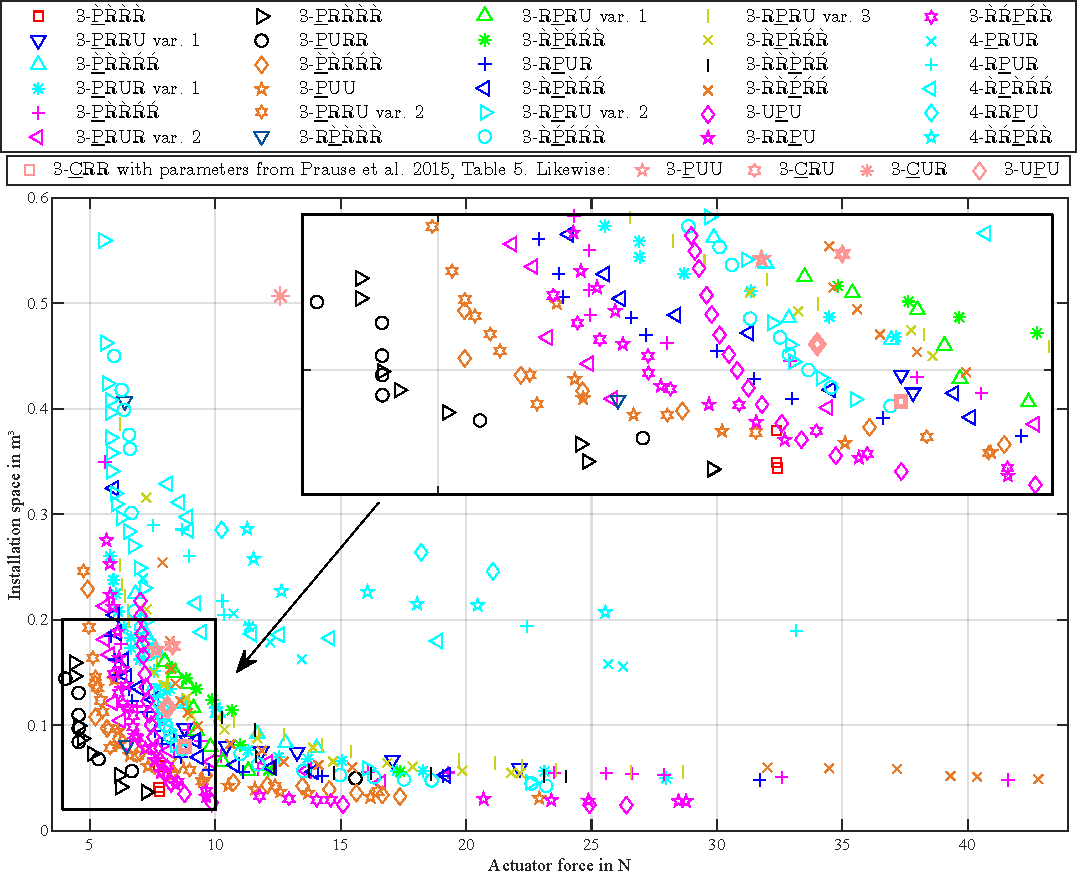
\includegraphics{Figures/handlingpkm_pareto_actforce_installspace_groups_onlypoints_prismatic.pdf}
  \end{adjustwidth}
  \caption[Handling task: \propername{Pareto} fronts for robots with prismatic actuation using only 27 reference points]{\propername{Pareto} fronts for robots with prismatic actuation using only 27 reference points.}%
\label{fig:handlingpkm_pareto_prismatic_onlypoints}
\end{figure}


\begin{figure}[H]
%
\begin{adjustwidth}{-\extralength}{0cm}
  \centering
  \graphicspath{{Figures}}
  \input{./Figures/handlingpkm_robots_reference.pdf_tex}
\end{adjustwidth}
%
\caption{\hl{Visualization} %
  %
  of the 3T0R parallel robots with parameters from \cite{PrauseChaCor2015}, listed in the bottom of Tables~\ref{tab:handlingpkm_results_pris}~and~\ref{tab:handlingpkm_results_pris_dh}.}
\label{fig:handlingpkm_robots_reference}
\end{figure}

\begin{figure}[H]
\vspace{0.1cm} %
\begin{adjustwidth}{-\extralength}{0cm}
  %
  \begin{overpic}
    {Figures/boxplots_handlingpkm/handlingpkm_boxplot_actforce_PrauseChaCor2015_collcheck1.pdf}
    \put(110,0){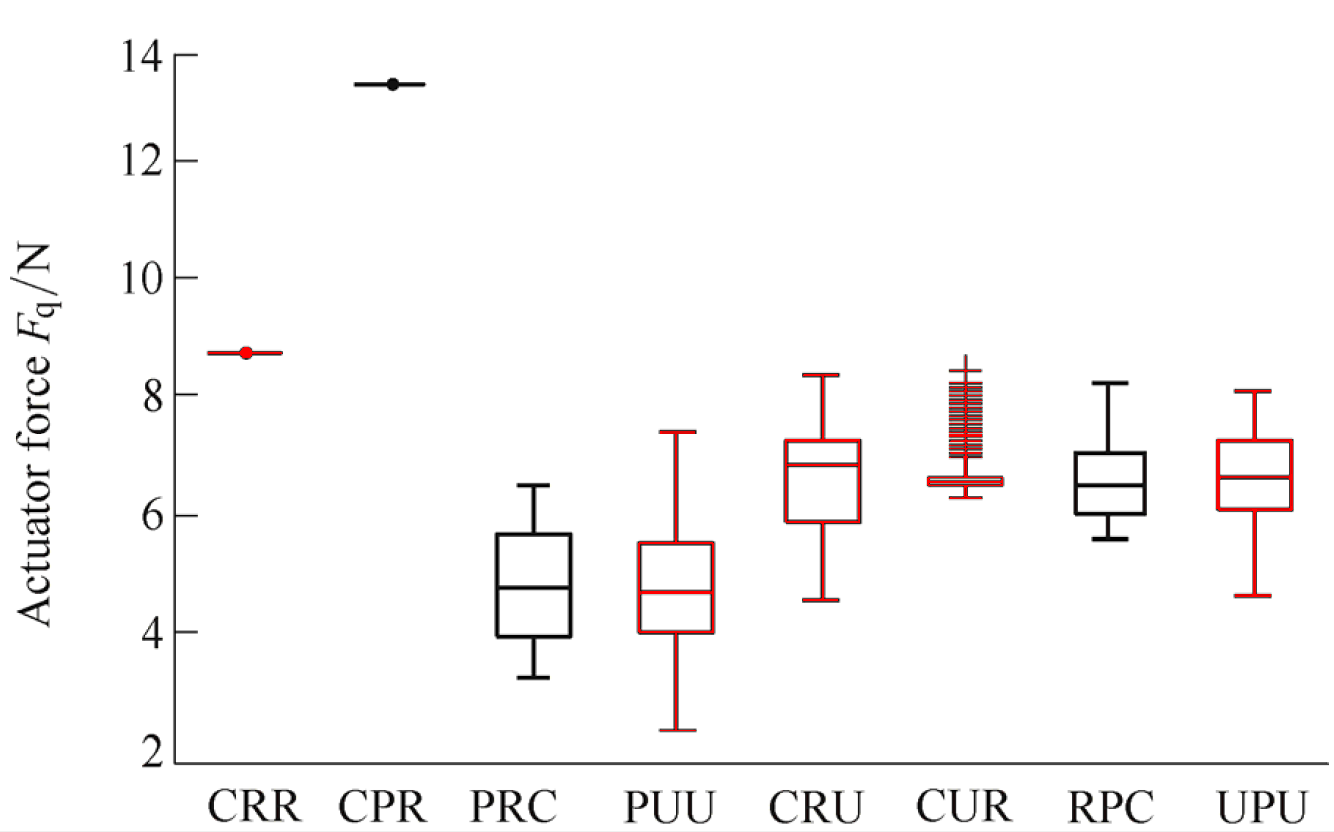
\includegraphics[width=8.2cm]{Figures/boxplots_handlingpkm/PrauseChaCor2015_Fig5.png}}
    \put(0,0){\textbf{(a)}}
    \put(110,0){\textbf{(b)}}
  \end{overpic} \\[0.5cm]
  \begin{overpic}
    {Figures/boxplots_handlingpkm/handlingpkm_boxplot_poserr_PrauseChaCor2015_collcheck1.pdf}
    \put(110,0){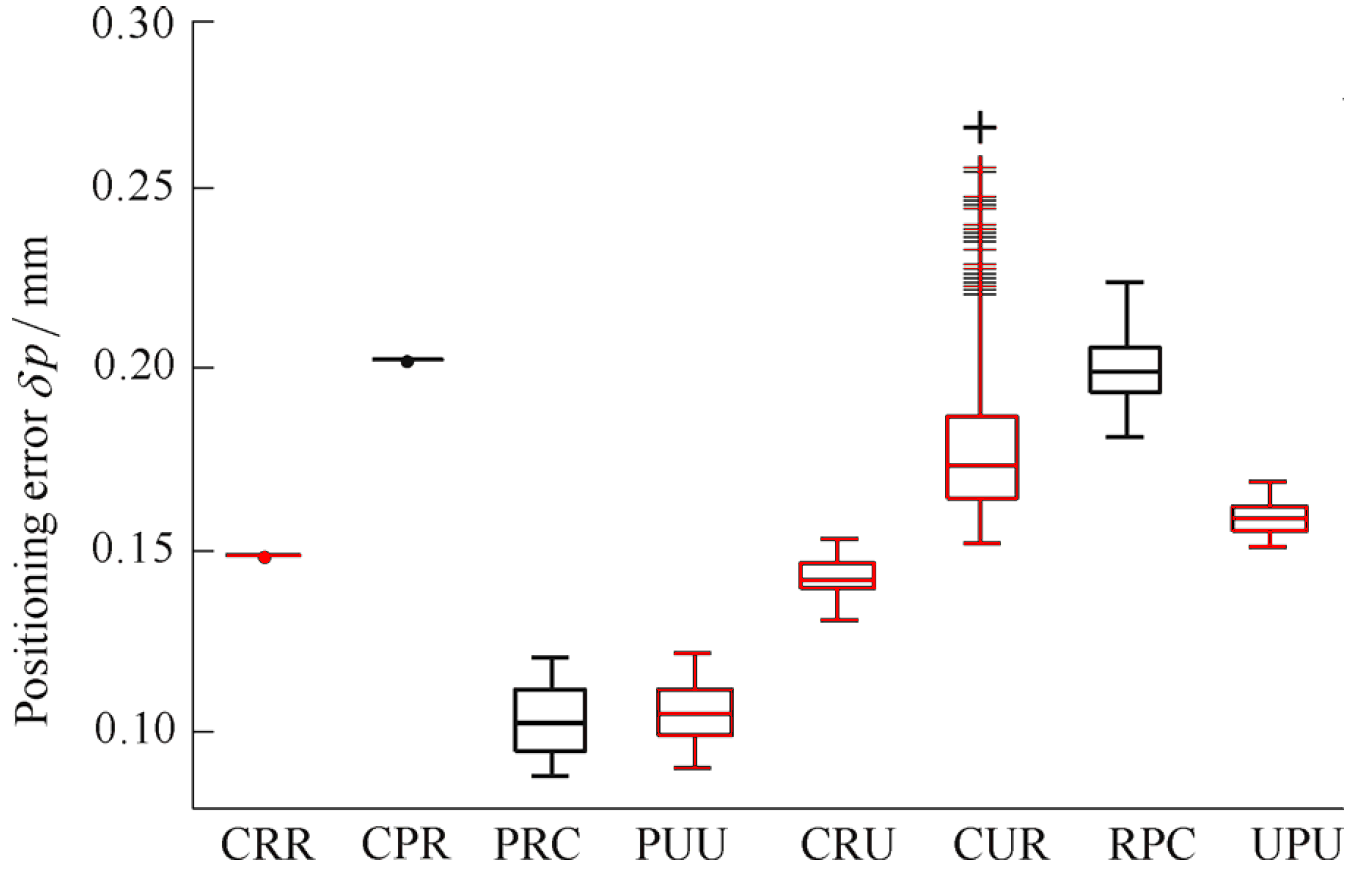
\includegraphics[height=4.9cm]{Figures/boxplots_handlingpkm/PrauseChaCor2015_Fig9.png}}
    \put(0,0){\textbf{(c)}}
    \put(110,0){\textbf{(d)}}
  \end{overpic} \\[0.5cm]
  \begin{overpic}
    {Figures/boxplots_handlingpkm/handlingpkm_boxplot_dexterity_PrauseChaCor2015_collcheck1.pdf}
    \put(110,0){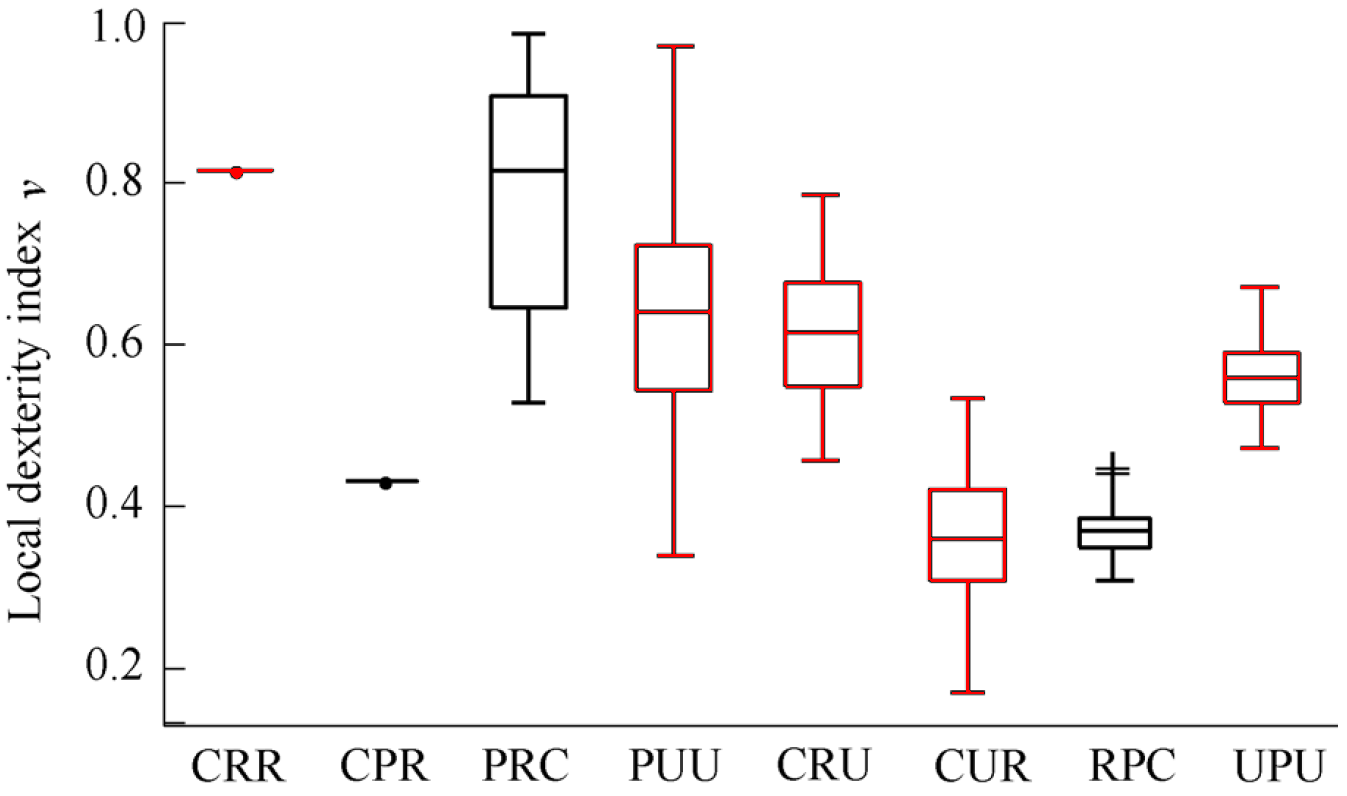
\includegraphics[height=4.9cm]{Figures/boxplots_handlingpkm/PrauseChaCor2015_Fig10.png}}
    \put(0,0){\textbf{(e)}}
    \put(110,0){\textbf{(f)}}
  \end{overpic} \\[0.15cm]
\end{adjustwidth}
%
\caption{Distribution of actuator force (\textbf{a},\textbf{b}), position error/precision (\textbf{c},\textbf{d}), and dexterity (\textbf{e},\textbf{f}) as performance criterion computed with parameters from Table~4 of \cite{PrauseChaCor2015} with this paper's implementation (left side) in comparison to the {original} results obtained from \cite{PrauseChaCor2015} (right side, with structures for comparison in red)}
\label{fig:handlingpkm_boxplot_PrauseChaCor2015}
%
\end{figure}

%

%
%
%
%
%
%
%
%
%

%


\begin{figure}[H]
\begin{adjustwidth}{-\extralength}{0cm}
  \centering
  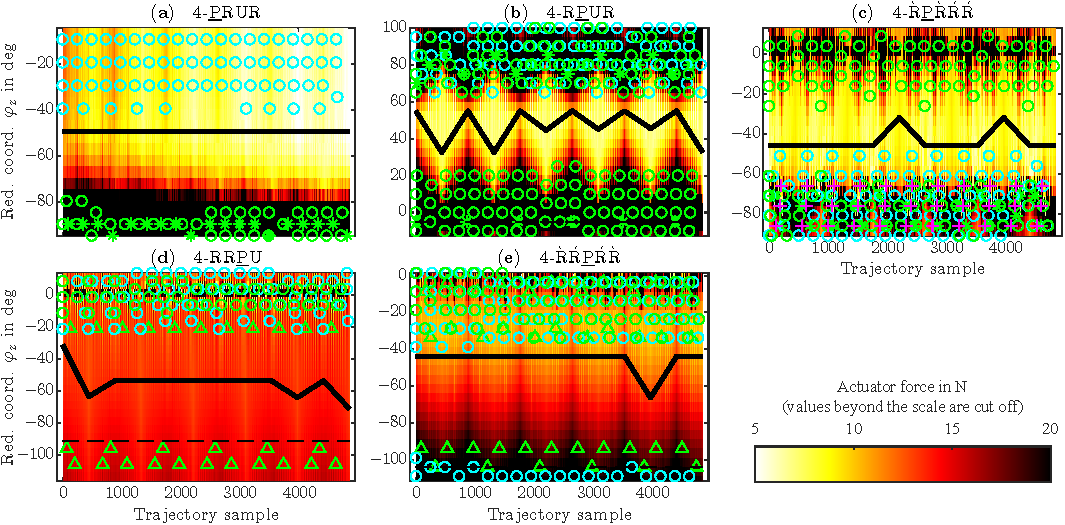
\includegraphics{Figures/handlingpkm_perfmaps_default_prismatic_multi_actforce_maxactforce.pdf}
\end{adjustwidth}
\caption{Performance
  maps for the prismatic-actuation parallel robots of Figure~\ref{fig:handlingpkm_robots_3T1R_pris} with maximum actuator force as IK objective and heat-map criterion. For marker legend, see below in Figure~\ref{fig:handlingpkm_perfmaps_multi_actforce_rev}.}
\label{fig:handlingpkm_perfmaps_multi_actforce_pris}
\end{figure}

\vspace{-12pt}
\begin{figure}[H]
\begin{adjustwidth}{-\extralength}{0cm}
  \centering
  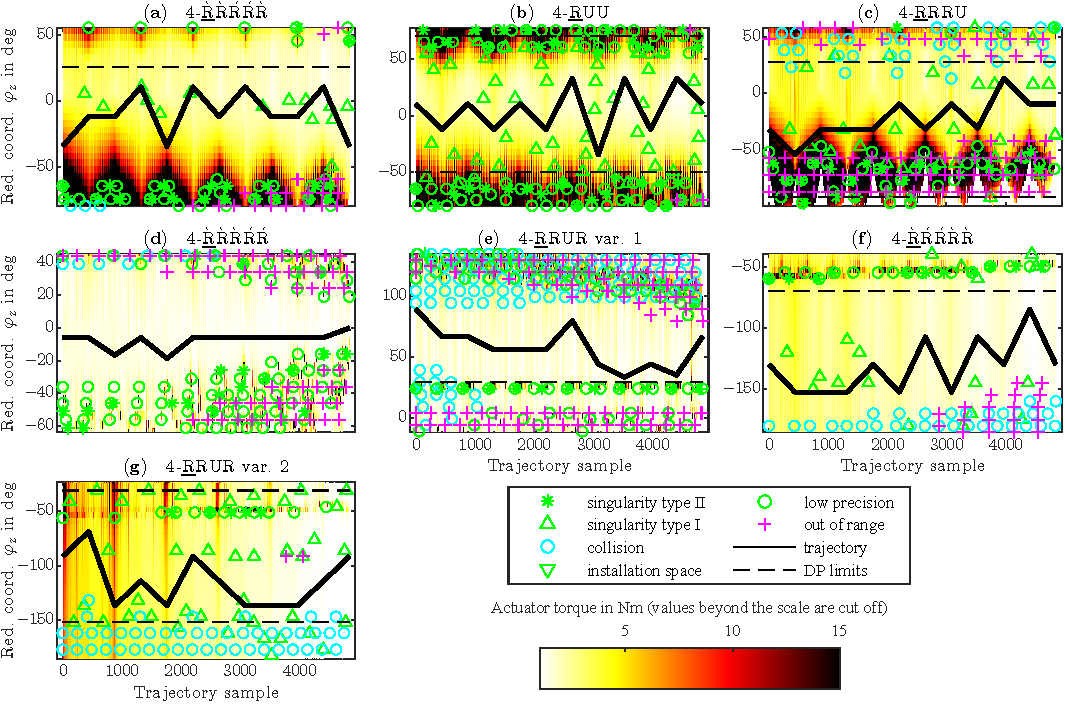
\includegraphics{Figures/handlingpkm_perfmaps_default_revolute_multi_actforce_maxactforce.pdf}
\end{adjustwidth}
\caption{Performance
  maps for the  revolute-actuation parallel robots of Figure~\ref{fig:handlingpkm_robots_3T1R_rev} with maximum actuator torque as IK objective and heat-map criterion.}
\label{fig:handlingpkm_perfmaps_multi_actforce_rev}
\end{figure}

\begin{figure}[H]
\begin{adjustwidth}{-\extralength}{0cm}
  \centering
  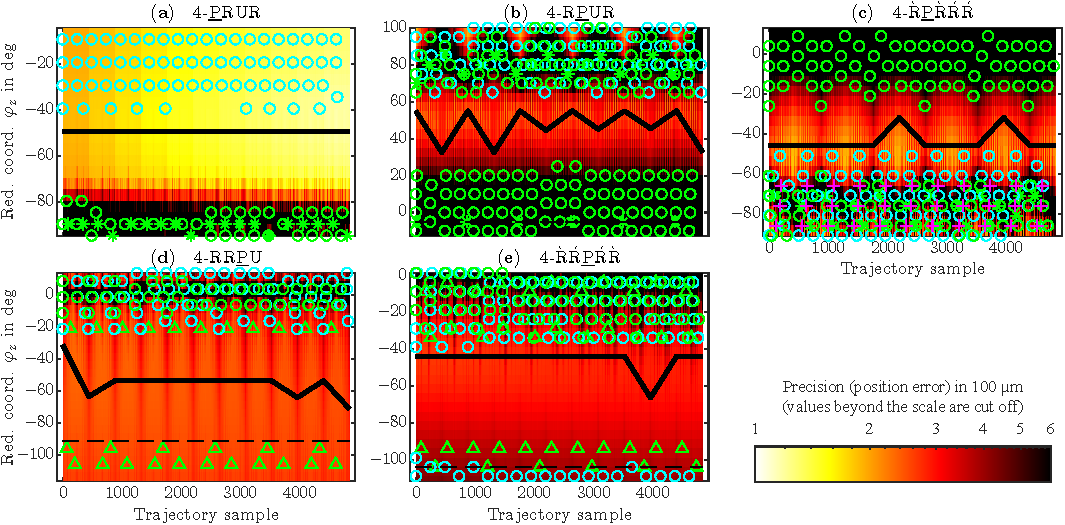
\includegraphics{Figures/handlingpkm_perfmaps_default_prismatic_multi_positionerror_maxactforce.pdf}
\end{adjustwidth}
\caption{Performance
  maps for the prismatic-actuation parallel robots of Figure~\ref{fig:handlingpkm_robots_3T1R_pris} with position error (precision) as heat-map criterion and trajectory from Figure~\ref{fig:handlingpkm_perfmaps_multi_actforce_pris}. For marker legend, see below in Figure~\ref{fig:handlingpkm_perfmaps_multi_poserr_rev}.}
\label{fig:handlingpkm_perfmaps_multi_poserr_pris}
\end{figure}

\vspace{-12pt}
\begin{figure}[H]
\begin{adjustwidth}{-\extralength}{0cm}
  \centering
  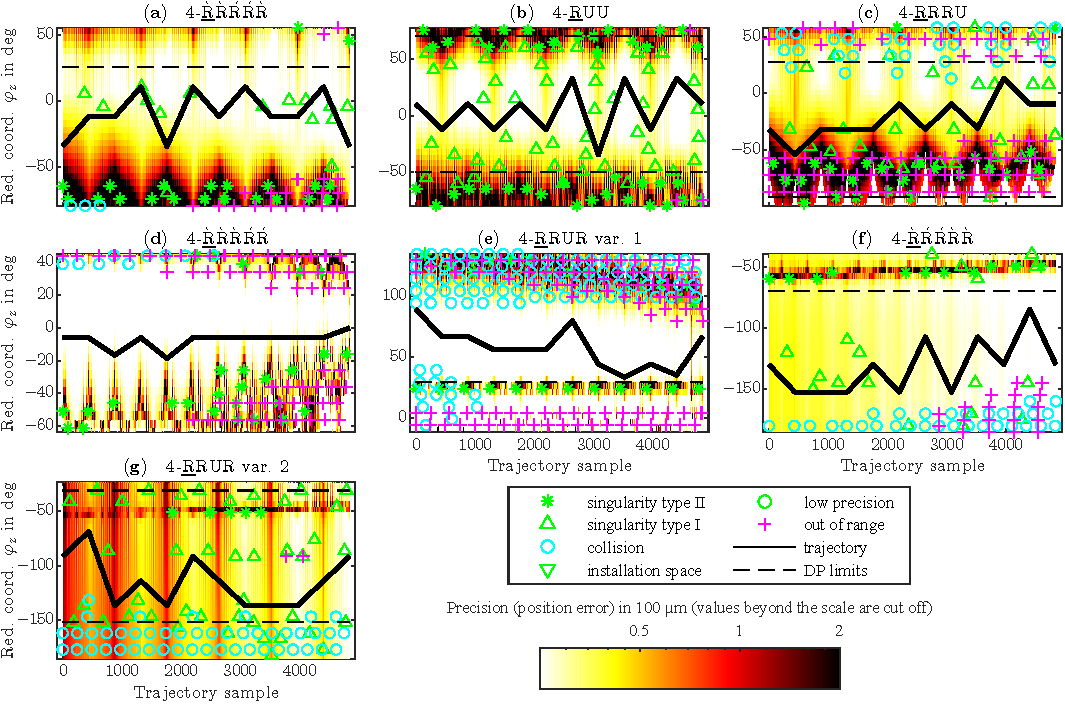
\includegraphics{Figures/handlingpkm_perfmaps_default_revolute_multi_positionerror_maxactforce.pdf}
\end{adjustwidth}
\caption{Performance
  maps for the revolute-actuation parallel robots of Figure~\ref{fig:handlingpkm_robots_3T1R_rev} with position error as heat-map criterion and trajectory from Figure~\ref{fig:handlingpkm_perfmaps_multi_actforce_rev}. Color scale is different than in Figure~\ref{fig:handlingpkm_perfmaps_multi_poserr_pris}~above.}
\label{fig:handlingpkm_perfmaps_multi_poserr_rev}
\end{figure} 

\begin{figure}[H]
\begin{adjustwidth}{-\extralength}{0cm}
  \centering
  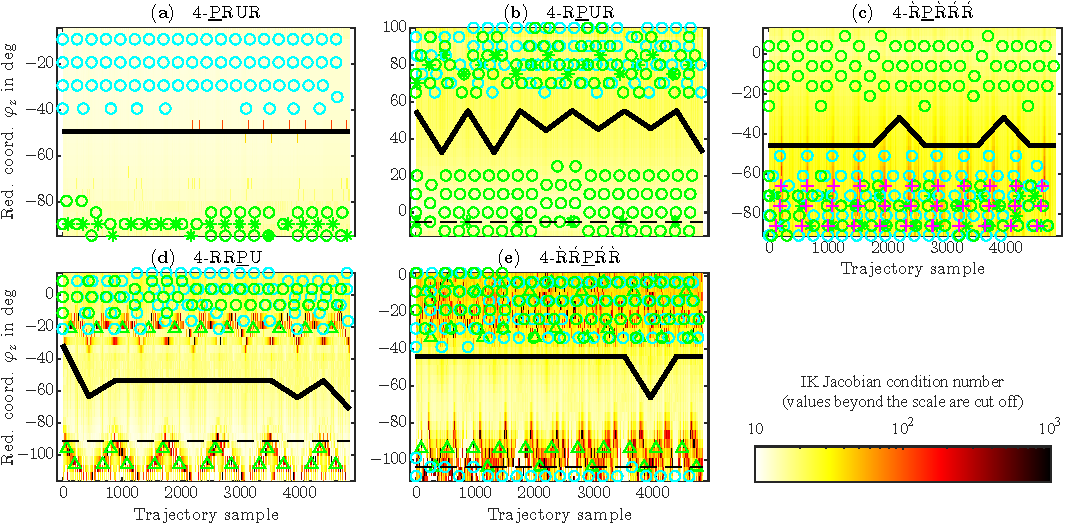
\includegraphics{Figures/handlingpkm_perfmaps_default_prismatic_multi_cond_ikjac_maxactforce.pdf}
\end{adjustwidth}
\caption{Performance
  maps for the prismatic-actuation parallel robots of Figure~\ref{fig:handlingpkm_robots_3T1R_pris} with IK-\propername{Jacobian} condition number as heat-map criterion and trajectory from Figure~\ref{fig:handlingpkm_perfmaps_multi_actforce_pris}. For marker legend, see below in Figure~\ref{fig:handlingpkm_perfmaps_multi_condikjac_rev}.}
\label{fig:handlingpkm_perfmaps_multi_condikjac_pris}
\end{figure} 

\vspace{-12pt}
\begin{figure}[H]
\begin{adjustwidth}{-\extralength}{0cm}
  \centering
  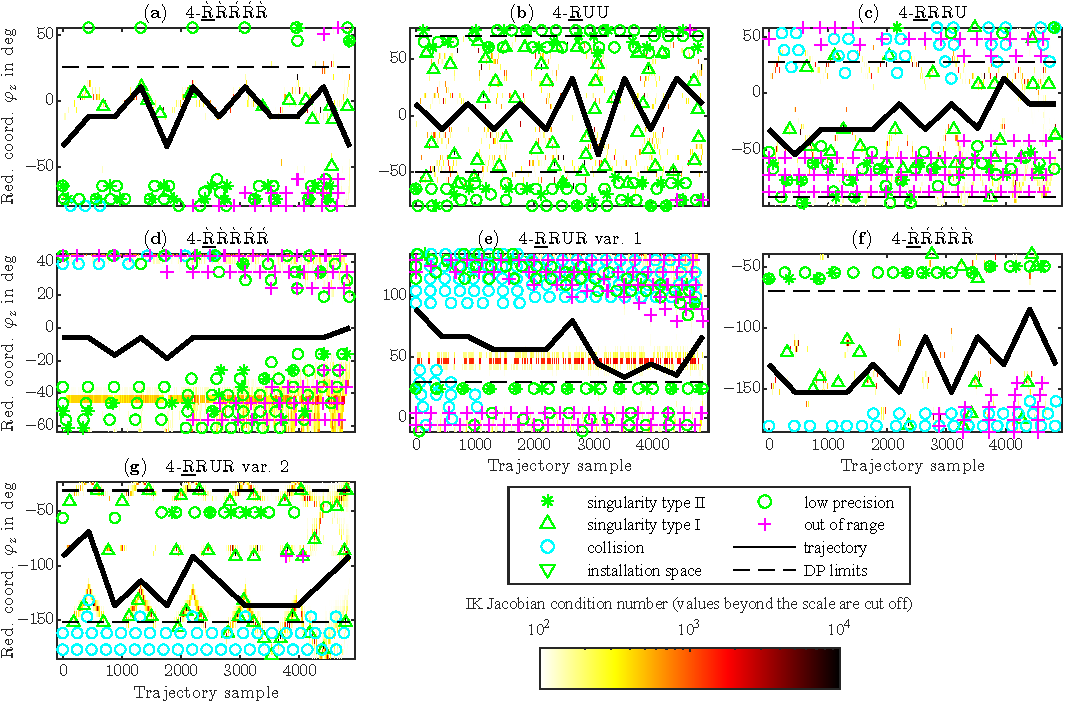
\includegraphics{Figures/handlingpkm_perfmaps_default_revolute_multi_cond_ikjac_maxactforce.pdf}
\end{adjustwidth}
\caption{Performance
  maps for the revolute-actuation parallel robots of Figure~\ref{fig:handlingpkm_robots_3T1R_rev} with IK-\propername{Jacobian} condition number as heat-map criterion and trajectory from Figure~\ref{fig:handlingpkm_perfmaps_multi_actforce_rev}. Color scale is different than in Figure~\ref{fig:handlingpkm_perfmaps_multi_condikjac_pris} above.}
\label{fig:handlingpkm_perfmaps_multi_condikjac_rev}
\end{figure} 


\clearpage %



\ifgrammarly
	\theendnotes %
	\newpage
\fi

%
%
\begin{adjustwidth}{-\extralength}{0cm}
%
%

\reftitle{References}

%
%

%
%
%
\externalbibliography{yes}
\bibliography{references_3460172}




%
%
%
%
%
%
%
%
%

%
%
%

%
%
%
%
%
%
%
%
\PublishersNote{}
%
\end{adjustwidth}
%
\end{document}
